\documentclass[11pt]{book}
 
\newcommand{\reporttitle}{Introduction to Multi-Dimensional Hawkes' Self-Exciting Point Processes: Simulation, Estimation, Adaptative Kernels and Changepoint Analysis.}
\newcommand{\reportauthor}{Niels D. C. CARIOU KOTLAREK}
\newcommand{\course}{Summer Project}
\newcommand{\professor}{Ed COHEN}
% include file with configuration.
\usepackage[utf8]{inputenc}
\usepackage[T1]{fontenc}

\usepackage[left=2.5cm,right=2.5cm,top=2cm,bottom=3cm]{geometry}%réglages des marges du document selon vos préférences ou celles de votre établissemant
\setlength{\headheight}{15pt}% hauteur de l'entête

\usepackage{array}  %pour les array et binomes de newton 
\usepackage{amsmath,amsfonts,amssymb}%extensions de l'ams pour les mathématiques
\usepackage{amsthm} %pour les théoremes
\usepackage{colortbl}
\usepackage[dvipsnames]{xcolor}
\usepackage{comment} % pour les commentaires
\usepackage{dsfont} %fonction indicatrice
\usepackage{fancybox} %pour shadow box
\usepackage[Rejne]{fncychap}%pour de jolis titres de chapitres voir la doc pour d'autres styles.
\usepackage{fancyhdr}%pour les entêtes et pieds de pages
\usepackage{graphicx}%pour insérer images et pdf entre autres
\graphicspath{{images/}}%pour spécifier le chemin d'accès aux images
\usepackage{lmodern}	%celui ci et le suivant pour les boites
\usepackage{shorttoc}%pour la réalisation d'un sommaire.
\usepackage[most]{tcolorbox}

\usepackage{lipsum} %to test paragraphs
\usepackage{verbatim} %for writing as code
\usepackage{fancyvrb} %this is for reducing size of verbatim
\usepackage{subfig} %for having the figures next to each other
\usepackage{stmaryrd} % pacakge for double brackets, notation for integers.
\usepackage{url} % for path in names or url in general.

\usepackage[ruled,vlined]{algorithm2e} % for algorithms
\usepackage{lscape} % for the biiiig table at the end of the document
\usepackage{rotating} % for the biiiig table at the end of the document



\hbadness = 15000 % prevention against warning
\hfuzz = 100 pt % do not trigger any warning related to hbox. I.E. that the line is too long. I had plenty of such useless warnings. 
\vbadness=\maxdimen % against warning




%%%%%=======================================================================tikz
\usepackage{tikz}
\usetikzlibrary{arrows.meta}
\usepackage{mathdots}
\usepackage{mathtools}
\usepackage{pdflscape}
\usepackage{pgfplots}
\usepackage{siunitx}
\usepackage{slashed}
\usepackage{tabularx}
\usepackage{tikz}
\usepackage{tkz-euclide}
\usepackage[normalem]{ulem}
\usepackage[all]{xy}
\usepackage{imakeidx}



\pgfarrowsdeclarecombine{twolatex'}{twolatex'}{latex'}{latex'}{latex'}{latex'}
\tikzset{->>/.style = {decoration={markings,
                                  mark=at position 1 with {\arrow[scale=2]{latex'}}},
                      postaction={decorate}}}
\tikzset{<-/.style = {decoration={markings,
                                  mark=at position 0 with {\arrowreversed[scale=2]{latex'}}},
                      postaction={decorate}}}
\tikzset{<->/.style = {decoration={markings,
                                   mark=at position 0 with {\arrowreversed[scale=2]{latex'}},
                                   mark=at position 1 with {\arrow[scale=2]{latex'}}},
                       postaction={decorate}}}
\tikzset{->-/.style = {decoration={markings,
                                   mark=at position #1 with {\arrow[scale=2]{latex'}}},
                       postaction={decorate}}}
\tikzset{-<-/.style = {decoration={markings,
                                   mark=at position #1 with {\arrowreversed[scale=2]{latex'}}},
                       postaction={decorate}}}
\tikzset{<<-/.style = {decoration={markings,
                                  mark=at position 0 with {\arrowreversed[scale=2]{twolatex'}}},
                      postaction={decorate}}}
\tikzset{<<->>/.style = {decoration={markings,
                                   mark=at position 0 with {\arrowreversed[scale=2]{twolatex'}},
                                   mark=at position 1 with {\arrow[scale=2]{twolatex'}}},
                       postaction={decorate}}}
\tikzset{->>-/.style = {decoration={markings,
                                   mark=at position #1 with {\arrow[scale=2]{twolatex'}}},
                       postaction={decorate}}}
\tikzset{-<<-/.style = {decoration={markings,
                                   mark=at position #1 with {\arrowreversed[scale=2]{twolatex'}}},
                       postaction={decorate}}}

\tikzset{circ/.style = {fill, circle, inner sep = 0, minimum size = 3}}
\tikzset{scirc/.style = {fill, circle, inner sep = 0, minimum size = 1.5}}
\tikzset{mstate/.style={circle, draw, blue, text=black, minimum width=0.7cm}}

\tikzset{eqpic/.style={baseline={([yshift=-.5ex]current bounding box.center)}}}
\tikzset{commutative diagrams/.cd,cdmap/.style={/tikz/column 1/.append style={anchor=base east},/tikz/column 2/.append style={anchor=base west},row sep=tiny}}

\definecolor{mblue}{rgb}{0.17, 0.27, 0.9}
\definecolor{morange}{rgb}{1, 0.48, 0}
\definecolor{mgreen}{rgb}{0, 0.4, 0.1}
\definecolor{mred}{rgb}{0.8, 0.09, 0.09}



%%%%%=========================================================================tikz







%%% définition de couleurs pour théoremes
\definecolor{vert}{RGB}{0,181,0}
\definecolor{oran}{RGB}{223,74,0}
\definecolor{viol}{RGB}{134,0,175}
\definecolor{mauv}{RGB}{200,0,115}
\definecolor{roug}{RGB}{215,15,0}	

%%%% couleurs listes :
\definecolor{abricot}{rgb}{0.901,0.494,0.188}
\definecolor{absinthe}{rgb}{0.498,0.866,0.298}
\definecolor{acajou}{rgb}{0.533,0.258,0.113}
\definecolor{aiguemarine}{rgb}{0.474,0.972,0.972}
\definecolor{ailedecorbeau}{rgb}{0.0,0.0,0.0}
\definecolor{albatre}{rgb}{0.996,0.996,0.996}
\definecolor{alezan}{rgb}{0.654,0.403,0.149}
\definecolor{amande}{rgb}{0.509,0.768,0.423}
\definecolor{amarante}{rgb}{0.568,0.156,0.231}
\definecolor{ambrejaune}{rgb}{0.941,0.764,0.0}
\definecolor{ambrerouge}{rgb}{0.678,0.223,0.054}
\definecolor{amethyste}{rgb}{0.533,0.301,0.654}
\definecolor{anthracite}{rgb}{0.188,0.188,0.188}
\definecolor{aquilain}{rgb}{0.678,0.309,0.035}
\definecolor{ardoise}{rgb}{0.352,0.368,0.419}
\definecolor{argent}{rgb}{0.807,0.807,0.807}
\definecolor{argile}{rgb}{0.937,0.937,0.937}
\definecolor{asperge}{rgb}{0.482,0.627,0.356}
\definecolor{aubergine}{rgb}{0.215,0.0,0.156}
\definecolor{auburn}{rgb}{0.615,0.243,0.047}
\definecolor{aurore}{rgb}{1.0,0.796,0.376}
\definecolor{avocat}{rgb}{0.337,0.509,0.011}
\definecolor{azur}{rgb}{0.0,0.498,1.0}
\definecolor{azurbrume}{rgb}{0.941,1.0,1.0}
\definecolor{azurclair}{rgb}{0.454,0.815,0.945}
\definecolor{azurin}{rgb}{0.662,0.917,0.996}
\definecolor{baillet}{rgb}{0.682,0.392,0.176}
\definecolor{banane}{rgb}{0.819,0.713,0.023}
\definecolor{basane}{rgb}{0.545,0.423,0.258}
\definecolor{beige}{rgb}{0.784,0.678,0.498}
\definecolor{beigeclair}{rgb}{0.96,0.96,0.862}
\definecolor{beigeasse}{rgb}{0.686,0.654,0.482}
\definecolor{beurre}{rgb}{0.941,0.89,0.419}
\definecolor{beurrefrais}{rgb}{1.0,0.956,0.552}
\definecolor{bis}{rgb}{0.462,0.435,0.392}
\definecolor{bisque}{rgb}{1.0,0.894,0.768}
\definecolor{bistre}{rgb}{0.521,0.427,0.301}
\definecolor{bitume}{rgb}{0.305,0.239,0.156}
\definecolor{blanc}{rgb}{1.0,1.0,1.0}
\definecolor{blanccasse}{rgb}{0.996,0.996,0.886}
\definecolor{blanccreme}{rgb}{0.992,0.945,0.721}
\definecolor{blancdargent}{rgb}{0.996,0.996,0.996}
\definecolor{blancdespagne}{rgb}{0.996,0.992,0.941}
\definecolor{blancdelait}{rgb}{0.984,0.988,0.98}
\definecolor{blancdemeudon}{rgb}{0.996,0.992,0.941}
\definecolor{blancdezinc}{rgb}{0.964,0.996,0.996}
\definecolor{blanclunaire}{rgb}{0.956,0.996,0.996}
\definecolor{ble}{rgb}{0.909,0.839,0.188}
\definecolor{blet}{rgb}{0.356,0.235,0.066}
\definecolor{bleu}{rgb}{0.105,0.003,0.607}
\definecolor{bleuacier}{rgb}{0.227,0.556,0.729}
\definecolor{bleuardoise}{rgb}{0.407,0.435,0.549}
\definecolor{bleubarbeau}{rgb}{0.329,0.447,0.682}
\definecolor{bleucanard}{rgb}{0.015,0.545,0.603}
\definecolor{bleuceleste}{rgb}{0.149,0.768,0.925}
\definecolor{bleuceruleen}{rgb}{0.207,0.478,0.717}
\definecolor{bleucharrette}{rgb}{0.556,0.635,0.776}
\definecolor{bleuciel}{rgb}{0.466,0.709,0.996}
\definecolor{bleudeberlin}{rgb}{0.141,0.266,0.36}
\definecolor{bleudecobalt}{rgb}{0.133,0.258,0.486}
\definecolor{bleudefrance}{rgb}{0.192,0.549,0.905}
\definecolor{bleudeminuit}{rgb}{0.0,0.2,0.4}
\definecolor{bleudeprusse}{rgb}{0.141,0.266,0.36}
\definecolor{bleudesmersdusud}{rgb}{0.0,0.8,0.796}
\definecolor{bleudragee}{rgb}{0.874,0.949,1.0}
\definecolor{bleuelectrique}{rgb}{0.172,0.458,1.0}
\definecolor{bleufumee}{rgb}{0.733,0.823,0.882}
\definecolor{bleugivre}{rgb}{0.501,0.815,0.815}
\definecolor{bleuguede}{rgb}{0.337,0.45,0.603}
\definecolor{bleuhussard}{rgb}{0.141,0.266,0.36}
\definecolor{bleuklein}{rgb}{0.0,0.184,0.654}
\definecolor{bleulavande}{rgb}{0.588,0.513,0.925}
\definecolor{bleumajorelle}{rgb}{0.376,0.313,0.862}
\definecolor{bleumarine}{rgb}{0.011,0.133,0.298}
\definecolor{bleunuit}{rgb}{0.058,0.019,0.419}
\definecolor{bleuoutremer}{rgb}{0.106,0.004,0.608}
\definecolor{bleupaon}{rgb}{0.023,0.466,0.564}
\definecolor{bleupersan}{rgb}{0.4,0.0,1.0}
\definecolor{bleupetrole}{rgb}{0.113,0.282,0.317}
\definecolor{bleuprimaire}{rgb}{0.0,0.0,1.0}
\definecolor{bleuroi}{rgb}{0.192,0.549,0.905}
\definecolor{bleusaphir}{rgb}{0.003,0.192,0.705}
\definecolor{bleuturquin}{rgb}{0.258,0.356,0.541}
\definecolor{bleuturquoise}{rgb}{0.145,0.992,0.913}
\definecolor{blond}{rgb}{0.886,0.737,0.454}
\definecolor{blondvenitien}{rgb}{0.905,0.658,0.329}
\definecolor{bordeaux}{rgb}{0.427,0.027,0.101}
\definecolor{bourgogne}{rgb}{0.419,0.05,0.05}
\definecolor{boutondor}{rgb}{0.988,0.862,0.07}
\definecolor{brique}{rgb}{0.517,0.18,0.105}
\definecolor{bronze}{rgb}{0.38,0.305,0.101}
\definecolor{broudenoix}{rgb}{0.247,0.133,0.015}
\definecolor{brun}{rgb}{0.356,0.235,0.066}
\definecolor{brunclair}{rgb}{0.803,0.521,0.247}
\definecolor{bureau}{rgb}{0.419,0.341,0.192}
\definecolor{byzantin}{rgb}{0.741,0.2,0.643}
\definecolor{byzantium}{rgb}{0.439,0.16,0.388}
\definecolor{cacadoie}{rgb}{0.803,0.803,0.05}
\definecolor{cacao}{rgb}{0.38,0.294,0.227}
\definecolor{cachou}{rgb}{0.184,0.105,0.047}
\definecolor{cafe}{rgb}{0.274,0.18,0.003}
\definecolor{cafeaulait}{rgb}{0.47,0.368,0.184}
\definecolor{cannelle}{rgb}{0.494,0.345,0.207}
\definecolor{capucine}{rgb}{1.0,0.368,0.301}
\definecolor{caramel}{rgb}{0.494,0.2,0.0}
\definecolor{carmin}{rgb}{0.588,0.0,0.094}
\definecolor{carotte}{rgb}{0.956,0.4,0.105}
\definecolor{cassis}{rgb}{0.227,0.007,0.05}
\definecolor{celadon}{rgb}{0.513,0.65,0.592}
\definecolor{cerise}{rgb}{0.87,0.192,0.388}
\definecolor{ceruse}{rgb}{0.996,0.996,0.996}
\definecolor{chair}{rgb}{0.996,0.764,0.674}
\definecolor{chamois}{rgb}{0.815,0.752,0.478}
\definecolor{champagne}{rgb}{0.984,0.949,0.717}
\definecolor{charbonneux}{rgb}{0.0,0.0,0.062}
\definecolor{chartreuse}{rgb}{0.498,1.0,0.0}
\definecolor{chataigne}{rgb}{0.501,0.427,0.352}
\definecolor{chatain}{rgb}{0.545,0.423,0.258}
\definecolor{chaudron}{rgb}{0.521,0.325,0.058}
\definecolor{chenu}{rgb}{0.996,0.996,0.996}
\definecolor{chocolat}{rgb}{0.352,0.227,0.133}
\definecolor{cinabre}{rgb}{0.858,0.09,0.007}
\definecolor{citron}{rgb}{0.968,1.0,0.235}
\definecolor{citrouille}{rgb}{0.874,0.427,0.078}
\definecolor{clarissimo}{rgb}{0.725,0.698,0.462}
\definecolor{claro}{rgb}{0.517,0.352,0.231}
\definecolor{claroclaro}{rgb}{0.729,0.607,0.38}
\definecolor{colombin}{rgb}{0.415,0.27,0.364}
\definecolor{colorado}{rgb}{0.439,0.207,0.086}
\definecolor{coloradoclaro}{rgb}{0.415,0.294,0.129}
\definecolor{coquelicot}{rgb}{0.776,0.031,0.0}
\definecolor{coquilledoeuf}{rgb}{0.992,0.913,0.878}
\definecolor{corail}{rgb}{0.905,0.243,0.003}
\definecolor{cramoisi}{rgb}{0.862,0.078,0.235}
\definecolor{creme}{rgb}{0.992,0.945,0.721}
\definecolor{cuissedenymphe}{rgb}{0.996,0.905,0.941}
\definecolor{cuissedenympheemue}{rgb}{1.0,0.411,0.705}
\definecolor{cuivre}{rgb}{0.701,0.403,0.0}
\definecolor{cyan}{rgb}{0.168,0.98,0.98}
\definecolor{cyansecondaire}{rgb}{0.0,1.0,1.0}
\definecolor{ceruleum}{rgb}{0.207,0.478,0.717}
\definecolor{denim}{rgb}{0.082,0.376,0.741}
\definecolor{dium}{rgb}{0.043,0.086,0.086}
\definecolor{ebene}{rgb}{0.0,0.0,0.0}
\definecolor{ecarlate}{rgb}{0.929,0.0,0.0}
\definecolor{ecru}{rgb}{0.996,0.996,0.878}
\definecolor{emeraude}{rgb}{0.003,0.843,0.345}
\definecolor{etainoxyde}{rgb}{0.729,0.729,0.729}
\definecolor{etainpur}{rgb}{0.929,0.929,0.929}
\definecolor{fauve}{rgb}{0.678,0.309,0.035}
\definecolor{fer}{rgb}{0.517,0.517,0.517}
\definecolor{feuvif}{rgb}{1.0,0.286,0.003}
\definecolor{feuillemorte}{rgb}{0.6,0.317,0.168}
\definecolor{flave}{rgb}{0.901,0.901,0.592}
\definecolor{fleurdesoufre}{rgb}{1.0,1.0,0.419}
\definecolor{fraise}{rgb}{0.749,0.188,0.188}
\definecolor{fraiseecrasee}{rgb}{0.643,0.141,0.141}
\definecolor{framboise}{rgb}{0.78,0.172,0.282}
\definecolor{fuchsia}{rgb}{0.956,0.0,0.631}
\definecolor{garance}{rgb}{0.933,0.062,0.062}
\definecolor{glauque}{rgb}{0.392,0.607,0.533}
\definecolor{glycine}{rgb}{0.788,0.627,0.862}
\definecolor{grege}{rgb}{0.733,0.682,0.596}
\definecolor{grenadine}{rgb}{0.913,0.219,0.247}
\definecolor{grenat}{rgb}{0.431,0.043,0.078}
\definecolor{gris}{rgb}{0.376,0.376,0.376}
\definecolor{grisacier}{rgb}{0.686,0.686,0.686}
\definecolor{grisanthracite}{rgb}{0.188,0.188,0.188}
\definecolor{grisdelin}{rgb}{0.823,0.792,0.925}
\definecolor{grisdemaure}{rgb}{0.407,0.368,0.262}
\definecolor{grisdepayne}{rgb}{0.403,0.443,0.474}
\definecolor{grisfer}{rgb}{0.498,0.498,0.498}
\definecolor{grisfumee}{rgb}{0.733,0.823,0.882}
\definecolor{grisperle}{rgb}{0.807,0.807,0.807}
\definecolor{grisplomb}{rgb}{0.474,0.501,0.505}
\definecolor{grissouris}{rgb}{0.619,0.619,0.619}
\definecolor{gristaupe}{rgb}{0.274,0.247,0.196}
\definecolor{gristourdille}{rgb}{0.756,0.749,0.694}
\definecolor{gristourterelle}{rgb}{0.733,0.674,0.674}
\definecolor{groseille}{rgb}{0.811,0.039,0.113}
\definecolor{havane}{rgb}{0.58,0.498,0.376}
\definecolor{heliotrope}{rgb}{0.874,0.45,1.0}
\definecolor{hoto}{rgb}{0.0,0.0,0.0}
\definecolor{incarnadin}{rgb}{0.996,0.588,0.627}
\definecolor{incarnat}{rgb}{1.0,0.435,0.49}
\definecolor{indigo}{rgb}{0.18,0.0,0.423}
\definecolor{indigochaud}{rgb}{0.474,0.109,0.972}
\definecolor{indigoduweb}{rgb}{0.294,0.0,0.509}
\definecolor{indigoelectrique}{rgb}{0.435,0.0,1.0}
\definecolor{isabelle}{rgb}{0.47,0.368,0.184}
\definecolor{ivoire}{rgb}{1.0,1.0,0.831}
\definecolor{jade}{rgb}{0.529,0.913,0.564}
\definecolor{jais}{rgb}{0.0,0.0,0.0}
\definecolor{jauneaureolin}{rgb}{0.992,0.933,0.0}
\definecolor{jaunebanane}{rgb}{0.819,0.713,0.023}
\definecolor{jauneboutondor}{rgb}{0.964,0.862,0.07}
\definecolor{jaunecanari}{rgb}{0.905,0.941,0.05}
\definecolor{jaunechartreuse}{rgb}{0.874,1.0,0.0}
\definecolor{jaunecitron}{rgb}{0.968,1.0,0.235}
\definecolor{jaunedor}{rgb}{0.937,0.847,0.027}
\definecolor{jaunedechrome}{rgb}{0.929,1.0,0.047}
\definecolor{jaunedemars}{rgb}{0.933,0.819,0.325}
\definecolor{jaunedenaples}{rgb}{1.0,0.941,0.737}
\definecolor{jaunefleurdesoufre}{rgb}{1.0,1.0,0.419}
\definecolor{jauneimperial}{rgb}{1.0,0.894,0.211}
\definecolor{jaunemais}{rgb}{1.0,0.87,0.458}
\definecolor{jaunemimosa}{rgb}{0.996,0.972,0.423}
\definecolor{jaunemoutarde}{rgb}{0.78,0.811,0.0}
\definecolor{jaunenankin}{rgb}{0.968,0.886,0.411}
\definecolor{jaunepaille}{rgb}{0.996,0.89,0.278}
\definecolor{jaunepoussin}{rgb}{0.968,0.89,0.372}
\definecolor{jauneprimaire}{rgb}{1.0,1.0,0.0}
\definecolor{jaunesoufre}{rgb}{1.0,1.0,0.419}
\definecolor{kaki}{rgb}{0.58,0.505,0.168}
\definecolor{lapislazuli}{rgb}{0.149,0.38,0.611}
\definecolor{lavalliere}{rgb}{0.56,0.349,0.133}
\definecolor{lavande}{rgb}{0.588,0.513,0.925}
\definecolor{liedevin}{rgb}{0.674,0.117,0.266}
\definecolor{lilas}{rgb}{0.713,0.4,0.823}
\definecolor{lin}{rgb}{0.98,0.941,0.901}
\definecolor{maduro}{rgb}{0.215,0.184,0.145}
\definecolor{madurocolorado}{rgb}{0.356,0.235,0.066}
\definecolor{magentafonce}{rgb}{0.501,0.0,0.501}
\definecolor{magentafushia}{rgb}{0.858,0.0,0.45}
\definecolor{magentasecondaire}{rgb}{1.0,0.0,1.0}
\definecolor{mais}{rgb}{1.0,0.87,0.458}
\definecolor{malachite}{rgb}{0.121,0.627,0.333}
\definecolor{mandarine}{rgb}{0.996,0.639,0.278}
\definecolor{marine}{rgb}{0.011,0.133,0.298}
\definecolor{marron}{rgb}{0.345,0.16,0.0}
\definecolor{mastic}{rgb}{0.701,0.694,0.568}
\definecolor{mauve}{rgb}{0.831,0.45,0.831}
\definecolor{melon}{rgb}{0.87,0.596,0.086}
\definecolor{menthe}{rgb}{0.086,0.721,0.305}
\definecolor{menthealeau}{rgb}{0.329,0.976,0.552}
\definecolor{miel}{rgb}{0.854,0.701,0.039}
\definecolor{mordore}{rgb}{0.529,0.349,0.101}
\definecolor{moreau}{rgb}{0.0,0.0,0.0}
\definecolor{moutarde}{rgb}{0.78,0.811,0.0}
\definecolor{nacarat}{rgb}{0.988,0.364,0.364}
\definecolor{nankin}{rgb}{0.968,0.886,0.411}
\definecolor{neige}{rgb}{0.996,0.996,0.996}
\definecolor{noir}{rgb}{0.0,0.0,0.0}
\definecolor{noiranimal}{rgb}{0.0,0.0,0.0}
\definecolor{noircharbon}{rgb}{0.0,0.0,0.062}
\definecolor{noirdaniline}{rgb}{0.07,0.05,0.086}
\definecolor{noirdencre}{rgb}{0.0,0.0,0.0}
\definecolor{noirdivoire}{rgb}{0.0,0.0,0.0}
\definecolor{noirdecarbone}{rgb}{0.074,0.054,0.039}
\definecolor{noirdefumee}{rgb}{0.074,0.054,0.039}
\definecolor{noirdejais}{rgb}{0.0,0.0,0.0}
\definecolor{noiraud}{rgb}{0.184,0.117,0.054}
\definecolor{noisette}{rgb}{0.584,0.337,0.156}
\definecolor{ocrejaune}{rgb}{0.874,0.686,0.172}
\definecolor{ocrerouge}{rgb}{0.866,0.596,0.36}
\definecolor{olive}{rgb}{0.439,0.552,0.137}
\definecolor{opalin}{rgb}{0.949,1.0,1.0}
\definecolor{or}{rgb}{1.0,0.843,0.0}
\definecolor{orange}{rgb}{0.929,0.498,0.062}
\definecolor{orangebrulee}{rgb}{0.8,0.333,0.0}
\definecolor{orchidee}{rgb}{0.854,0.439,0.839}
\definecolor{orpiment}{rgb}{0.988,0.823,0.109}
\definecolor{orpindeperse}{rgb}{0.988,0.823,0.109}
\definecolor{oscuro}{rgb}{0.16,0.129,0.027}
\definecolor{paille}{rgb}{0.996,0.89,0.278}
\definecolor{papaye}{rgb}{1.0,0.937,0.835}
\definecolor{papierbulle}{rgb}{0.929,0.827,0.549}
\definecolor{parme}{rgb}{0.811,0.627,0.913}
\definecolor{passevelours}{rgb}{0.568,0.156,0.231}
\definecolor{pastel}{rgb}{0.337,0.45,0.603}
\definecolor{peche}{rgb}{0.992,0.749,0.717}
\definecolor{peluredoignon}{rgb}{0.835,0.517,0.564}
\definecolor{pervenche}{rgb}{0.8,0.8,1.0}
\definecolor{pinchard}{rgb}{0.8,0.8,0.8}
\definecolor{pistache}{rgb}{0.745,0.96,0.454}
\definecolor{platine}{rgb}{0.98,0.941,0.772}
\definecolor{plomb}{rgb}{0.474,0.501,0.505}
\definecolor{poildechameau}{rgb}{0.713,0.47,0.137}
\definecolor{ponceau}{rgb}{0.776,0.031,0.0}
\definecolor{prasin}{rgb}{0.298,0.65,0.419}
\definecolor{prune}{rgb}{0.505,0.078,0.325}
\definecolor{puce}{rgb}{0.305,0.086,0.035}
\definecolor{queuederenard}{rgb}{0.568,0.156,0.231}
\definecolor{queuedevacheclair}{rgb}{0.764,0.705,0.439}
\definecolor{queuedevachefonce}{rgb}{0.658,0.596,0.454}
\definecolor{reglisse}{rgb}{0.176,0.141,0.117}
\definecolor{rose}{rgb}{0.992,0.423,0.619}
\definecolor{rosebalais}{rgb}{0.768,0.411,0.56}
\definecolor{rosebonbon}{rgb}{0.976,0.258,0.619}
\definecolor{rosedragee}{rgb}{0.996,0.749,0.823}
\definecolor{rosefuchsia}{rgb}{0.992,0.247,0.572}
\definecolor{rosemountbatten}{rgb}{0.6,0.478,0.552}
\definecolor{rosethe}{rgb}{1.0,0.525,0.415}
\definecolor{rosevif}{rgb}{1.0,0.0,0.498}
\definecolor{rouge}{rgb}{1.0,0.0,0.0}
\definecolor{rougeandrinople}{rgb}{0.662,0.066,0.003}
\definecolor{rougeanglais}{rgb}{0.968,0.137,0.047}
\definecolor{rougebismarck}{rgb}{0.647,0.149,0.039}
\definecolor{rougebordeaux}{rgb}{0.427,0.027,0.101}
\definecolor{rougebourgogne}{rgb}{0.419,0.05,0.05}
\definecolor{rougecapucine}{rgb}{1.0,0.368,0.301}
\definecolor{rougecardinal}{rgb}{0.721,0.125,0.062}
\definecolor{rougecarmin}{rgb}{0.588,0.0,0.094}
\definecolor{rougecerise}{rgb}{0.733,0.043,0.043}
\definecolor{rougecinabre}{rgb}{0.858,0.09,0.007}
\definecolor{rougecoquelicot}{rgb}{0.776,0.031,0.0}
\definecolor{rougedalizarine}{rgb}{0.89,0.149,0.211}
\definecolor{rougedandrinople}{rgb}{0.662,0.066,0.003}
\definecolor{rougedaniline}{rgb}{0.929,0.0,0.0}
\definecolor{rougedefalun}{rgb}{0.501,0.094,0.094}
\definecolor{rougedemars}{rgb}{0.968,0.137,0.047}
\definecolor{rougeecrevisse}{rgb}{0.737,0.125,0.003}
\definecolor{rougefeu}{rgb}{0.996,0.105,0.0}
\definecolor{rougefraise}{rgb}{0.749,0.188,0.188}
\definecolor{rougeframboise}{rgb}{0.78,0.172,0.282}
\definecolor{rougegrenadine}{rgb}{0.913,0.219,0.247}
\definecolor{rougegrenat}{rgb}{0.431,0.043,0.078}
\definecolor{rougegroseille}{rgb}{0.811,0.039,0.113}
\definecolor{rougeponceau}{rgb}{0.776,0.031,0.0}
\definecolor{rougeprimaire}{rgb}{1.0,0.0,0.0}
\definecolor{rougesang}{rgb}{0.521,0.023,0.023}
\definecolor{rougesokai}{rgb}{0.572,0.0,0.09}
\definecolor{rougetomate}{rgb}{0.87,0.16,0.086}
\definecolor{rougetomette}{rgb}{0.682,0.29,0.203}
\definecolor{rougeturc}{rgb}{0.662,0.066,0.003}
\definecolor{rougevermillon}{rgb}{0.858,0.09,0.007}
\definecolor{rougeviolet}{rgb}{0.78,0.082,0.521}
\definecolor{rouille}{rgb}{0.596,0.341,0.09}
\definecolor{roux}{rgb}{0.678,0.309,0.035}
\definecolor{rubis}{rgb}{0.878,0.066,0.372}
\definecolor{sable}{rgb}{0.878,0.803,0.662}
\definecolor{safran}{rgb}{0.952,0.839,0.09}
\definecolor{safre}{rgb}{0.003,0.192,0.705}
\definecolor{sangdeboeuf}{rgb}{0.45,0.031,0.0}
\definecolor{saphir}{rgb}{0.003,0.192,0.705}
\definecolor{sarcelle}{rgb}{0.0,0.556,0.556}
\definecolor{saumon}{rgb}{0.972,0.556,0.333}
\definecolor{sepia}{rgb}{0.682,0.537,0.392}
\definecolor{smalt}{rgb}{0.0,0.2,0.6}
\definecolor{smaragdin}{rgb}{0.003,0.843,0.345}
\definecolor{soufre}{rgb}{1.0,1.0,0.419}
\definecolor{souris}{rgb}{0.619,0.619,0.619}
\definecolor{tabac}{rgb}{0.623,0.333,0.117}
\definecolor{tangerine}{rgb}{1.0,0.498,0.0}
\definecolor{taupe}{rgb}{0.274,0.247,0.196}
\definecolor{terredombre}{rgb}{0.572,0.427,0.152}
\definecolor{terredesienne}{rgb}{0.541,0.2,0.141}
\definecolor{terredesiennebrulee}{rgb}{0.913,0.454,0.317}
\definecolor{tilleuil}{rgb}{0.611,0.678,0.125}
\definecolor{tomate}{rgb}{0.87,0.16,0.086}
\definecolor{topaze}{rgb}{0.98,0.917,0.45}
\definecolor{tourterelle}{rgb}{0.733,0.674,0.674}
\definecolor{turquoise}{rgb}{0.145,0.992,0.913}
\definecolor{vanille}{rgb}{0.882,0.807,0.603}
\definecolor{ventredebiche}{rgb}{0.913,0.788,0.694}
\definecolor{vermeil}{rgb}{1.0,0.035,0.129}
\definecolor{vermillon}{rgb}{0.858,0.09,0.007}
\definecolor{vertabsinthe}{rgb}{0.498,0.866,0.298}
\definecolor{vertamande}{rgb}{0.509,0.768,0.423}
\definecolor{vertanis}{rgb}{0.623,0.909,0.333}
\definecolor{vertavocat}{rgb}{0.337,0.509,0.011}
\definecolor{vertbouteille}{rgb}{0.035,0.415,0.035}
\definecolor{vertceladon}{rgb}{0.513,0.65,0.592}
\definecolor{vertchartreuse}{rgb}{0.76,0.968,0.196}
\definecolor{vertdeau}{rgb}{0.69,0.949,0.713}
\definecolor{vertdechrome}{rgb}{0.094,0.223,0.117}
\definecolor{vertdegris}{rgb}{0.584,0.647,0.584}
\definecolor{vertdehooker}{rgb}{0.105,0.309,0.031}
\definecolor{vertdevessie}{rgb}{0.133,0.47,0.058}
\definecolor{vertemeraude}{rgb}{0.003,0.843,0.345}
\definecolor{vertepinard}{rgb}{0.09,0.341,0.196}
\definecolor{vertgazon}{rgb}{0.227,0.615,0.137}
\definecolor{vertimperial}{rgb}{0.0,0.337,0.105}
\definecolor{vertjade}{rgb}{0.529,0.913,0.564}
\definecolor{vertkaki}{rgb}{0.474,0.537,0.2}
\definecolor{vertlichen}{rgb}{0.521,0.756,0.494}
\definecolor{vertlime}{rgb}{0.619,0.992,0.219}
\definecolor{vertmalachite}{rgb}{0.121,0.627,0.333}
\definecolor{vertmeleze}{rgb}{0.219,0.435,0.282}
\definecolor{vertmenthe}{rgb}{0.086,0.721,0.305}
\definecolor{vertmenthealeau}{rgb}{0.329,0.976,0.552}
\definecolor{vertmilitaire}{rgb}{0.349,0.4,0.262}
\definecolor{vertmousse}{rgb}{0.403,0.623,0.352}
\definecolor{vertolive}{rgb}{0.439,0.552,0.137}
\definecolor{vertopaline}{rgb}{0.592,0.874,0.776}
\definecolor{vertperroquet}{rgb}{0.227,0.949,0.294}
\definecolor{vertpin}{rgb}{0.003,0.474,0.435}
\definecolor{vertpistache}{rgb}{0.745,0.96,0.454}
\definecolor{vertpoireau}{rgb}{0.298,0.65,0.419}
\definecolor{vertpomme}{rgb}{0.203,0.788,0.141}
\definecolor{vertprairie}{rgb}{0.341,0.835,0.231}
\definecolor{vertprintemps}{rgb}{0.0,1.0,0.498}
\definecolor{vertsapin}{rgb}{0.035,0.321,0.156}
\definecolor{vertsauge}{rgb}{0.407,0.615,0.443}
\definecolor{vertsecondaire}{rgb}{0.0,1.0,0.0}
\definecolor{verttilleul}{rgb}{0.647,0.819,0.321}
\definecolor{vertturquoise}{rgb}{0.121,0.996,0.847}
\definecolor{vertveronese}{rgb}{0.352,0.396,0.129}
\definecolor{violet}{rgb}{0.4,0.0,0.6}
\definecolor{violetdeveque}{rgb}{0.447,0.243,0.392}
\definecolor{violetdebayeux}{rgb}{0.407,0.133,0.27}
\definecolor{violine}{rgb}{0.631,0.023,0.517}
\definecolor{viride}{rgb}{0.25,0.509,0.427}
\definecolor{zinzolin}{rgb}{0.423,0.007,0.466}


		
		
		
		
		
		
		
		
		
		
%%%%%%%%%%%%%% reprise des titres	%%%%%%%%%%%%%%%%%%%%%%%%%%%%%%%%%%

\usepackage{titlesec} %pour redéfinir les headers

\newcommand{\sectionbreak}{\clearpage}

\titleformat{\section}
{\Large\bfseries\color[RGB]{10, 80, 144}}
{\textcolor[RGB]{10, 80, 144}{~ \thesection}}
{1em}{}

\titleformat{\subsection}
{\large\bfseries}
{\rlap{\color[RGB]{238,243,252}\rule[-1.25ex]{\textwidth}{4ex}}\textcolor{Black}{~ \thesubsection}}
{1em}{}
% Alice blue (240, 248, 255)

\titleformat*{\subsubsection}{\large\bfseries}
\titleformat*{\paragraph}{\large\bfseries}
\titleformat*{\subparagraph}{\large\bfseries}


\titlespacing*{\subsection}
{0pt}{10mm}{7mm}







%%%%%%%%%%%%%%%%%%%style front%%%%%%%%%%%%%%%%%%%%%%%%%%%%%%%%%%%%%%%%%	
	\fancypagestyle{front}{%
  		\fancyhf{}%on vide les entêtes
  		\fancyfoot[C]{page \thepage}%
  		\renewcommand{\headrulewidth}{0pt}%trait horizontal pour l'entête
  		\renewcommand{\footrulewidth}{0.4pt}%trait horizontal pour les pieds de pages
  		}


%%%%%%%%%%%%%%%%%%%style main%%%%%%%%%%%%%%%%%%%%%%%%%%%%%%%%%%%%
	\fancypagestyle{main}{%
		\fancyhf{}
  		\renewcommand{\chaptermark}[1]{\markboth{\chaptername\ \thechapter.\ ##1}{}}% redéfintion pour avoir ici les titres des chapitres des sections en minuscules
  		\renewcommand{\sectionmark}[1]{\markright{\thesection\ ##1}}
		\fancyhead[c]{}
		\fancyhead[RO,LE]{\rightmark}%
  		\fancyhead[LO,RE]{\leftmark}
		\fancyfoot[C]{}
		\fancyfoot[RO,LE]{page \thepage}%
  		\fancyfoot[LO,RE]{contact : niels.carioukotlarek@yahoo.com}
  		}


%%%%%%%%%%%%%%%%%%%style back%%%%%%%%%%%%%%%%%%%%%%%%%%%%%%%%%%%%%%%%%	
	\fancypagestyle{back}{%
  		\fancyhf{}%on vide les entêtes
  		\fancyfoot[C]{page \thepage}%
  		\renewcommand{\headrulewidth}{0pt}%trait horizontal pour l'entête
  		\renewcommand{\footrulewidth}{0.4pt}%trait horizontal pour les pieds de pages
		}



\usepackage[english]{babel}%pour un document en français
\usepackage{hyperref}%rend actif les liens, références croisée, toc, ...
		\hypersetup{colorlinks,%
		citecolor=black,%
		filecolor=black,%
		linkcolor=gray,%
		urlcolor=blue} 









%%%%%%%%%%%%%%%%%%%%%%%%%%%%%biblio%%%%%%%%%%%%%%%%%%%%%%%%%%%%%%%%%%%%%%
\usepackage[sorting=none,backend=biber]{biblatex}
\addbibresource{bibliographie/biblio.bib}% pour indiquer ou se trouve notre .bib
\usepackage{csquotes}% pour la gestion des guillemets français.


\makeatletter
\newenvironment{abstract}{%
    \cleardoublepage
    \null\vfil
    \@beginparpenalty\@lowpenalty
    \begin{center}%
      \bfseries \abstractname
      \@endparpenalty\@M
    \end{center}}%
   {\par\vfil\null}
\makeatother


\newenvironment{acknowledgements}{
\renewcommand\abstractname{Acknowledgements}
\begin{abstract}} {\end{abstract}
}




























%%%%%%%%%%%%%%Remarque


\newtheoremstyle{rq}{}{}{\advance \leftskip2.45cm\relax \itshape}{}
{\bfseries}{}{0pt}{%
\makebox[0pt][r]{%
  \smash{\parbox[t]{3.24cm}{\raggedright\thmname{#1}%
  \thmnumber{\space #2}\thmnote{\newline (#3)}}}%
  \hspace{.5cm}}}
\theoremstyle{rq}
\newtheorem{remarque}{Remark}[chapter]


%%%%%%%%%%%%%%% Définition
\newtheoremstyle{Marine2}% name 
{}% Space above 
{1cm}% Space below 
{\advance \leftskip2.45cm\relax \itshape}% Body font 
{}% Indent amount 
{\bfseries}{}{0pt}
{\makebox[0pt][r]{
  \smash{\parbox[t]{3.25cm}
	    {\raggedright\thmname{#1}%
         \thmnumber{\space #2}\thmnote{\newline 
         \textcolor{BrickRed}{ (#3)}}}}
  	 \hspace{.5cm}}}


\theoremstyle{Marine2}
\newtheorem{definition}{Definition}[section]













\newtcolorbox[auto counter, number within=section]{theoreme}[2][]{%
    colback=white!95!roug,
    colframe=roug,
    colbacktitle=white!80!roug,
    coltitle=black,
    fonttitle=\bfseries, 
    title=Theorem~\thetcbcounter.\ #2,
    enhanced,
    before={\vspace{0.4cm}}, 
    after={\vspace{0.1cm}},
    attach boxed title to top left={yshift=-2mm, xshift=0.4cm},%
    #1% For possible options
}





\tcbset{   
   %%%%%%%%%%%%%%%%%%%%%%%%%%%%%%%%%%%%%%%%%%% EXEMPLES
    SV/.style={
    enhanced,
        breakable,
        sharp corners=all,
        fonttitle=\bfseries\normalsize,
        fontupper=\normalsize\itshape,
        colframe=white,
        before={\vspace{0.2cm}}, 
        after={\vspace{0.2cm}},      
        attach boxed title to top left={xshift=-.232\linewidth, yshift= -7 mm},
        minipage boxed title=.17\linewidth,
        left skip={.12\linewidth},
    coltitle=vert, colback=white!95!vert, colbacktitle=white,
        overlay unbroken ={
            \draw[vert][thick] (title.south west)--(title.south east);
            \draw[vert][thick] ([xshift=3.5mm]frame.north west)--([xshift=3.5mm]frame.south west);},
        overlay first={
            \draw[vert][thick] (title.south west)--(title.south east); 
            \draw[vert][thick] ([xshift=3.5mm]frame.north west)--([xshift=3.5mm]frame.south west);},
        overlay middle={
            \draw[vert][thick] ([xshift=3.5mm]frame.north west)--([xshift=3.5mm]frame.south west);},
        overlay last={
            \draw[vert][thick] ([xshift=3.5mm]frame.north west)--([xshift=3.5mm]frame.south west);},
        },
        %%%%%%%%%%%%%%%%%%%%%%%%%%%%%%%%%%% EXERCICES DE COMPREHENSION
    SO/.style={
    enhanced,
        breakable,
        sharp corners=all,
        fonttitle=\bfseries\normalsize,
        fontupper=\normalsize\itshape,
        colframe=white,
        before={\vspace{0.1cm}}, 
        after={\vspace{0.3cm}},      
         attach boxed title to top left,
        boxed title style={empty, size=minimal, bottom=1.5mm},
    coltitle=oran, colback=white!95!oran, colbacktitle=white,
        overlay unbroken ={
            \draw[oran][thick] (title.south west)--(title.south east);
            \draw[oran][thick] ([xshift=3.5mm]frame.north west)--([xshift=3.5mm]frame.south west);},
        overlay first={
            \draw[oran][thick] (title.south west)--(title.south east); 
            \draw[oran][thick] ([xshift=3.5mm]frame.north west)--([xshift=3.5mm]frame.south west);},
        overlay middle={
            \draw[oran][thick] ([xshift=3.5mm]frame.north west)--([xshift=3.5mm]frame.south west);},
        overlay last={
            \draw[oran][thick] ([xshift=3.5mm]frame.north west)--([xshift=3.5mm]frame.south west);},
        },   
                %%%%%%%%%%%%%%%%%%%%%%%%%%%%%%%%%%% EXERCICES DE ANNONCES
    SO*/.style={
    enhanced,
        breakable,
        sharp corners=all,
        fonttitle=\bfseries\normalsize,
        fontupper=\normalsize\itshape,
        colframe=white,
        before={\vspace{0.2cm}}, 
        after={\vspace{0.2cm}},      
        attach boxed title to top left={xshift=-.232\linewidth, yshift= -7 mm},
        minipage boxed title=.17\linewidth,
        left skip={.12\linewidth},
    coltitle=oran, colback=white!95!oran, colbacktitle=white,
        overlay unbroken ={
            \draw[oran][thick] (title.south west)--(title.south east);
            \draw[oran][thick] ([xshift=3.5mm]frame.north west)--([xshift=3.5mm]frame.south west);},
        overlay first={
            \draw[oran][thick] (title.south west)--(title.south east); 
            \draw[oran][thick] ([xshift=3.5mm]frame.north west)--([xshift=3.5mm]frame.south west);},
        overlay middle={
            \draw[oran][thick] ([xshift=3.5mm]frame.north west)--([xshift=3.5mm]frame.south west);},
        overlay last={
            \draw[oran][thick] ([xshift=3.5mm]frame.north west)--([xshift=3.5mm]frame.south west);},
        },   
        %%%%%%%%%%%%%%%%%%%%%%%%%%%%%%%%%%%%%%%% DEMONSTRATION
    SQ/.style={
        enhanced,
        breakable,
        sharp corners=all,
        fonttitle=\bfseries\normalsize,
        fontupper=\normalsize\itshape,
        colframe=white,
        colback=white!95!viol, 
        colbacktitle=white,
        coltitle=viol, 
        before={\vspace{0.1cm}}, 
        after={\vspace{0.8cm}},      
        attach boxed title to top left={xshift=-.23\linewidth, yshift= -11 mm}, % xshift, how much you shift title in comparison to the box
        minipage boxed title=.155\linewidth,
        after upper={\hfill$\qed$},
        left skip={.19\linewidth}, % this changes how far you put the title
        overlay unbroken ={
            \draw[viol][thick] (title.south west)--(title.south east);
            \draw[viol][thick] ([xshift=3.5mm]frame.north west)|-([xshift=15mm]frame.south west);},
        overlay first={
            \draw[viol][thick] (title.south west)--(title.south east); 
            \draw[viol][thick] ([xshift=3.5mm]frame.north west)--([xshift=3.5mm]frame.south west);},
        overlay middle={
            \draw[viol][thick] ([xshift=3.5mm]frame.north west)--([xshift=3.5mm]frame.south west);},
        overlay last={
            \draw[viol][thick] ([xshift=3.5mm]frame.north west)|-([xshift=15mm]frame.south west);},
    },
    %%%%%%%%%%%%%%%%%%%%%%%%%%%%%%%%%%%%%%% EXERCICES DENTRAINEMENT 
    ST/.style={
    enhanced,
        breakable,
        sharp corners=all,
        fonttitle=\bfseries\normalsize,
        fontupper=\normalsize\itshape,
        colframe=white,
        before={\vspace{0.1cm}}, 
        after={\vspace{0.3cm}},      
        attach boxed title to top left,
        boxed title style={empty, size=minimal, bottom=1.5mm},
    coltitle=oran, colback=white, colbacktitle=white,
        overlay unbroken ={
            \draw[oran][thick] (title.south west)--(title.south east);
            \draw[oran][thick] ([xshift=3.5mm]frame.north west)--([xshift=3.5mm]frame.south west);},
        overlay first={
            \draw[oran][thick] (title.south west)--(title.south east); 
            \draw[oran][thick] ([xshift=3.5mm]frame.north west)--([xshift=3.5mm]frame.south west);},
        overlay middle={
            \draw[oran][thick] ([xshift=3.5mm]frame.north west)--([xshift=3.5mm]frame.south west);},
        overlay last={
            \draw[oran][thick] ([xshift=3.5mm]frame.north west)--([xshift=3.5mm]frame.south west);},
        },   
        %%%%%%%%%%%%%%%%%%%%%%%%%%%%%%%%%%%%%%%%%%% SOLUTIONS
    SS/.style={
    enhanced,
        breakable,
        sharp corners=all,
        fonttitle=\bfseries\normalsize,
        fontupper=\normalsize\itshape,
        colframe=white,
        before={\vspace{0.1cm}}, 
        after={\vspace{0.3cm}}, 
        attach boxed title to top left,
        boxed title style={empty, size=minimal, bottom=1.5mm},     
        after upper={\hfill$\qed$},
    coltitle=mauv, colback=white!95!mauv, colbacktitle=white,
        overlay unbroken ={
            \draw[mauv][thick] (title.south west)--(title.south east);
            \draw[mauv][thick] ([xshift=3.5mm]frame.north west)|-([xshift=15mm]frame.south west);
        },
        overlay first={
            \draw[mauv][thick] (title.south west)--(title.south east); 
            \draw[mauv][thick] ([xshift=3.5mm]frame.north west)--([xshift=3.5mm]frame.south west);},
        overlay middle={
            \draw[mauv][thick] ([xshift=3.5mm]frame.north west)--([xshift=3.5mm]frame.south west);},
        overlay last={
            \draw[mauv][thick] ([xshift=3.5mm]frame.north west)|-([xshift=15mm]frame.south west);
            },
    },  
        %%%%%%%%%%%%%%%%%%%%%%%%%%%%%%%%%%%%%%%%%%% SOLUTIONS
    SSE/.style={
    enhanced,
        breakable,
        sharp corners=all,
        fonttitle=\bfseries\normalsize,
        fontupper=\normalsize\itshape,
        colframe=white,
        before={\vspace{0.1cm}}, 
        after={\vspace{0.3cm}},      
 attach boxed title to top left,
        boxed title style={empty, size=minimal, bottom=1.5mm},
    coltitle=mauv, colback=white, colbacktitle=white,
        overlay unbroken ={
            \draw[mauv][thick] (title.south west)--(title.south east);
            \draw[mauv][thick] ([xshift=3.5mm]frame.north west)|-([xshift=15mm]frame.south west);
            },
        overlay first={
            \draw[mauv][thick] (title.south west)--(title.south east); 
            \draw[mauv][thick] ([xshift=3.5mm]frame.north west)--([xshift=3.5mm]frame.south west);},
        overlay middle={
            \draw[mauv][thick] ([xshift=3.5mm]frame.north west)--([xshift=3.5mm]frame.south west);},
        overlay last={
            \draw[mauv][thick] ([xshift=3.5mm]frame.north west)|-([xshift=15mm]frame.south west);
            },
    },  
}






\newtcbtheorem[auto counter, number within=section]{ajoutationV}{Example}{SV}{theo}
\newtcbtheorem[auto counter, number within=section]{demo}{Proof}{SQ}{theo}

%---------------------------------

\newtcolorbox[auto counter, number within=chapter]{entrainement}[2][]{title={\hypertarget{exer:#2}{Entrainement \thetcbcounter.\hfill\hyperlink{sol:#2}{Solution}}},#1, ST}

\newtcolorbox[auto counter, number within=chapter]{soluENT}[2][]{title={\hypertarget{sol:#2}{Correction \thetcbcounter.\hfill\hyperlink{exer:#2}{Exercise}}},#1, SSE}

%---------------------------------

\newtcolorbox[use counter from=entrainement, number within=chapter]{ajoutationO}[2][]{title={\hypertarget{exer:#2}{Exercice \thetcbcounter.\hfill\hyperlink{sol:#2}{Solution}}},#1, SO}

\newtcolorbox[use counter from=soluENT, number within=chapter]{solu}[2][]{title={\hypertarget{sol:#2}{Solution \thetcbcounter.\hfill\hyperlink{exer:#2}{Exercice}}},#1, SS}



%annonce d'exos

\newtcbtheorem[auto counter, number within=chapter]{ajoutationO*}{Exercices}{SO*}{theo}
























%%%%%%%%%%%%%%%%%%%%%%%%%
%%%%% Maths Symbols %%%%%
%%%%%%%%%%%%%%%%%%%%%%%%%


%declare operator%https://tex.stackexchange.com/questions/67506/newcommand-vs-declaremathoperator

%\newcommand{•}{•}
%\renewcommand{•}{•}

% \DeclareMathOperator{\Ker}{Ker} bien mieux en definitive.



%---- Ensemles : entiers, reels, complexes... ----
\newcommand{\N}{\mathbb{N}_{\geq 0}}
\newcommand{\Z}{\mathbb{Z}}
\newcommand{\Q}{\mathbb{Q}}
\newcommand{\R}{\mathbb{R}}
\newcommand{\C}{\mathbb{C}}
\newcommand{\Part}{\mathcal{P}}

\newcommand{\abs}[1]{\lvert #1\rvert} 
\newcommand{\norm}[1]{\lVert #1\rVert}
\newcommand{\braket}[1]{\left\langle #1 \right\rvert}
\DeclareMathOperator{\MSE}{MSE}
\DeclareMathOperator{\MISE}{MISE}
\DeclareMathOperator{\sign}{Sign} 

\newcommand{\Tau}{\mathcal{T}} % big tau

%\newcommand{\systeme}[1][2]{ \left\{ \begin{array}{#1}#2\end{array} \right. }}



\newcommand{\Mat}{\mathrm{Mat}}
\DeclareMathOperator{\fix}{fix}
\DeclareMathOperator{\End}{End}        %Endomorphismes
\DeclareMathOperator{\Hom}{Hom}
\DeclareMathOperator{\Id}{Id}
\DeclareMathOperator{\image}{image}
\DeclareMathOperator{\im}{Im}
\DeclareMathOperator{\tr}{tr}
\DeclareMathOperator{\Tr}{Tr}
\newcommand{\Bilin}{\mathrm{Bilin}}
\newcommand{\Vect}{\mathrm{Vect}}
\newcommand{\Ker}{\mathop{\mathrm{Ker}}\nolimits}
\newcommand{\rg}{\mathop{\mathrm{rg}}\nolimits}
\newcommand{\Sp}{\mathsf{Sp}}
\newcommand{\dx}{\partial_x}                    
\newcommand{\dy}{\partial_y}


%fonction charactéristique
\DeclareMathOperator{\11charac}{\mathds{1}}


%arg max and min 
\DeclareMathOperator*{\argmax}{\arg\!\max}
\DeclareMathOperator*{\argmin}{\arg\!\min}

%probability :
\newcommand{\E}{ \mathbb E }
\newcommand{\Var}{\mathrm{Var}}
\newcommand{\Cov}{\mathrm{Cov}}




%---- Opérateurs utiles ----

\newcommand*\divise{\mathrel{\mid}}
\renewcommand{\bigoplus}{\mathop{\hbox{\large $\oplus$}}}
\newcommand*{\Bigoplus}{\mathop{\hbox{\Large $\oplus$}}}

\DeclareMathOperator{\Non}{non} 

\newcommand{\pgcd}{\text{pgcd}}
\newcommand{\ppcm}{\text{ppcm}}
\DeclareMathOperator*{\Card}{Card}



\newcommand*\conj[1]{%
   \hbox{%
     \vbox{%
       \hrule height 0.5pt % The actual bar
       \kern0.5ex%         % Distance between bar and symbol
       \hbox{%
         \kern-0.1em%      % Shortening on the left side
         \ensuremath{#1}%
         \kern-0.1em%      % Shortening on the right side
       }%
     }%
   }%
} 


\newcommand*\mean[1]{%
   \hbox{%
     \vbox{%
       \hrule height 0.5pt % The actual bar
       \kern0.5ex%         % Distance between bar and symbol
       \hbox{%
         \kern-0.1em%      % Shortening on the left side
         \ensuremath{#1}%
         \kern-0.1em%      % Shortening on the right side
       }%
     }%
   }%
} 



%% eviter les boucles infinies :
\let\oldforall\forall
\renewcommand{\forall}{\oldforall \, }

\let\oldexist\exists
\renewcommand{\exists}{\oldexist \: }

\newcommand\existu{\oldexist! \: }












%---- Démonstrations ----
\newcommand{\sensdirect}{\par\smallbreak\mbox{$(\implies)$}\xspace}
\newcommand{\sensindirect}{\par\smallbreak\mbox{$(\impliedby)$}\xspace}
\newcommand{\implication}[2]{\par\smallbreak\mbox{(\romannumeral#1)$\implies$(\romannumeral#2)}}

\newcommand\analyse{\mbox{\sl \textbf{Analyse: }}\xspace}
\newcommand\synthese{\mbox{\sl \textbf{Synthèse: }}\xspace}
\newcommand\conclusion{\mbox{\sl \textbf{Conclusion: }}\xspace}

\newcommand\existence{\mbox{\sl \textbf{Existence: }}\xspace}
\newcommand\unicite{\mbox{\sl \textbf{Unicité:}}\xspace}


\newcommand\casparticulier{\mbox{\sl \textbf{Cas particulier: }}\xspace}
\newcommand\heredite{\mbox{\sl \textbf{Hérédité: }}\xspace}




\newcommand\cas[1]{\mbox{{\sl \textbf{Cas:}\xspace #1.}}\xspace}
\newcommand\casgeneral{\mbox{\sl \textbf{Cas général:}}\xspace}



%%%%%%%%%%%%%%%%%%%%%%%%%%% TODO
\usepackage{xargs}                      % Use more than one optional parameter in a new commands
\usepackage[colorinlistoftodos,prependcaption,textsize=footnotesize]{todonotes}


%red
\newcommandx{\willdo}[1]{\todo[linecolor=orangebrulee,backgroundcolor=orangebrulee!35,bordercolor=orangebrulee,inline]{#1}}
%green
\newcommandx{\willprecise}[1]{\todo[linecolor=blue,backgroundcolor=blue!25,bordercolor=blue,inline]{#1}}
%purple
\newcommandx{\willimage}[1]{\todo[linecolor=OliveGreen,backgroundcolor=OliveGreen!25,bordercolor=OliveGreen,inline]{#1}}

\newcommandx{\willlastcheck}[1]{\todo[linecolor=SpringGreen,backgroundcolor=SpringGreen!25,bordercolor=SpringGreen,inline]{#1}}
\newcommandx{\willmuchlater}[1]{\todo[linecolor=Plum,backgroundcolor=Plum!25,bordercolor=Plum,inline]{#1}}
%\newcommandx{\thiswillnotshow}[1]{\todo[disable,inline]{#1}}
%%%%%%%%%%%%%%%%%%%%%%%%%%%%%%%%%%%%%% % various packages needed for maths etc.
\usepackage[ruled,vlined]{algorithm2e}
\usepackage{lscape}
\usepackage{rotating}


\newcommandx{\willlastcheck}[1]{\todo[linecolor=SpringGreen,backgroundcolor=SpringGreen!25,bordercolor=SpringGreen,inline]{#1}}
\newcommandx{\willmuchlater}[1]{\todo[linecolor=Plum,backgroundcolor=Plum!25,bordercolor=Plum,inline]{#1}}


\hbadness = 15000
\hfuzz = 100 pt % do not trigger any warning related to hbox. I.E. that the line is too long. I had plenty of such useless warnings. 
\vbadness=\maxdimen












% specific to this document:
\newcommand{\lsum}[1]{\sum_{ \{k : t_k^#1 < T \} }}
\newcommand{\lexp}[1]{
\exp \left ( - \beta_{m,n} \cdot ( T - t_k^#1 ) \right ) 
}
\newcommand{\denomR}{\nu_m + \sum_{j=1}^p \alpha_{m,j} R_{m,j} (k) }

\newcommand{\sequence}[1]{\{ #1 \}_{ i \in \N} }
\newcommand{\sequencetime}{\{t\}_{t \in \mathcal I} }


\begin{document}
\frontmatter
\pagestyle{front}


\listoftodos[LIST OF TODOS]
\newpage



\begin{titlepage}

\begin{figure}[!htb]
   \begin{minipage}{0.48\textwidth}
	  
\includegraphics[width = 7cm]{LOGO.png} \\[1cm]
   \end{minipage}\hfill
\end{figure}

\begin{flushleft} \large
\vspace*{2 cm}
{\huge \bfseries \reporttitle} 
\vspace*{1.5 cm}

\textit{Author:} \reportauthor
\vspace*{1.5 cm}

{ Professor : \professor }

{Paper's name : \course}
\end{flushleft}

\vspace*{5 cm}
\begin{center}
\textsc{\Large Imperial College London}\\[0.5cm] 
\textsc{\large Department of Mathematics}\\[0.5cm] 
\makeatletter
Date: \@date 
\makeatother


\end{center}

\vfill % Fill the rest of the page with whitespace






\end{titlepage}
\thispagestyle{empty}%pour la page de garde toute blanche

\begin{abstract}\addcontentsline{toc}{chapter}{Abstract}
This paper sums-up the different methods for simulating Poisson point processes in order to be able to simulate Hawkes processes. We remind the definition of those in a first part. 

A conclusive comparison of some of the classical methods (up to 2020) is available in appendix. 

We also deal with Hawkes' parameters estimation. We wanted to introduce a systematic method for time-dependant parameters estimation relying on kernel estimation. Our ideas come from KDE's theory. We introduce a new function that is able to detect local changes in time-estimation and reduce the window's size in order to have more precise estimate. The new function is described in theorem \ref{thrm:new_g} and the adaptive (2 steps) algorithm in algorithm \ref{algo:adaptive2}, named HATDEP.

Finally, we were interested in how change point analysis can be integrated in that domain, when there are discontinuities in the parameters' function.

\end{abstract}

                                                                
\begin{acknowledgements}\addcontentsline{toc}{chapter}{Acknowledgements}




All that work was nourished by Dr. Edward Cohen without whom I wouldn't have been able to study all those different topics. I learnt a lot and I earned some self confidence through this work. I am deeply thankful for his time, patience, and consideration. 

I also want to thank Imperial College as well as EPFL for approving my application for a year abroad. Spending a year in London was a wonderful experience.

I would like to thank anonymous referees for pointing out useful references, and for various helpful suggestions. 

Finally, I’m grateful for the genuine pieces of advice I have been given by the professors I had during my final year of Bachelor. They were all very attentive to my questions. In particular, I think about Ms. Almut Veraart who introduced me to point processes.

Niels D. C. Cariou Kotlarek







\end{acknowledgements}





\shorttableofcontents{Content}{0}%sommaire avec uniquement les chapitres
\addcontentsline{toc}{chapter}{Content}%ajout du sommaire dans le sommaire!

\mainmatter
\pagestyle{main}


\part{Simulation of Point Processes}
\chapter{Introduction to Point Processes Simulation}
We would like to simulate some simple point processes. Firstly, we are going to introduce some theory about the processes of our interest, and then offer a few old and actual algorithms for simulating such processes. 

In the sixties, methods of data analysis for point processes focused the attention of some great minds, such as Cox, Lewis or Bartlett. Then, some very practical algorithms appeared in the eighties. It is also at that period of time that we saw the first papers à-propos Hawkes processes, which were formally defined in 1971 by \cite{Hawkes}. That interest was mainly driven by seismic analysis, and one can notice how flourishing the Japanese literature is upon Hawkes processes. From the beginning of the twenty-first century, one saw the increase of a genuine interest for those processes. Such processes are computationally expensive and the possibility of exploiting computers increased the interest in them. Hawkes processes are also very good at describing social-medias phenomena and the ever-stronger growing field of study of social media is benefiting a lot from Hawkes process' study. Self-exciting processes saw also a grow interest within the domain of finance: financial models capable to capture the contagion or clustering effect are nowadays essentially needed

A very good book on point process is given by \cite{daley}, which is commonly refered to nowadays in the literature.

\chapter{Self-Exciting Hawkes Process}
\section{Background}
By quoting \cite{simullaub}, we hope to give some historical insight on the main object of our interest:

\textit{Point processes gained a significant amount of attention in the eld of statistics during the 1950s and 1960s. First, Cox \cite{hphistorique1} introduced the notion of a doubly stochastic Poisson process (now called the Cox process) and Bartlett \cite{hphistorique2}, \cite{hphistorique3}, \cite{hphistorique4}, investigated statistical methods for point processes based on their power spectral densities. At IBM Research Laboratories, Lewis \cite{hphistorique5} formulated a point process model (for computer failure patterns) which was a step in the direction of the HP. The activity culminated in the significant monograph by Cox and Lewis \cite{hphistorique6} on time series analysis; modern researchers appreciate this text as an important development of point process theory since it canvassed their wide range of applications \cite{Hawkes}. It was in this context that Hawkes \cite{Hawkes} set out to bring Bartlett's spectral analysis approach to a new type of process: a self-exciting point process. The process Hawkes described was a one-dimensional point process (though originally specified for $t \in \R$ as opposed to $t \in [0;\infty[)$, and is defined as follows.}

As an additionnal comment to that, the author would like to mention that Hawkes processes are the natural generalization of Poisson processes. The basic homogeneous Poisson process has constant rate. The direct generalization is given by a deterministic rate and we call such process an inhomogeneous Poisson process. A natural wish would be to get stochastic rates. Hawkes process is essentially the answer to that.

Finally, quoting \cite{daley}:

\textit{The Hawkes process, figures widely in applications of point processes to seismology, neurophysiology, epidemiology, and reliability. It is also an important model from the theoretical point of view and will figure repeatedly in later sections of this book. One reason for its versatility and popularity is that it combines in the one model both a cluster process representation and a simple conditional intensity representation, which is moreover linear. It comes closest to fulfilling, for point processes, the kind of role that the autoregressive model plays for conventional time series. However, the class of processes that can be approximated by Hawkes processes is more restricted than the class of time series models that can be approximated by autoregressive models. }






\section{Point Process Theory}
\subsection{Classic Concepts}
We list in here a few essential processes for the understanding of Hawkes processes. For more information about birth-processes, renewal processes, branching processes and Poisson (homogeneous / inhomogeneous / compound) processes, we recommend the book \cite{Grimmett} and the lecture notes from Applied Probability given by A. Veraart at Imperial College \cite{Veraart}. One can also be interested in reading the sum-up on Poisson processes from Chen in \cite{simulchen}.

We based our definition from many different sources, but in particular we use the book \cite{daley} which defined most processes on any complete, separable, metric space (c.s.m.s.) $\mathcal X$. However, we don't need here such generality. For some definitions we keep that notation though we are only interested in the particular case of the c.s.m.s. $\R$. The authors of the book \cite{daley} tried to be as general as possible and that is the reason why they use general topological spaces as well as defining processes as measures. 

\begin{definition}[Counting Process]
A counting process on a time interval $I$, $\{N(t)\}_{t \in I}$, is a stochastic process satisfying the following conditions: 
\begin{itemize}
\item $ \forall t \in I, N(t) \in \N $, (well defined)
\item  $N  \stackrel{\mathclap{\mbox{\normalfont\tiny a.s.}}}{<} \infty$, (locally bounded)
\item $ N(0) = 0$, (centred)
\item $ \lim_{ \substack{ s \to t \\ s < t}  } \left ( N(t) - N(s) \right ) \in \{0,1\}$. (piecewise constant, incremental jumps and right-continuous)
\end{itemize}
\end{definition}

Hence, a counting process is a stochastic process on a sample space $\Omega$ such that $ \forall \omega \in \Omega, \ N_t( \omega ) $ is a realization of the number of events happening in the interval $ [ 0,t ]$. By definition, the process is integer-valued, non-decreasing and right-continuous. 



\begin{definition}[Point Process]
\label{def:point}
A sequence of random variables $T = \sequence{ T_i } $ is called a point process on $I$ if it satisfies the following conditions:

\begin{itemize}
\item $\forall i \in \N, T_i \in I$, (well defined)
\item $\mathbb P ( T_i \leq T_j, \forall i \leq j) = 1$. (monotonicity)
\end{itemize}
\end{definition}

Example of point processes are given in Ogata's paper (\cite{Ogata}) where he proposes algorithms for simulation.


\begin{remarque}
\label{remarque:inter_arrival_times}
The sequence of differences in times, $$\tau = \sequence{ T_{i+1} - T_i } $$ is called the inter-arrival time sequence.
\end{remarque}


In fact, it should be noted that counting processes, point processes and inter-arrival times are in fact equivalent\footnote{each process fully describe the others.} processes. Hence, the following theorem is fairly intuitive:

\begin{theoreme}{Counting process associated with the point process}
To every point process $\sequence{T_i}$, it is possible to associate a counting process by defining the right-continuous process:

$$ N(t) := \sum_{ i \in \N} \11charac_{ T_i \leq t } $$ 

\end{theoreme}

\subsection{Definition with Counting Measures}
Defining counting / point processes like that is not good enough for generalisation. Point processes can be described in at least four equivalent ways:

\begin{enumerate}
\item counting measures,
\item non-decreasing integer-valued step functions,
\item sequences of points,
\item sequences of intervals.
\end{enumerate}


The only general enough way to describe counting processes in more abstract spaces is through measures and for that reason, we stick to it. We are going to redefine the previous definition through counting measures. The definition becomes straight-forward.

The idea would be to define a function $N$ that, for all subset $A$ of a complete separable metric space $\mathcal X$, counts the number of events lying inside the set.

In other words, if $\#$ denotes the number of elements of the sequence,

\begin{equation}
\forall A \subset \mathcal X, N(A) = \# \{ i: t_i \in A \}
\label{eq:measurable_counting}
\end{equation}

In order to achieve that, we derive these obvious and necessary conditions restricting the function $N$. We will denote by $\mathcal X$ the set on which we are working, and its Borel $\sigma$-algebra $\mathcal B( \mathcal X )$. $( \mathcal X, \mathcal B( \mathcal X ) )$ is hence a measurable space.

The conditions derived from eq. (\ref{eq:measurable_counting}) are
\begin{enumerate}
\setlength{\itemindent}{1 cm}
\item  
\begin{equation}
N : \mathcal B( \mathcal X ) \to [0, \infty ] \cap \N
\end{equation}
\item 
\begin{equation}
\sequence{A_i} \text{ is a partition of } A \implies N( \bigcup_{\N} A_i ) = \sum_{\N} N(A_i)  \quad \text{(countably additive)}
\end{equation}
\item 
\begin{equation}
A \text{ is bounded } \implies N(A) < \infty  \quad \text{(boundedly finite)}
\end{equation}
\end{enumerate}

We have thus defined a measure\footnote{Notice that the condition $N( \emptyset ) = 0$ is implicit, and it really depends on the structure of the considered set; e.g. one might set $\lim_{t\to -\infty} N(t) = 0$ and $N(0) = 0$ respectively in the cases of the whole real line and the half real line.}. That measure is in particular positive and integer-valued, and for that reason, we refer to it as a counting measure. All together a good definition for a counting process:

\begin{definition}[Counting Process]
For every counting measure $N$ on $\R$ one can define a stochastic process as the natural function defined by the set $(0,t]$ or a symmetrical version of it:

$$N(t) = \left\{
    \begin{array}{lll}
         &N \left ( ]0,t] \right ) \quad &(t > 0)  \\
         &0 \quad &(t= 0)   \\
         &- N \left ( ]t,0] \right ) \quad &(t < 0) \\
    \end{array}
\right. $$
\end{definition}


Notice that the defined function respects the property of the previous section: integer-valued, locally bounded, right-continuous, centred...

\begin{remarque}
$N(t)$ defines $N(A)$ in the exact same way a cumulative distribution function determines a probability measure on Borel sets.
\end{remarque}

Since we actually don't need the half negative line, we will fix $N(t)$ as being $0$ for negative values. It is then very easy to define the associated, and consistent with the previous definition, point process:

\begin{definition}[Point Process]
We refer to the process $T$, the doubly infinite sequence $( \cdots, t_{-1}, t_0, t_1, \cdots)_{i \in \Z}$ as the corresponding point process of the counting process $N$ whenever:
\begin{equation}
\forall i \in \Z, t_i = \inf \{ t : N(t) \geq i \} = \left\{
    \begin{array}{ll}
           \inf \{ t > 0 : N( ]0,t] ) \geq i \} \quad &( i \in \mathbb N_{\geq 1})  \\
          - \inf \{ t > 0 : N( ]-t, 0] ) \geq -i+1 \} \quad &(i \in \mathbb Z_{\leq 0}) \\
    \end{array}
\right. 
\end{equation}
\end{definition}

Such sequence is ordered, i.e.:

$$ \forall i \in \Z, \quad t_i \leq t_{i+1} \qquad \text{ and } \qquad t_0 \leq 0 \leq t_1 $$

Finally, one can set the inter-arrival time process in the exact same fashion as in the previous section (cf. remark \ref{remarque:inter_arrival_times}).

\begin{theoreme}[label = thrm:point_counting]{Equivalence Point / Counting Process}
\begin{equation}
t_i \leq t  \iff N(t) \geq i 
\end{equation}
\end{theoreme}


There is a particular class of point process which only allow for incremental jumps:
\begin{definition}[Simple Point Process]
A sequence of random variables $T = \sequence{T_i}$ is called a simple point process on $I$ if it satisfies the following conditions:
\begin{itemize}
\setlength{\itemindent}{3 cm}
\item $T$ is a point process on $I$ as given by definition \ref{def:point}, (point process)
and we require simple increment property which mathematically is equivalently:
\item $\mathbb P ( T_i = T_j, \forall i < j) = 0$. (simple increment version 1)

or

\item $\mathbb P ( dN(t) \leq 1) = 1$. (simple increment version 2)
\end{itemize}
\end{definition}


\subsection{Models Constructed via Conditioning}
We now want to extend the notion of point processes to a more advanced topic. It would be also possible to delve into the theory of the corresponding measures (called in \cite{daley}, chapter 6, random counting measures), but we overlook that and focus on the definition.


\willmuchlater{ example to do }
\begin{ajoutationV}{}{}
page 163 from \cite{daley}.


We now want to extend the notion of point processes to a more advanced topic. It would be also possible to delve into the theory of the corresponding measures (called in \cite{daley}, chapter 6, random counting measures), but we overlook that and focus on the definition.


We now want to extend the notion of point processes to a more advanced topic. It would be also possible to delve into the theory of the corresponding measures (called in \cite{daley}, chapter 6, random counting measures), but we overlook that and focus on the definition.

We now want to extend the notion of point processes to a more advanced topic. It would be also possible to delve into the theory of the corresponding measures (called in \cite{daley}, chapter 6, random counting measures), but we overlook that and focus on the definition.


We now want to extend the notion of point processes to a more advanced topic. It would be also possible to delve into the theory of the corresponding measures (called in \cite{daley}, chapter 6, random counting measures), but we overlook that and focus on the definition.
\end{ajoutationV}


This example shows how one can create a model that is intrinsically conditional. We are defining two classes of models that are in the same fashion:


\begin{definition}[Cox Process]
$N$ is a Cox process (also called doubly stochastic Poisson process) with intensity process $\lambda$ whenever $\lambda$ is a predictable\footnote{For example it can be left-continuous and adapted.} process and the conditional distribution of $N$ given $\lambda$, $N(t \mid \mathcal F_{t^-})$ is a Poisson process with intensity $\lambda (t) $. 

In other words, Cox processes are the direct generalization of Poisson processes into processes with stochastic intensities.

\end{definition}

Another class of process is the cluster process:

\begin{definition}[Cluster Process]
\label{def:cluster_process}
A process $ N$ is a cluster process on $\mathcal X$ with centre process $ N_c $ on $\mathcal Y$\footnote{$\mathcal Y$ is usually taken as equal to $\mathcal X$.} and component processes to be: $\{N( \cdot \mid t ), \ t \in \mathcal Y \}$ when for every bounded $A \in \mathcal B( \mathcal X )$
\begin{equation}
N(A) = \int N(A \mid t  ) N_c (dt) = \sum_{ t_i \in N_c(\cdot) } N(A \mid t_i )  \stackrel{\mathclap{\mbox{\normalfont\tiny a.s.}}}{<} \infty 
\end{equation}

Philosophically, $N_c$ is the cluster process that describes where the centers lie. The process activates the component process that is the process triggering the events.


\end{definition}
According to \cite{daley}, those processes are extremely common:

\textit{Cluster processes form one of the most important and widely used models in point process studies, whether applied or theoretical. They are natural models for the locations of objects in the plane or in three-dimensional space, in a remarkable range of contexts: for example, plants, molecules, protozoa, human settlements, stars, galaxies, and earthquake epicentres. Along the time axis, they have been used to model photoelectric emissions, volcano eruptions, arrivals and departures at queueing systems, nerve signals, faults in computer systems, and many other phenomena. The cluster mechanism is also a natural way to describe the locations of individuals from consecutive generations of a branching process, an application with unexpectedly rich mathematical structure as well as its obvious practical applications.}

\begin{remarque}
One can define independent cluster process by asking that the component processes are mutually independent. In other words, it means that conditional on their clusters, two component processes $N(\cdot \mid t_1)$ and $N(\cdot \mid t_2)$ are independent.
\end{remarque}


One very common and important particular cluster process is the following:
\begin{definition}[Poisson Cluster Process]
\label{def:poisson_cluster}
If $N$ is a cluster process as defined by definition \ref{def:cluster_process}, to which we add the conditions:

\begin{itemize}
\setlength{\itemindent}{2.5 cm}
\item the cluster process $N_c$ shall be a Poisson process,
\item all the clusters are 
\begin{itemize}
\setlength{\itemindent}{3 cm}
\item independent ($N$ is an independent cluster process)
\item finite with probability 1.
\end{itemize}
\end{itemize}

\end{definition}

\willlastcheck{page position ok? }



\newpage
\subsection{Marked Point Processes}
Quoting the book \cite{daley}:

\textit{In many stochastic process models, a point process arises not as the primary object of study but as a component of a more complex model; often, the point process is the component that carries the information about the locations in time or space of objects that may themselves have a stochastic structure and stochastic dependency relations. From the point of view of point process theory, many such models can be subsumed under the heading of marked point processes.}
\begin{definition}[Marked Point Process]
We refer to a stochastic process $N$ as a marked point process, with locations in the c.s.m.s. $\mathcal X$, marks in the c.s.m.s. $\mathcal K$, whenever it is a point process on $\mathcal X \times \mathcal K$ with the property that the marginal process of locations, denoted $N_g$ for ground process, is itself a point process:
\begin{equation} 
\forall A \in \mathcal B ( \mathcal X ), \text{ bounded}, \ N_g ( A ) = N( A \times \mathcal K ) < \infty
\end{equation}

Then we write the sequence of realisation as $ \sequence{ (x_i,\kappa_i) } $.
\end{definition}


\begin{definition}[Simple Marked Point Process]
A marked point process is simple if $N_g$ is simple.
\end{definition}

We are now going to characterize the process with respect to the marks. 

\begin{definition}[Independent Marks]
Let us define the marked point process $N$  = $\sequence{ (x_i, \kappa_i) }$ on $\mathcal X \times \mathcal K$. 

$N$ has independent marks if conditioning on the ground process, the elements of $\sequence{ \kappa_i }$ are mutually independent random variables such that the distribution of $\kappa_i$  depends only on the corresponding location $x_i$. 
\end{definition}


\begin{definition}[Unpredictable Marks]
Let us define the marked point process $N$  = $\sequence{ (x_i, \kappa_i) }$ on $\mathcal X \times \mathcal K$. 

$N$ has unpredictable marks if the distribution of the marks at $x_j$, $j \in \N$, is independent of already occurred locations and marks $\{ (x_i, k_i) \}_{i \leq j}$\footnote{We are assuming the sequence of location $\sequence{x_i}$ is ordered, hence we are looking at the $i$ such that $x_i \leq x_j$.}
\end{definition}


With the previously introduced definition, the compound Poisson process becomes a special case of a marked point process:

\begin{definition}[Compound Poisson Process]
In the same fashion as definition \ref{def:poisson_cluster}, if one sets the ground process $N_g$ to be a Poisson process, then the corresponding marked point process becomes a compound Poisson process.
\end{definition}



Following the convention from \cite{daley} (page 269), we call the record of all the jumps' time generated by the stochastic processes "list-history". 

The process depends on the record of times and potentially on the marks too, for marked point processes. For them, we include the previous marks inside the list-history.



\subsection{Measure Defined Through Counting Measures}
It is then possible to define a Stieljes integral with respect to a point process (i.e. give a meaning to $\int dN_t$) since a point process is a measure. 

If $N$ is a point process, we have the following relationship:

\begin{theoreme}[label = eq:sum_prod_equiv]{Stochastic Point Process Integrals}
If one knows that $N$ has jumps $(t_1, \cdots, t_n)$ on $[0,T]$, and that the process can be written as:
\begin{equation}
N(t) = \sum_{ \{ k : t_k \leq t \} } 1 
\end{equation}

then:

\begin{equation}
\int_{[0,T]} \mu(s \mid \mathcal F_{s^-} ) d N_s = \sum_{ \{ k : t_k \leq T \} }\mu(t_k \mid \mathcal F_{t_k^-} ) 
\end{equation}  
\end{theoreme}


\subsection{Conditional Intensity Function}
we define the hazard function as:

$$h_n( t \mid t_1, \cdots, t_{n-1} ) = \frac{ p_n ( t \mid t_1, \cdots, t_{n-1} ) } { S_n ( t \mid t_1, \cdots, t_{n-1} ) }$$

Then, 
$$ p_n ( t \mid t_1, \cdots, t_{n-1} ) =  h_n( t \mid t_1, \cdots, t_{n-1} ) \exp \left ( - \int_{t_{n-1}}^t h_n( u \mid t_1, \cdots, t_{n-1} ) du \right ) $$

\begin{definition}[Conditional Intensity Function]
\label{def:lambda_1}
Given $0 < t_1 < \cdots < t_{n} < \cdots $:
\begin{equation}
\forall t \in \R_+^*, \lambda(t \mid \sequence{ t_i } ) = \left\{
    \begin{array}{ll}
            h_1(t) \quad & (0 < t \leq t_1) \\
            h_n(t \mid t_1, \cdots t_{n-1}) \quad & (t_{n-1} < t \leq t_n, n \geq 2) \\
    \end{array}
\right. 
\end{equation}

The function $\lambda$ defined piecewise is also left-continuous. It shall be noticed that because of the dependency on the history-process, the function $\lambda$ is actually a random process. We call it "stochastic conditional intensity function of the point process". 
\end{definition}

Another equivalent definition is given by the process directly:


\begin{definition}[Conditional Intensity Function]
When $N_{\cdot}$ is a point process with natural filtration $\mathcal F_{\cdot}$, we call the left-continuous and adapted process, "stochastic conditional intensity function of the point process", defined as:

\begin{equation}
 \lambda(t \mid \mathcal F_{t^-} ) = \lim_{h \to 0^+ } \frac{\mathbb P( N(t+h) - N(t) > 0 \mid \mathcal F_{t^-} )} {h} = \frac{\mathbb P ( dN(t) > 0  \mid \mathcal F_{t^-}) }{dt}
\end{equation}
which for simple point processes can be rewritten in terms of a conditional expectation:
\begin{equation}
 \lambda(t \mid \mathcal F_{t^-} ) = \lim_{h \to 0^+ } \frac{\E( N(t+h) - N(t)  \mid \mathcal F_{t^-} )} {h} = \frac{\mathbb E ( dN(t)  \mid \mathcal F_{t^-}) }{dt}
\end{equation}
\end{definition}

Both expressions are equivalent, and reflect that the process is a function of the history. Also, from that second definition, it is then obvious that in the case of simple point processes the conditional intensity function is defining uniquely almost surely the whole process.


\subsection{Multivariate Point Process}
A final thing about point processes that we would like to talk about is multivariate point processes. The most natural way of thinking about it is certainly by replacing some of the constants and processes by multivariate elements, like vectors, matrices and random vectors. We write a $M$-multivariate point process $N$ as:

\begin{equation}
N(t) = \left ( N_1(t), \cdots, N_M(t) \right )
\end{equation}

One should put particular care in the dependencies between processes, and how the relationship are defined. 












\section{A Few Notations Before Hawkes Processes}
We introduce here a few notations that we will keep throughout that paper.

First, we are going to use the double bracket notation: 
$$ \{1, \cdots, M\} = \llbracket 1, M \rrbracket $$

Also, for shortness, we denote by $$t^- := \lim_{ \substack{ s \to t \\ s < t}  } s $$ This notation is in particular useful for filtrations.

Finally, we will talk about point processes with realisations $ ( t_{1}^m, \cdots , t_{n_m}^m ) $; as mentioned, we follow the convention from \cite{daley} (page 269), we call the record of all the jumps' time generated by the stochastic processes "list-history".  We will write as a shortcut  $ \Tau^m_{t_{n_m}^m } $ or more conventionally, $\mathcal F^m_{t_{n_m}^m }$ as being the filtration generated by conditional intensity of the m-th process, up to time $t_{n_m}^m$.

$ \Tau^m$ shall correspond to the limiting case of the filtration, which then would correspond to the whole information we possess. 

We usually simulate processes on the finite time interval $[0,T]$. We will keep $T$ as the upper bound of the observed window. Then $ \Tau^m$ would represent the filtration generated by the conditional intensity of the $m$-th process (list-history : the jumps' times and the marks) on that interval.

The natural extension from marginal to global filtration is $\mathcal F_t := \Tau_t := \bigotimes_m \Tau^m_t $.

\section{Hawkes Processes}
\subsection{Definition of a Hawkes Process}
Defined by Pr. Hawkes in his paper \cite{Hawkes}, whose definition can also be found in for instance \cite{Chen}, we have:
\begin{definition}[self-exciting Hawkes process with exponential decay]
Let $N(t) = \left ( N^1(t), \cdots , N^M(t) \right )$ be a simple multivariate counting process satisfying 

\begin{itemize}
\setlength{\itemindent}{2 cm}
\item the probabilities of the increments:
\begin{enumerate}
\setlength{\itemindent}{3 cm}
\item we define the process' conditional intensity function for all $m \in \llbracket 1, M \rrbracket$ as a left-continuous adapted \textbf{stochastic} process  $\lambda^m$ given by the Stieltjes integral:

\begin{align}
\lambda^m (t \mid \Tau_{t^-} ) &= 
\nu_m + \sum_{n = 1}^M \int_0^t \mu( t - s ) d N^n_s  \label{eq:stieltjes_integral1} \\
&= \nu_m + \sum_{n = 1}^M \int_0^t \alpha_{m,n} e^{- \beta_{m,n} \cdot ( t - s ) } d N^n_s  \label{eq:stieltjes_integral2} \\
&= \nu_m + \sum_{n = 1}^M \sum_{ \{k: t_k^n < t \}} \alpha_{m,n} e^{- \beta_{m,n} \cdot ( t - t_k^n ) } \label{eq:stieltjes_integral3}
\end{align}

$ \mu $ is a kernel function called Hawkes' excitation function\footnote{In this paper, we focus on a common choice, the exponential case, where $\mu(t) = \alpha_{m,n} e^{- \beta_{m,n}  t  }$.}. Replacing the kernel in eq. (\ref{eq:stieltjes_integral1}) leads to eq. (\ref{eq:stieltjes_integral2}).


In the end, one can write these equations either in integral or summation notation (the eq. (\ref{eq:stieltjes_integral2}) or eq. (\ref{eq:stieltjes_integral3}) are equivalent) since the theorem (\ref{eq:sum_prod_equiv}):

$$ \int \mu(t) dN_t = \sum \mu(t_i) $$
 

\item  for all $n$ and $t$, we constrain the process $N^n_t$ in the following way:

\begin{enumerate}
\setlength{\itemindent}{4 cm}
\item $\mathbb P( N^n_{t+h} - N^n_{t} = 1 \mid \mathcal F_{t^-} ) = \lambda^m (t) h + o(h)$
\item $\mathbb P( N^n_{t+h} - N^n_{t} \geq 2 \mid \mathcal F_{t^-} ) =  o(h)$
\end{enumerate}
\end{enumerate}
In other words, a Hawkes process is a simple point process (thus uniquely defined by its conditional intensity), that is also a Cox process, a cluster process and can be generalized for a marked point process. 


\item The parameters of the Hawkes process, with exponential decay, are $$ \forall m,n \in \llbracket 1, M \rrbracket^2, \nu_m, \alpha_{m,n}, \beta_{m,n} \geq 0$$


We give more insight about the mean of self-excitement in subsection \ref{section:obral}.
\end{itemize}
\end{definition}


Hence, a Hawkes process consists of the superposition of a homogeneous Poisson process and an inhomogeneous Poisson process (that decomposition exists and is unique, cf. \cite{daley} Theorem 2.4.VI). For that reason, we call $\nu_m$ the background intensity, describing the arrival of events triggered by external sources. Those are independent of the previous events. When the excitation function is constantly equal to $0$, the Hawkes process reduces to a simple homogeneous Poisson process. On the other hand, the inhomogeneous part arises the self-exciting part of the process. The shape of the kernel $\mu$ induces how an event changes the intensity function. Classically, people tend to take monotonically decreasing kernels: a more recent event has a higher influence on the current event intensity, with respect to events which occurred earlier in the time.

\vspace{0.5cm}

\underline{\textbf{Interpretation:}} The constants $\alpha$ and $\beta$ have the following interpretation: each arrival in the system instantaneously increases the arrival intensity by $\alpha$, then over time this arrival's influence decays at rate $\beta$.
Notice that when a dimension, has $\nu_m = 0$, it implies that the process is constantly zero in that dimension. Also, we focus on processes with $\alpha_{m,n} > 0$, but $\alpha_{m,n} < 0$ could also be considered; we give an example of the latter in section \ref{section:obral}. 

\vspace{0.5cm}

\underline{\textbf{Convention:}} We use the convention that the lower script $m,n$ refers to the impact of the $m$-th process upon the $n$-th process. There is an sampled path on fig. \ref{fig:hawkes2}, where the difference between the script $m$ and $n$ is noticeable.

\vspace{0.5cm}

\underline{\textbf{SDE equivalence:}} Using the exponential kernel yields a very intuitive model. It can also be recovered from the stochastic differential equation, that we describe here for the univariate case:

$$ d \lambda (t) = \beta ( \nu - \lambda (t) ) dt + \alpha d N(t) $$

with initial condition to be $\nu$. One could extend the model by assuming another initial condition ($\lambda( 0 ) = \nu_0$), which would lead to the following model:

$$ \lambda(t \mid  \Tau_{t^-} ) = \nu +  ( \nu_0 - \nu )  e^{\beta t } +  \int_0^t \alpha e^{\beta ( t -s ) } d N(s) $$

Notice that the intensity changed from having a background homogeneous Poisson process to a background non-homogeneous Poisson process (though transiently non-homogeneous). This idea is fairly rampant nowadays. It was spread by its easyness to implement and because it helps reduce the edge effect. An example of an algorithm using that different initial intensity is given in \cite{simuldassios}.
\label{section:dassios}


\willprecise{ does it really reduce edge effect? }


\begin{figure}
\centering
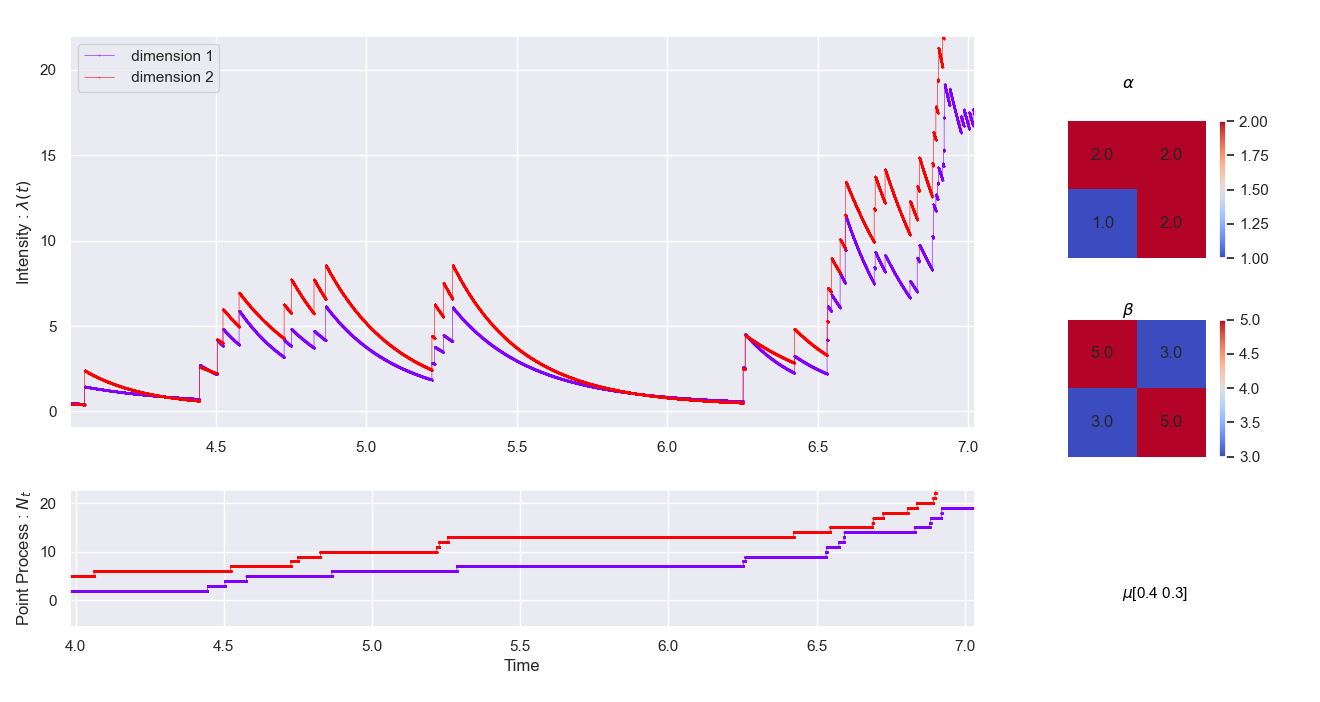
\includegraphics[width = 0.99 \textwidth]{../imag/chap1/hawkes2.png}
\caption{Sampled path from a bivariate Hawkes process. Top: intensity of each process. Bottom: corresponding counting process. The processes $N_t^m$ are shifted for readability. One can notice the interdependence between the two processes. For example, the first jump (from dimension 2) doesn't increase the two processes by the same value. The second jump (from dimension 1) increases the two processes by the same value.}
\label{fig:hawkes2}
\end{figure}


\subsection{Few Remarks about Hawkes Processes}
\begin{remarque}
The process should be considered cadlag. On the other hand, $\lambda^m$ is left-continuous adapted because if the conditional intensity has a discontinuity at some point, then its value should be defined by its history, not by the point itself (cf. \cite{daley}). Since left-continuity of the path implies predictability we use this sufficient condition. 
\end{remarque}

\begin{remarque}
Another interesting kernel is the so-called exponential kernel of order P, that one can define as:

$$ \mu (t) = \sum_{j=1}^P \alpha_j \exp( - \beta_j t ) $$

More details in \cite{exphawkes} and in \cite{exphawkes2}.
\end{remarque}

\begin{remarque}
Another popular choice for the kernel $\mu$ is a power-law function, yielding:

$$ \lambda (t \mid \Tau_{t^-} ) = \nu + \int_{- \infty }^t \frac{ k }{ \left ( c + t - s \right ) ^p } $$

where $c,k,p > 0$. It is widely used in the seismology literature and in the social media literature.
\end{remarque}




\begin{remarque}
The Hawkes process we described is referred to as the linear Hawkes process. Defining the counting process based upon a conditional intensity function of the form:

$$ \lambda (t \mid \Tau_{t^-}) = \Psi \left ( \int_{-\infty}^t \mu(t-s) dN_s \right ) $$ where $\Psi : \R \to \R_+$, we get the so-called nonlinear Hawkes process. \\Setting $\Psi(u) = \nu_1 + u$, the function reduces to the linear case. 

We mention two works related to nonlinear Hawkes processes, that one can discover inside \cite{nonlinearHP1} and \cite{nonlinearHP2}.
\end{remarque}

\begin{remarque}
A last thing about Hawkes processes is the difference between temporal and spatio-temporal Hawkes processes. Spatiality can be incorporated with an additional function convoluting with the kernel. This theoretical domain is pretty useful for seismic studies.
\end{remarque}



\subsection{Self-Regulating Hawkes Process}
\label{section:obral}

The terms 'self-exciting'  (and by opposition 'self-regulating') can be made precise through the conditional intensity function. If an event causes the stochastic conditional intensity function to increase then the process is said to be self-exciting. Empirically, it causes temporal clustering of events. 

On the other hand, if the conditional intensity function is lowered by events, the process is called self-regulating. 

Copying an image from \cite{obral} that one can find at pages $30$ and $31$, that we display on fig. \ref{fig:obral}, we show two graphs representing a self-exciting and self-regulating processes. 

The essential difference if whether the parameters $\alpha$ are taken positive or negative. 

It however changes the model completely (on a philosophical point of view) and could interfere with the estimation process of the parameters, as the boundaries for the algorithms might have to be changed.

Such processes are not examined hereinafter.

\begin{figure}
\centering
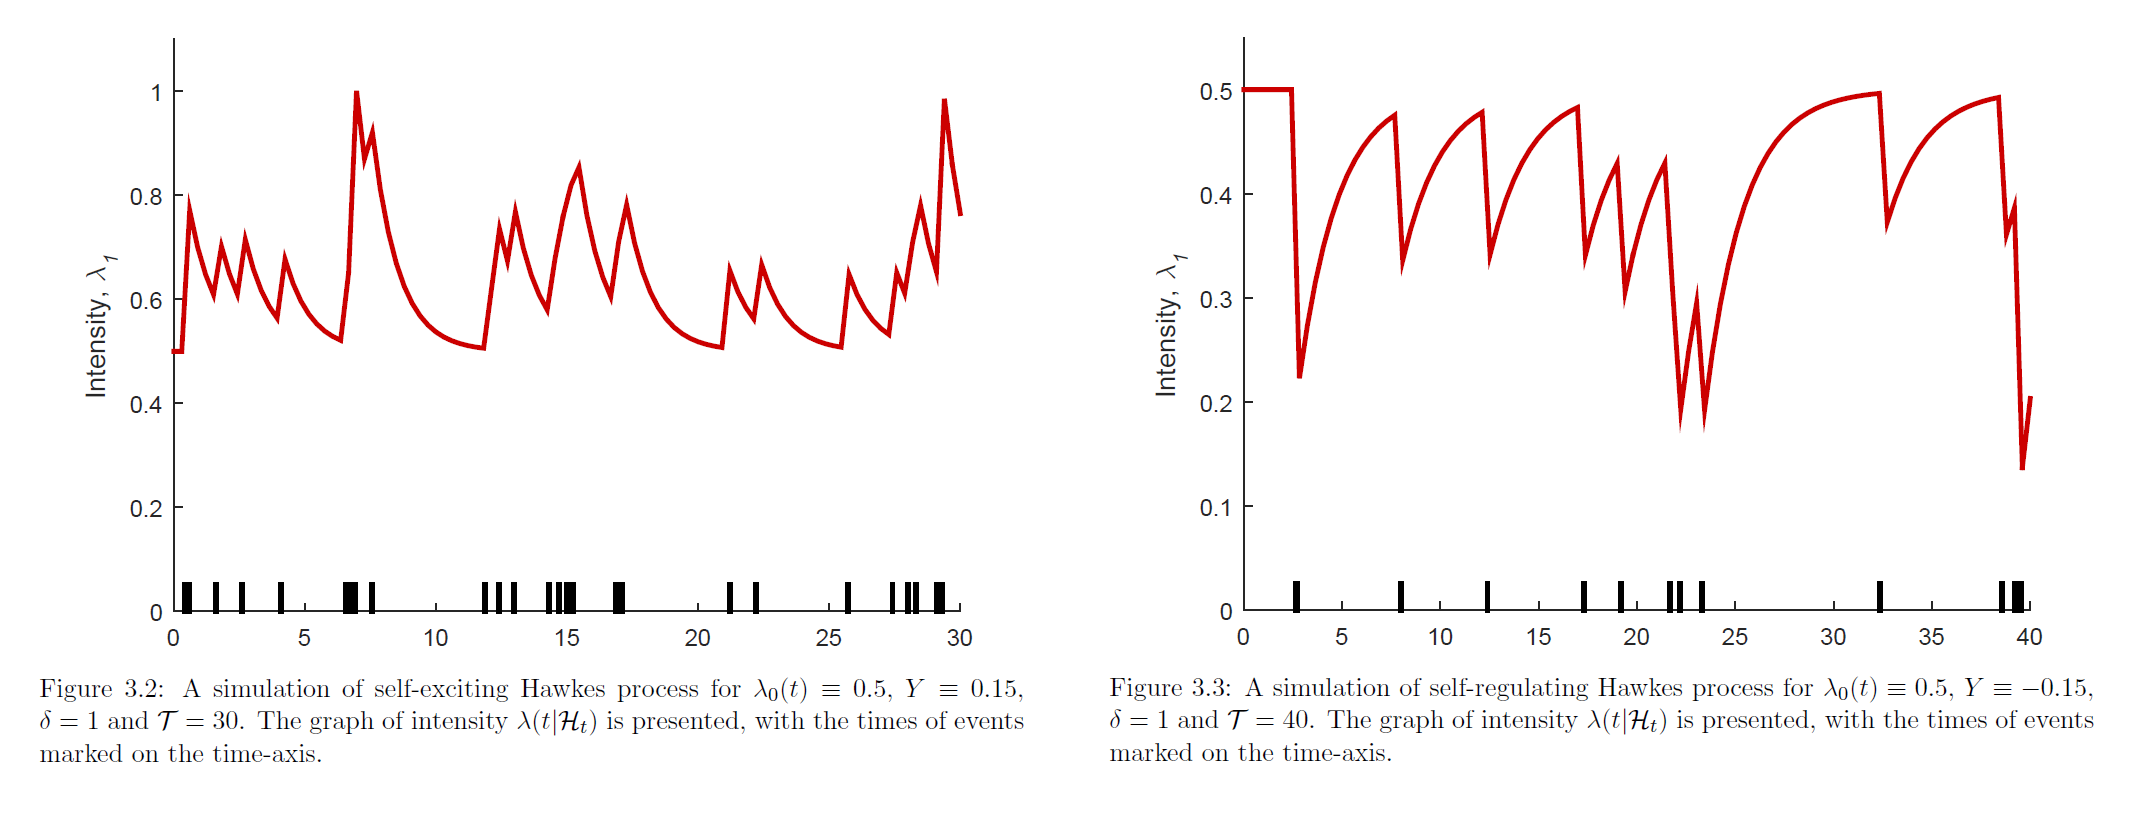
\includegraphics[width = 0.90 \textwidth]{../imag/chap1/obral.png}
\caption{ Plots of self-exciting and self-regulating processes from \cite{obral}.}
\label{fig:obral}
\end{figure}












\subsection{Hawkes Processes as Branching Structures}
We notice that Hawkes process are marked simple point processes.

Another equivalent view is its branching structure, by ignoring the time location of the events. Through the superposition
properties of point processes (cf. \cite{daley}, Theorem 2.4.VI), one can decompose the events into two categories: the immigrants and the offspring. The immigrants are the external events while the offspring is triggered by the previous events in the process. The offspring are structured into clusters associated with the original immigrant parent. That representation is particularly useful for categorizing the different Hawkes process (subcritical / critical / supercritical Hawkes process) as well as for forecast.

Essentially, the immigrants are distributed as a homogeneous Poisson process; the clusters are each associated to one immigrant and all-together form an independent partition of all the immigrants. The number of offspring is given by a Poisson law of parameter equal to the branching factor (defined below). The times of the events can be computed with the inter-arrival times, which in this case (homogeneous Poisson) are exponentially distributed.

An accessible summary about that representation is given in \cite{socialhawkes}. 

\begin{definition}[Branching Factor]
The branching factor is defined as the expected number of direct offspring spawned by a single event. For univariate, un-marked Hawkes process, the branching factor $n^*$ can be computed:

$$ n^* = \norm{ \mu }_{L^1} $$

It is fairly intuitive that when that number is greater than one, the number of immigrants might be infinite. 
\end{definition}


\begin{remarque}
A critical Hawkes process ($n^* = 1$) must not explode, though it usually does. For example, if the kernel is sufficiently long tailed, one can create a stationary Hawkes process without immigration. An example given by Brémaud and Massoulié in 2001 show that when clusters overlap while being far enough, the process might be stationary.
\end{remarque}







\subsection{Marked Hawkes Processes}
\label{subsection:marked}
A natural extension to Hawkes Processes is having stochastic kernels. The simplest example is marked kernels (where the mark is commonly coined $Y$ in the literature), like marked exponential kernels:

$$\mu(t- t_i^j, Y_i^j) =  Y_i^j \exp \left ( - \beta_j \cdot ( t - t_i ) \right ) $$

then the model from eq.(\ref{eq:stieltjes_integral3}) becomes:

\begin{align}
\lambda^m (t \mid \Tau_{t^-} ) &= \nu_m + \sum_{n = 1}^M \sum_{ \{k: t_k^n < t \}} \mu(t- t_k^{n}, Y_k^{m,n}) \notag \\
&=  \nu_m + \sum_{n = 1}^M \sum_{ \{k: t_k^n < t \}}   Y_k^{m,n} e^{- \beta_{m,n} \cdot ( t - t_k^n ) } 
\end{align}

It is a classical practice considering unpredictable marks. 



\subsection{Stability of Hawkes Processes}

\willdo{ How Hawkes is stat. conditions, 1D et multi dim ? est ce que algo fonctionne quand même? }

An interesting question is whether a Hawkes process is stationary. It is a very important question because we want the process to be stable, and to be simulable, which would be easier when the process is stationary.

Following the ideas of \cite{Hawkes}, one can write the conditional intensity process in a matrix form:
\begin{equation}
\overline{\lambda} = \E [ \lambda(t) ] = (I - \Gamma) ^{-1}\overrightarrow{\nu}  
\end{equation}

where $ \Gamma = \norm{\mu}_{L^1} $,  $\mu$ is the chosen kernel for the Hawkes process.
 
In the case of exponential kernels, $\Gamma$ takes a simple form:

\begin{equation}
\forall m,n \in \llbracket 1, M \rrbracket^2: \  \mu_{m,n} (t) = \alpha_{m,n} \exp ( - \beta_{m,n} t ) \implies \Gamma = \left ( \frac{ \alpha_{m,n} } { \beta_{m,n} } \right )_{ m,n \in \llbracket 1, M \rrbracket^2} 
\end{equation}

A sufficient condition for stationarity of the process is the spectral radius of $\Gamma$ is strictly less than 1. This is due to the fact that since the immigrant process is stationary, all we need is that the mean cluster size to be finite. Recall that the spectral radius of the matrix $\Gamma$ is defined as the maximal value of the set of the absolute eigenvalues of $\Gamma$.

In the case of marked Hawkes processes, the matrix $\Gamma$ has a slightly different form. We follow the computations from \cite{my_algo_simul}.

\willdo{ici !!! à écrire; suivre 22.}


\section{Simulation for Fixed Parameters}
\subsection{Notations}

The author refers to paper \cite{my_algo_simul} for an interesting solution in order to simulate Hawkes processes. There are different easier ways to simulate a Hawkes process (cf. appendix \ref{appendix_simulate}). However, they do not give as much flexibility as the one from \cite{my_algo_simul} and that's the reason why we use it. It is in fact, even more general than what we need. The algorithm allows the simulation of Marked Multidimensional Hawkes processes. We focus on marks being deterministic (thus we can assume that the parameters are constant).


The algorithm is the following. It is based on the idea that one can simulate the waiting time between jumps. For a $M$-dimensional process, each dimension has an impact on the other. Hence, we can simulate the waiting time for every dimension influencing every other dimension (including itself).




\begin{itemize}
\item $r_j$ is the time of the $j$-th jump and $r_0$ is by convention $0$. We define the vector $\overrightarrow{r} = \sequence{r_i}$ as being the sorted times for all events in the Hawkes processes. 
\item we also define $\overrightarrow{t}^m = \sequence{ t_i^m } $ as being the jumps' time for one marginal process. Clearly, there is the following relationship between $\overrightarrow{r}$ and $\overrightarrow{t}^m $:
$$ r = \bigcup_m \bigcup_k  t_k^m $$
\item $a_{m,j}^i$ reads the waiting time after jump $(j-1)$-th and the jump created by process $i$ upon process $m$ (thus corresponding to intensity $ \lambda^i_m$). In other words, the $i$ index indicates which dimension is triggering the jump, the $m$ index corresponds to the dimension which receives the jumps. This decomposition of the intensity is the rational of the followability of the algorithm, as defined in section \ref{section:definition_algo}.


\begin{remarque}
$$\forall m,j \in  \llbracket 1, M \rrbracket, \qquad a_{m,j}^i \sim \mathcal L_{m,j}^i   $$
Where $\mathcal L_{m,j}^i $ is defined by the CDF:
\begin{align}
F(s) &= 1 - \exp \left ( - \int_{r_{j-1}}^{r_{j-1} + s } \lambda_m^i (t) dt \right ) \notag \\
&= 1 - \exp \left ( - \frac { \lambda^i_m ( r_{j-1} ) } { \beta_m^i } ( 1 - e^{ - \beta_m^i s} ) \right )
\label{eq:L_defined}
\end{align}

Hence, we can use the inverse CDF method. It consists in inverting the previous CDF and generating a uniform random variable. The process is described in algorithm \ref{algo:CDF_1}.
\end{remarque}



\begin{algorithm}[H]
\label{algo:CDF_1}
\SetAlgoLined
$u \sim U(0,1)$,

\eIf{ $u < 1 - \exp \left ( - \frac { \lambda^i_m ( r_{j-1} ) } { \beta_m^i } \right ) $ }{
we let 
\begin{equation}
a_{m,j}^i = - \frac{1} { \beta_m^i} \ln \left ( 1 + \frac{ \beta_m^i } { \lambda^i_m ( r_{j+1} ) } \ln ( 1 - u ) \right )
\label{eq:cdf_invert}
\end{equation}
}
{$ a ^i_{m,j} = \infty $.}
\caption{Generate the waiting time of the self-exciting part.}
\end{algorithm}


Notice that there is a typo in the original document. The good formula is the one written above\footnote{One can compare the previous line (eq. \ref{eq:cdf_invert}) with the equation (20) from \cite{my_algo_simul}.}.

Also notice that the CDF defines a defective random variable ( as defined in \cite{my_algo_simul}). It means the random variable has a probability mass at $\infty$. Indeed:

$$ \mathbb P ( a^i_{m,j} = \infty ) = \exp \left ( - \frac { \lambda^i_m ( r_{j-1} ) } { \beta_m^i } \right ) > 0 $$



\item $a_{m,j}^0$ is the waiting time for the natural immigration process upon process $m$, meaning the process without the self-excitement part. 

\begin{remarque}
In order to sample $a^0_{m,j}$,
$$\forall m,j \in  \llbracket 1, M \rrbracket, \qquad a_{m,j}^0 \sim \exp( \nu_m )$$
Hence, we can use the inverse CDF method. 
\end{remarque}

\item $N^{m} (t) $ the counting process, underlying the marginal $m$-th Hawkes process, at time $t$.
\end{itemize}


Finally, one should know that the update rule for the intensity cache is given as follows, where:

\begin{equation}
\lambda_m^i ( r_j ) = \lambda_m^i ( r_{j-1} )  e^{ - \beta_m^i \min_{m,i} a_{m,j}^i } + \alpha_{i,m} \11charac_{i = m^*}
\label{eq:update_lambda} 
\end{equation}

Notice that by adjusting this expression, one can easily get the plot of the intensity of a Hawkes process:

\begin{equation}
\label{eq:update_lambda_plot} 
\forall t \in ]r_{j-1}, r_j ], \quad \lambda (t)_m^i = \lambda_m^i ( r_{j-1} )  e^{ - \beta_m^i ( t - r_{j-1} }
\end{equation} 

where we excluded the left bound because the process is left continuous.
 
With all those notations, we are ready to introduce the algorithm \ref{algo:simul_hp} in the following section.









\subsection{Algorithm for Fixed Parameters}



\begin{algorithm}[H]
\label{algo:simul_hp}
\SetAlgoLined

\For{ $j > 0$ }
			{ \While {$r_j < T$}
					{\For{$m \in \llbracket 1, M \rrbracket$}
						{Sample $a_{m,j}^0 \sim \exp( \nu_m ) $,
						
						\For{$i \in \llbracket 1, M \rrbracket$}
							{Sample $a_{m,j}^i \sim  \mathcal L^i_{m,j} $, as defined by \ref{eq:L_defined},
							}
						}
						
						$r_j = r_{j-1} + \min_{m,i} a_{m,j}^i$,
						
						\For{$m \in \llbracket 1, M \rrbracket$}
							{Update $\lambda_m^i ( r_j )$ according to equation (\ref{eq:update_lambda}),
							
							Update $N^m ( r_j ) = N^m( r_{j-1} ) + {\11charac}_{m = m^*} $,}
					$t_k^{m^*} = r_j$ where $k = N^{m^*} ( r_j ) $ and $ m^*,i^* = \argmin_{i,m} a_{m,j}^i $,
					}
			Discard the last $r_j$ > T.
			}
\caption{Exact simulation of multidimensional Hawkes process}
\end{algorithm}



\begin{remarque}
As illustration, $i^* = 0$ then $r_j$ is an immigrant; $m^* = i^*$ implies that the jump arises from self-excitation; otherwise, $r_j$ is caused by an external process $i^*$.
\end{remarque}

\begin{remarque}
Notice that the algorithm also works for $\alpha_{m,n} < 0$. One should however be cautious of not having a strictly negative intensity. Also, $\alpha_{m,n}$ can be potentially replaced by a random variable transforming the point process into a marked point process (more details in the original paper \cite{my_algo_simul}).
\end{remarque}

We can observe a sample path for a uni-variate and penta-variate Hawkes process in the following figures: \ref{fig:hawkes1} and \ref{fig:hawkes5}.

\begin{figure}
\centering
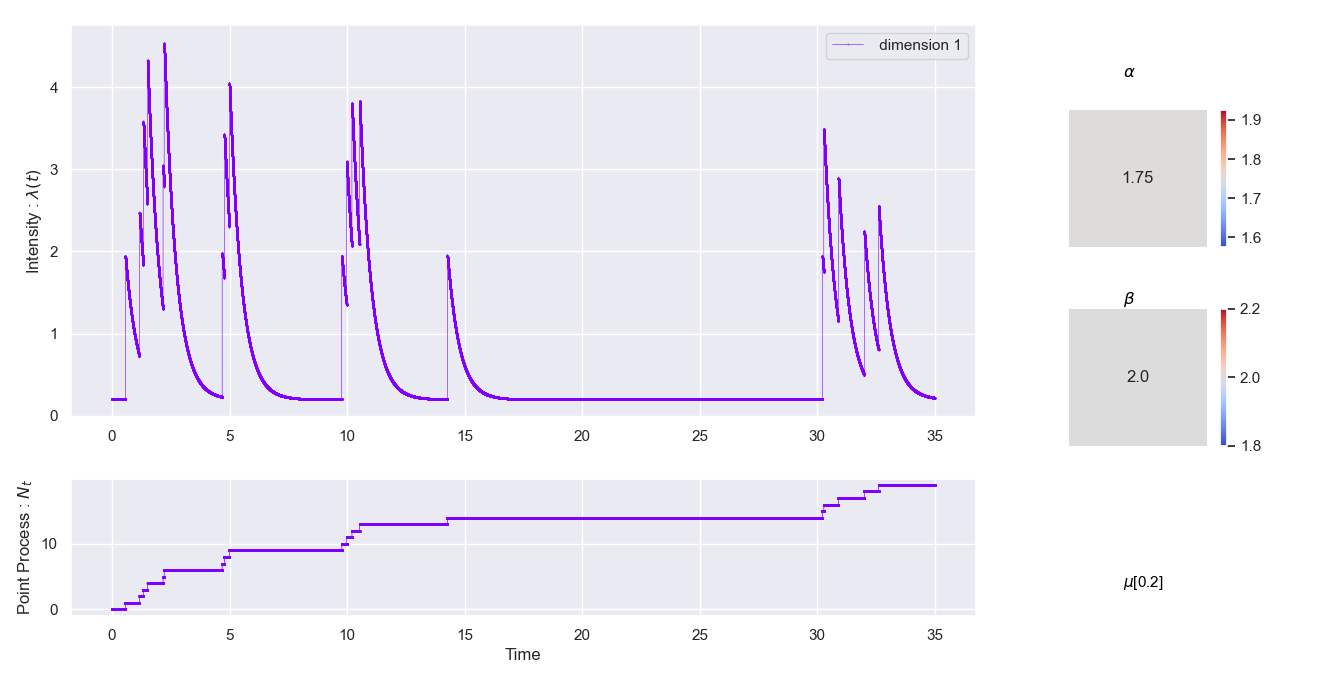
\includegraphics[width = 0.99 \textwidth]{../imag/chap1/hawkes1.png}
\caption{Sampled path from a uni-variate Hawkes process. One can easily distinguish the clusters.}
\label{fig:hawkes1}
\end{figure}


\begin{figure}
\centering
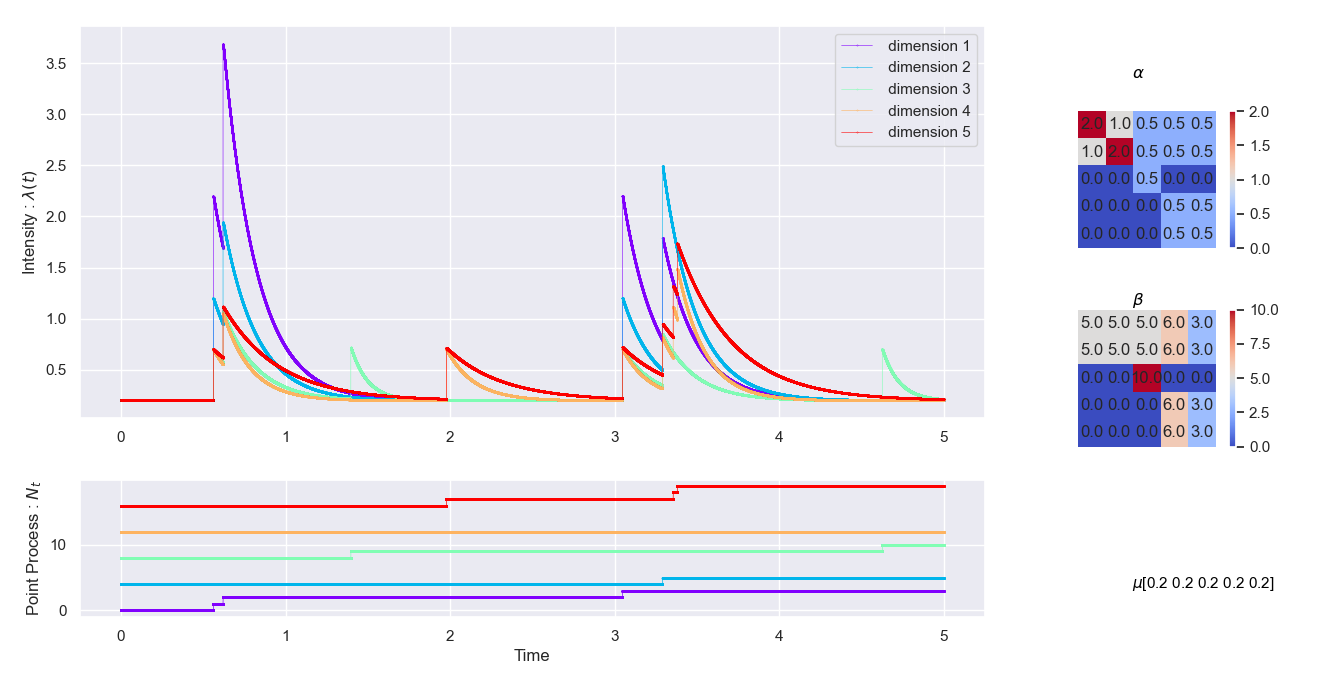
\includegraphics[width = 0.99 \textwidth]{../imag/chap1/hawkes5.png}
\caption{Sampled path from a penta-variate Hawkes process. Top: intensity of each process. Bottom: corresponding counting process. The processes $N_t^m$ are shifted for readability.}
\label{fig:hawkes5}
\end{figure}

\subsection{Edge Effect}
\label{subsection:edge}
Edge effect is defined in \cite{socialhawkes} in the following manner:

\textit{In practical applications, the process might have started sometime in the past, prior to the moment when we start observing it, denoted as $t = 0$. Hence, there may be unobserved event times which occurred before time $0$, which could have generated offspring events during the interval $[0;T]$. It is possible that the unobserved event times could have had an impact during the observation period, i.e. sometime after $t > 0$, but because we are not aware of them, their contribution to the event intensity is not recorded.}


Some interesting discussions can be found in \cite{daley}, as well as in these two papers that directly refer to edge effect: \cite{cox}, \cite{rasmussen}. The proposed methods could potentially be added to any other algorithm summarized in table \ref{table:methods_HP}.



\willprecise{understand if it is the same thing as burn in and talk about it}

\section{Simulation for Time-Dependent Parameters}
\subsection{Preliminary}

The algorithm from \cite{my_algo_simul} allows to simulate multidimensional Hawkes processes, with different decays parameters, for an exponential kernels with marks, and constant immigration rates. From that, it is obvious that one can use the previous algorithm with deterministic jumps ($\alpha$). On the other hand, the underlying intensity ($\nu$) is easily changeable by using any method for simulation non-homogeneous Poisson process.

However, the task is way harder concerning the decays ($\beta$).

To sum-up:
\begin{itemize}
\item deterministic $\alpha$ is already included in the previous algorithm.
\item deterministic $\beta$??????  The task with beta is quite harder. A usual choice is a parameter piecewise constant. 
\item deterministic $\nu$ needs some work. We are using a basic and classical thinning algorithm for that. One can find more about it in appendix part \ref{subsection:thinning}.
\end{itemize}




\willprecise{talk about the betas it with Ed}

It would also be possible to compute the CDF of the interarrival times related to a function $\nu(t)$ and inverse the formula. However, such approach makes it compulsory to solve equations by hand in order to find the inverse. The inverse can be more or less challenging to find. 


\begin{theoreme}{Non-homogeneous Poisson process interarrival times}
If the process has intensity $\nu(t)$, one gets that the pdf of the $n$-th jump's time is 

$$
f_n(t)  = \frac {\left ( \int_0^t \nu(s) ds \right )^{n-1}}{(n-1)!} \nu(t) e^{-  \int_0^t \nu(s) ds }
$$

Then the CDF for the $n$-th jump's time is:

$$
F_1(t) = 1 - e^{  \int_0^t \nu(s) ds } 
$$

\end{theoreme}

\willdo{finish the proof}

\begin{demo}{}{}
First recall that by definition of Poisson process with rate $\lambda$, one has:
$$
\mathbb P(N_t = k) = \frac { (\lambda t)^k \exp(- \lambda t ) }{k !}$$

Non-homogeneous Poisson process can be seen as a homogeneous Poisson process with a non-constant intensity function $\lambda (t)$. It can be proven (cf. \cite{Veraart}), that we also have the previous formula for non-homogeneous Poisson processes, meaning:

$$
\mathbb P(N_t = k) = \frac { \left ( \int_0^t \lambda(s) ds \right )^k \exp \left ( - \int_0^t \lambda(s) ds \right )  }{k !}$$

then from \begin{verbatim}
https://www.randomservices.org/random/poisson/
Nonhomogeneous.html
\end{verbatim}

Using the identity from theorem \ref{thrm:point_counting}.

$$ P( N_t \geq n ) = \sum_n^{\infty} \exp \left ( - \int_0^t \nu(s) ds \right ) \frac{ \left ( \int_0^t \nu(s) ds \right ) ^k }{k !} 
$$
\end{demo}


\begin{ajoutationV}{}{}
If one searches the inverse of a function of the following form:

$$ y(x) = 1 - \exp ( - (\alpha x + \beta x^2) ) $$

we get:

$$ x(y) = \frac{- \alpha \pm \sqrt{\alpha^2 - 4 \beta \ln(1-y) }  }{2 \beta}$$

Whenever $r_j$ is the time location of the jump, $s$ the time-location after $r_j$ when the next jump occurs. Replacing $$\alpha s + \beta s^2 = ( b + a r_j ) s + \frac 1 2 a s^2 $$ 
we get back to the scenario $$ \nu(t) =  a t + b $$ which is one of the four models we considered in fig. \ref{fig:evol_functions}.
\end{ajoutationV}


\subsection{Algorithm for Time-Dependent Parameters}

In order to simulate the underlying non-homogeneous Poisson process, we define the following law:
$$ \forall m,j \in  \llbracket 1, M \rrbracket, \qquad a_{m,j}^0 \sim \mathcal J_m  $$

Where $\mathcal J_m $ is defined by the CDF:
\begin{equation}
\label{eq:J_defined}
F(s) = 1 - \exp \left ( - \int_{r_{j-1}}^{r_{j-1} + s } \nu_m (t) dt \right )
\end{equation}

We also need the following equation, which deals with the deterministic $\alpha$\footnote{The only difference is that now we consider $\alpha$ as a function of the time.}:

\begin{equation}
\lambda_m^i ( r_j ) = \lambda_m^i ( r_{j-1} )  e^{ - \beta_m^i \min_{m,i} a_{m,j}^i } + \alpha_{i,m} (r_j) \11charac_{i = m^*}
\label{eq:update_lambda_time} 
\end{equation}




\begin{algorithm}[H]
\label{algo:simul_hp_time}
\SetAlgoLined

\For{ $j > 0$ }
			{ \While {$r_j < T$}
					{\For{$m \in \llbracket 1, M \rrbracket$}
						{Sample $a_{m,j}^0 \sim \mathcal J_{m} $ as defined by \ref{eq:J_defined} using a thinning algorithm (cf. algorithm \ref{algo:thinning_algo} in appendix),
						
						\For{$i \in \llbracket 1, M \rrbracket$}
							{Sample $a_{m,j}^i \sim  \mathcal L^i_{m,j} $, as defined by \ref{eq:L_defined},
							}
						}
						
						$r_j = r_{j-1} + \min_{m,i} a_{m,j}^i$,
						
						\For{$m \in \llbracket 1, M \rrbracket$}
							{Update $\lambda_m^i ( r_j )$ according to equation (\ref{eq:update_lambda_time}),
							
							Update $N^m ( r_j ) = N^m( r_{j-1} ) + {\11charac}_{m = m^*} $,}
					$t_k^{m^*} = r_j$ where $k = N^{m^*} ( r_j ) $ and $ m^*,i^* = \argmin_{i,m} a_{m,j}^i $,
					}
			Discard the last $r_j$ > T.
			}
\caption{Exact simulation of multidimensional Hawkes process}
\end{algorithm}


\vspace{0.5cm}

One can see a few example of realized univariate processes where the parameters change over time in fig. \ref{fig:param_dep_hawkes}. 


\begin{figure}
\centering
\subfloat{{
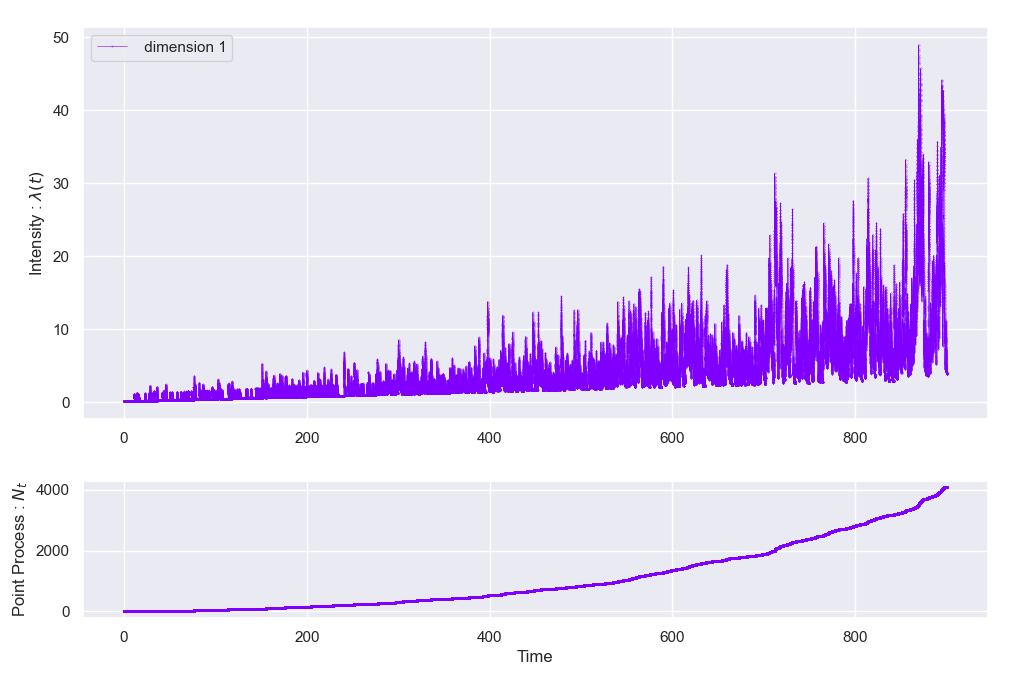
\includegraphics[width = 0.48 \textwidth]{imag/chap2/simul/Hawkes_linear.png}
}} 
\subfloat{{
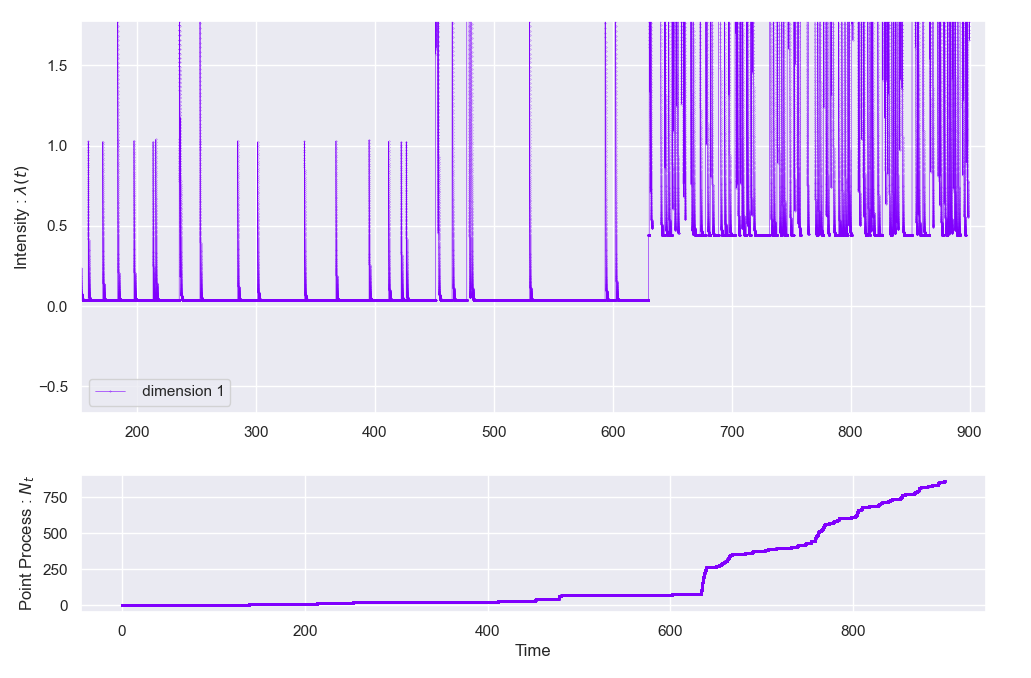
\includegraphics[width = 0.48 \textwidth]{imag/chap2/simul/Hawkes_jump.png}
}}\\
\subfloat{{
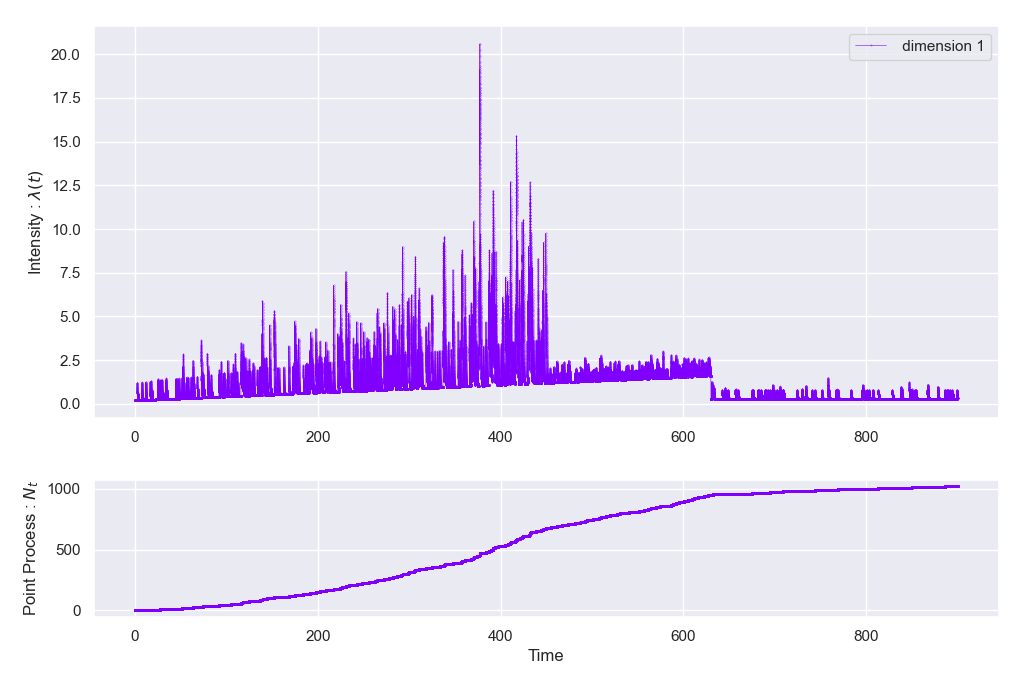
\includegraphics[width = 0.48 \textwidth]{imag/chap2/simul/Hawkes_mountain.png}
}} 
\subfloat{{
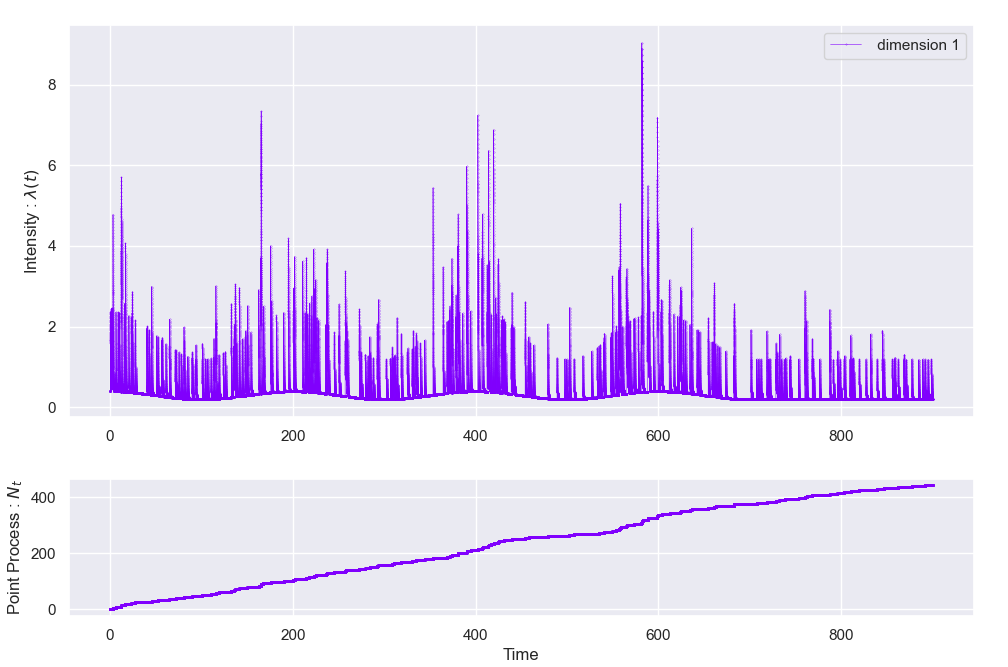
\includegraphics[width = 0.48 \textwidth]{imag/chap2/simul/Hawkes_sin.png}
}}

\caption{On the basis of the functions from fig. \ref{fig:evol_functions}, we modify $\alpha$ and $\nu$ with respect to time. One can notice the jumps, as well as the underlying intensity, changing with respect to time. For the one corresponding to "one jump" function, we zoomed in in order to emphasize the phenomena.}
\label{fig:param_dep_hawkes}
\end{figure}











\section{Our Numerical Solution}
\willdo{ talk about code?}
\subsection{Classes}
\subsection{Functions}






\part{Estimation of Hawkes' parameters}
\chapter{Introduction to Estimation}

This part investigates the problem of recovering information about data generated by Hawkes processes given by a set of parameters $\Theta = ( \nu, \alpha, \beta ) $, and for which we observe a set of jumps' times. The process can be multivariate, and we would like:

\begin{itemize}
\item to estimate the parameters $\theta$ by $\hat{\theta} = ( \hat{\nu}, \hat{\alpha}, \hat{\beta} )$. $\theta$ shall belong to a set of possible parameters, named $\Theta$.

\item to estimate the parameters with some temporal dependency on them. We then replace our estimate by: $\hat{\theta}_t$,
\item to analyze the evolution of parameters on the angle of change point analysis, and we could try to incorporate that analysis inside our estimation process, in an attempt to increase the accuracy of our estimation.
\end{itemize}


The estimators are tested over simulated data, for the sake of simplicity and lack of relevant data. Unfortunately, this method bypasses the many significant challenges raised by real datasets, challenges that caused \cite{critic_hawkes} to state that:

\textit{"Our overall conclusion is that calibrating the Hawkes process is akin to an excursion within a minefield that requires expert and careful testing before any conclusive step can be taken."}

The method considered is maximum likelihood estimation, which begins by finding the likelihood function, and estimates the model parameters as the inputs which maximise this function.

Recall that the observed information is lying in the time-interval $[0,T]$.
\chapter{Estimation : a First Approach}

\section{Introduction to Max. Likelihood Estim. (MLE)}

The Maximum Likelihood Estimator (MLE) is commonly used in order to find an estimator of the parameters. However, it has been a challenge for quite a long time, quoting \cite{daley}:

\textit{The likelihood functions for most of the processes discussed [...] are relatively intractable. This difficulty was a block to the application of general point process models until the late 1960s, when a quite different approach was introduced in papers on filtering theory pioneered by the electrical engineers. [...] Once recognised, its role in elucidating the structure of point process likelihoods was soon exploited. General definitions of the conditional intensity function were given in Rubin (1972) and especially by Brémaud (1972), in whose work conditional intensity functions were rigorously defined and applied to likelihood and other problems (see also Brémaud, 1981).}

Optimization theory (for finding maximums) is very dense, and since the log-likelihood of Hawkes processes is non-linear, we would like to use a non-linear optimization technique. 

Ozaki in \cite{Ozaki} in section 3 mentions three methods for finding the maximum likelihood

\begin{itemize}
\item Gradient and Hessian (Newton-Raphson method)
\item Gradient (Davidon's procedure)
\item Only the likelihood function (direct method)
\end{itemize}


We are going to use the Newton-Raphson method. Though it might be more expensive to compute the Hessian, it leads to better estimators.


For that purpose, we need to compute numerically the gradient and the hessian of the log-likelihood. One can find their expressions in the univariate case in Ozaki's paper (\cite{Ozaki}) but the author couldn't find any paper on the multivariate case. For that reason, we computed the algebraic expressions by hand, before putting them into code. One has to be quite careful about the code since the derivatives are very expensive to compute. We give a list of advice at the end of the chapter.





\subsection{Derivation of the Likelihood Function}
\begin{theoreme}{Likelihood of a simple point process}
From definition 7.1.II in \cite{daley}; let us say that a simple point process has list-history: $\sequence{ t_i }$, on a bounded Borel set $A$. Then, the likelihood of a process $N$ can be expressed as:
\begin{equation}
L( \theta \mid \sequence{t_i} ) =  \frac{\mathbb P \left (N_{\theta}  \text{ has } \# \sequence{t_i} \text{ points in } A \text{ at locations  } (d t_1, \cdots, d t_n) \right ) } {(d t_1, \cdots, d t_n)}
\end{equation}

Notice that since $A$ is bounded, the sequence is finite so the $\#\sequence{t_i}$ number of elements is finite too. 
\end{theoreme}




In order to have a closed form expressions for the term $$\frac{\mathbb P \left (N_{\theta}  \text{ has } \# \sequence{t_i} \text{ points in } A \text{ at locations  } (d t_1, \cdots, d t_n) \right ) } {(d t_1, \cdots, d t_n)}  =: \mathbb P ( \mathcal N_{\theta} ) $$

we introduce a function:
\begin{definition}[Conditional Survivor Functions]
\begin{equation}
\forall u \in \R, k \in \N, \qquad S_k ( u \mid t_1, \cdots, t_{k-1} ) = \mathbb P ( t_k - t_{k-1} > u \mid t_1, \cdots, t_{k-1} ) 
\end{equation}
\end{definition}



Then, one can actually prove that for every simple point process, there exists a unique family of survivor functions such that

\begin{theoreme}{Associated Survivor to a Simple Point Process}
From proposition 7.2.I in \cite{daley}; we have that there exists a unique family of conditional probability density functions $\sequence{p_i}$\footnote{Thus there exists a bijection between the families of probability density functions as described and the marked point process.} and associated survivor functions, related in the following way:
\begin{equation}
\forall 0 < t_1 < \cdots < t_{n-1} < t, \quad S_n( t \mid t_1, \cdots, t_{n-1} ) = 1 - \int_{t_{n-1}}^t p_n ( u \mid t_1, \cdots, t_{n-1} ) du
\end{equation}
Then, we have the following expression whenever $0 < t_1 < \cdots < t_{n} < T < \infty $:
\begin{equation}
\mathbb P ( \mathcal N_{\theta} )  =   \prod_{i = 1}^n p_i ( t_i \mid t_1 \cdots t_{i-1} ) \times S_{n+1} ( T \mid t_1, \cdots, t_n )  
\end{equation}
\end{theoreme}


\begin{remarque}
In layman terms, $p_n$ is the conditional probability density function of the time of the next event knowing the previous events
\end{remarque}


\begin{theoreme}[label = theoreme_expression_ln_lik]{Closed Form of the Likelihood for a Simple Point Process}
If $N$ is a simple point process on $[0,T]$,  $0 < T < \infty$, and we are aware of the realization of $N$ over $[0,T]$ as being $\sequence{t_i}$, then the likelihood $L$ of $N$ reads:
\begin{align}
L( \theta \mid \mathcal F ) &= \exp \left ( - \int_{0}^{T} \lambda_{\theta} ( s \mid \mathcal F ) ds \right )  \prod_{i=1}^{N(T)}  \lambda_{\theta} ( T_i = t_i \mid \mathcal F_{t_{i-1}^-} )  
\end{align}
\end{theoreme}


\begin{demo}{}{}
Let us assume that $N(T) = \# \sequence{ t_i } =: n$.

Given in definition \ref{def:lambda_1}, we have:
$$\lambda_{\theta}( T_n = t \mid \mathcal F_{t^-} ) = \frac{ p_n( t \mid \mathcal F_{t^-} )}{S_n( t \mid \mathcal F_{t^-} )}$$


yielding  this rough idea of inversion:

\begin{align*}
\forall i \leq n, \quad \int_{t_i}^t \lambda_{\theta}( T_i = s \mid \mathcal F_{s^-} ) ds &= - \ln ( S_i (t \mid \mathcal F_{t^-} ))  \\
& \iff \\
\forall i \leq n, \quad  S_i( t \mid \mathcal F_{t^-} ) & = 1 -  \exp \left ( - \int_{t_i}^t \lambda_{\theta} ( s \mid \mathcal F_{s^-} ) \right ) ds \\
& \qquad \text{ and } \\
\forall i \leq n, \quad  p_i( T_i = t \mid \mathcal F_{t^-} ) & = \lambda_{\theta} ( T_i = t \mid \mathcal F_{t^-} ) \\
& \times \quad \exp \left ( - \int_{t_i}^t \lambda_{\theta} ( s \mid \mathcal F_{s^-} ) \right ) ds 
\end{align*} 


We get that the likelihood can be written as:
\begin{align}
L( \theta \mid \mathcal F ) &= \prod_{i=1}^n p_i( T_i = t_i \mid \mathcal F_{t_{i-1}} ) \times S_{n+1} ( T \mid t_1, \cdots, t_n ) \notag \\
&=  \prod_{i=1}^n  \lambda_{\theta} ( T_i = t_i \mid \mathcal F_{t_i^-} ) \exp \left ( - \int_{t_{i-1}}^{t_{i}} \lambda_{\theta} ( s \mid \mathcal F_{t_i} ) ds \right ) \notag \\
 & \qquad \times \exp \left ( - \int_{t_n}^T \lambda_{\theta} ( s \mid \mathcal F_{t_n} ) ds \right ) \notag \\
&=  \exp \left ( - \int_{0}^{T} \lambda_{\theta} ( s \mid \mathcal F ) ds \right )  \prod_{i=1}^n  \lambda_{\theta} ( T_i = t_i \mid \mathcal F_{t_{i-1}^-} )   
\end{align}
\end{demo}{}{}













\subsection{Theory of MLE}
We derived an expression for the likelihood in the previous subsection (recall theorem \ref{theoreme_expression_ln_lik}). 

Directly, we derive the log-likelihood of a simple point process, for which one knows the conditional intensity function $\lambda$. It reads:

\begin{align}
\ln L( \theta \mid \Tau, \lambda ) &= - \int_0^T  \lambda(s \mid \mathcal F_{s^-}) ds + \int_0^T  \ln \lambda(s \mid \mathcal F_{s^-} )d N_s \notag \\
&=  - \int_0^T \lambda(s \mid \mathcal F_{s^-}) ds + \int_0^T  \ln \lambda(s \mid \mathcal F_{s^-} )d N_s 
\label{eq:intensity_lambda}
\end{align}

We highlight the presence of the integral of the conditional intensity function over time, which is known as the compensator of the point process, relative to some given history $\mathcal F$. 


\begin{definition}[Compensator]
\label{def:compensator}
For a counting process $N$ we define the function $$\Lambda(t) = \int_0^t \lambda (s \mid \mathcal F_{s^-} ) ds $$  to be the compensator of the counting process.
\end{definition}

That quantity has actually some meaningful properties,

\begin{theoreme}{Compensator as the Drift Part of a Martingale}
Assume that N is $\mathcal F$-adapted and admits a left-continuous conditional intensity $\lambda$. Then the process $M(t) = N(t) - \Lambda (t)$ is a $\mathcal F$ martingale, i.e.:

$$\forall 0 < t < s, \E [ M(s) \mid \mathcal F_t ] = M(t)$$
\end{theoreme}


\begin{demo}{}{}
Some intuition behind that theorem is given in \cite{daley}.

Intuitively, $\E[M(s) \mid \mathcal F_t]$ is constant because, for a small increment $\Delta$:

\begin{align*}
\E \left [ M( t + \Delta ) - M(t) \right ] &= \E \left[ N(t+ \Delta ) - N(t) - \Lambda( t + \Delta) + \Lambda(t) \mid \mathcal F_t \right ] \\
&\approx   \E \left[ N(t+ \Delta ) - N(t) \mid \mathcal F_t \right ] - \lambda(t) \Delta  \\
&\approx \left ( \lambda(t) - \lambda(t) \right  ) \Delta  \\
&= 0 
\end{align*}
In other words, the compensator is centring the counting process around zero: 

$$\E [ N^m (t) - N^m (0) ] = \E  \left  [ \E [ N^m (t) - N^m (0) \mid \Lambda_m(t) ]  \right ] = \E [ \Lambda_m (t) ] $$

\end{demo}

Actually, the decomposition of the process into the compensator and a martingale comes from the Doob-Mayer decomposition. A very common technique when looking at general stochastic processes is to break them down into separate martingale and drift terms. 

This is easiest to describe in the discrete time situation. So, suppose that the process $\sequence{X_i}$  is a stochastic process adapted to the discrete-time filtered probability space  $(\Omega, \mathcal F, \mathcal F_n, \mathbb P )$. If $X$ is integrable, then it is possible to decompose it into the sum of a martingale $M$ and a process $\Lambda$, starting from zero, and such that $\Lambda_n$ is $\mathcal{F}_{n-1}$-measurable for each $n\ge1$. That is, $\Lambda$ is a predictable process. The martingale condition on $M$ enforces the identity:

\begin{equation}
\Lambda_n-\Lambda_{n-1}={\mathbb E}[\Lambda_n-\Lambda_{n-1}\vert\mathcal{F}_{n-1}]={\mathbb E}[X_n-X_{n-1}\vert\mathcal{F}_{n-1}]
\end{equation}

So, $\Lambda$ is uniquely defined by
\begin{equation}
\Lambda_n=\sum_{k=1}^n{\mathbb E}\left[X_k-X_{k-1}\vert\mathcal{F}_{k-1}\right]
\end{equation}

and is referred to as the compensator of $X$. Essentially, it is the predictable term in the Doob decomposition.


In continuous time, where we work with respect to a complete, as well as, filtered probability space $(\Omega,\mathcal{F},\{\mathcal{F}_t\}_{t\ge0},{\mathbb P})$, the situation is much more complicated. There is no simple explicit formula for the compensator of a process. Instead, it is defined as follows.

Under regularity condition of the adapted process (finite variation and cadlag), the compensator $\Lambda $ is defined with $\Lambda_0=0$, such that $X-\Lambda$ is a local martingale. 


\begin{theoreme}{Existence of Compensator}
The processes for which a compensator exists are precisely the special semimartingales or, equivalently, the locally integrable semimartingales. 
\end{theoreme}

In particular, all continuous and adapted processes are predictable but, due to the existence of continuous martingales such as Brownian motion, this means that decompositions as sums of martingales and predictable processes are not unique. It is therefore necessary to impose further conditions on the term $\Lambda$ in the decomposition. It turns out that we obtain unique decompositions if, in addition to being predictable, $\Lambda$ is required to be cadlag with locally finite variation. 

One can prove that both definition (Doob-Meyer decomposition and definition \ref{def:compensator}) agree.

Recall from eq. (\ref{eq:stieltjes_integral3}), the conditional intensity for a $M$-multivariate Hawkes process reads:

\begin{align}
\lambda^{m} (t \mid \Tau_{t^-} ) &= 
\nu_m + \sum_{n = 1}^M \sum_{ \{k: t_k^n < t \}} \alpha_{m,n} e^{- \beta_{m,n} \cdot ( t - t_k^n ) } 
\end{align}


Then we can write the compensator for a multivariate Hawkes process as:

\begin{align}
\Lambda^{m}(T) &= - \int_0^T \left [ \nu_m + \sum_{n = 1}^M \sum_{ \{k: t_k^n < t \}} \alpha_{m,n} e^{- \beta_{m,n} \cdot ( t - t_k^n ) } \right ] dt \notag \\
&=  - \int_0^T \nu_m dt  + \sum_{n = 1}^M  \int_0^T \sum_{ \{k: t_k^n < t \}} \alpha_{m,n} e^{- \beta_{m,n} \cdot ( t - t_k^n ) } dt
\label{eq:compensator}
\end{align}

which, when the parameters are constant with respect to time, reduces to:

\begin{align}
\Lambda^{m}(T) = - \nu_m T  - \sum_{n = 1}^M  \frac{\alpha_{m,n}}{ \beta_{m,n} } \sum_{ \{k: t_k^n < T \}} \left ( 1 - e^{- \beta_{m,n} \cdot ( T - t_k^n ) }  \right ) 
\label{eq:compensator_constant}
\end{align}

We then use the expression of the conditional intensity and the compensator inside the log-likelihood, i.e. equations (\ref{eq:stieltjes_integral3}) and (\ref{eq:compensator}) inside (eq. \ref{eq:intensity_lambda}). We get:


\begin{align}
\ln L( \theta \mid \Tau, \lambda^{m} ) &=  T - \int_0^T \lambda^m(t \mid \mathcal F_{t^-}) ds + \int_0^T  \ln \lambda^{m}(t \mid \mathcal F_{t^-} )d N_t  \notag \\
&= T - \Lambda^{m}(T) + \sum_{i=1}^n  \ln \lambda^{m}(t_i \mid \mathcal F_{t_i^-} ) \notag \\
&= 
T - \int_0^T \nu_m dt  + \sum_{n = 1}^M  \int_0^T \sum_{ \{k: t_k^n < t \}}  \alpha_{m,n} e^{- \beta_{m,n} \cdot ( t - t_k^n ) } dt \notag
\\ &  \qquad + \sum_{i=1}^n  \ln \left ( 
\nu_m + \sum_{n = 1}^M \sum_{ \{k: t_k^n < T \}} \alpha_{m,n} e^{- \beta_{m,n} \cdot ( T - t_k^n ) }
\right ) 
\end{align}

which in the case of constant parameters, reduces to:

\begin{theoreme}[label = thrm:ln-like]{Log Likelihood: $M$-variate Hawkes with constant parameters}
\begin{align}
\ln L( \theta \mid \Tau, \lambda^{m} ) &= - \nu_m T  - \sum_{n = 1}^M \frac{\alpha_{m,n}}{ \beta_{m,n} } \sum_{ \{k: t_k^n < T \}} \left ( 1 - e^{- \beta_{m,n} \cdot ( T - t_k^n ) }  \right )  \notag
\\ & \quad \qquad + \sum_{i=1}^n  \ln \left ( 
\nu_m + \sum_{n = 1}^M \sum_{ \{k: t_k^n < T \}} \alpha_{m,n} e^{- \beta_{m,n} \cdot ( T - t_k^n ) }
\right ) 
\end{align}
\end{theoreme}







\section{Algorithm for Estimation}
With the expression of the likelihood for a Hawkes Process, it is now possible to find the MLE. We use a classic multivariate Newton-Raphson algorithm. 

\subsection{Multivariate Newton Raphson Algorithm}
For the sake of completeness, we include the basic idea behind a multivariate Newton Raphson algorithm. 


\willdo{ i have that to write} 

\begin{theoreme}{Step of the Multivariate Newton Raphson Algorithm}
One iteration of the algorithm corresponds to do...
\end{theoreme}

\subsection{Implementation and Optimization}
\label{subsection:challenge}
It can be quite challenging to use this algorithm for Hawkes Processes. First, there is a computational bottleneck due to the computation of the expressions of $R, R', R''$, defined in subsection \ref{subsection_R_def} and that appears in the computations of the log-likelihood. There is unfortunately, up-to-now, no recursive formulas for $R'$ and $R''$. 

We show the mean time required for simulating and applying the Newton-Raphson algorithm to one process, while changing the number of jumps of the process. The fig. \ref{fig:complex} displays a quadratic tendency. The usage of the profiler shows that most of the computations come from the bottleneck.  

\begin{figure}
\centering
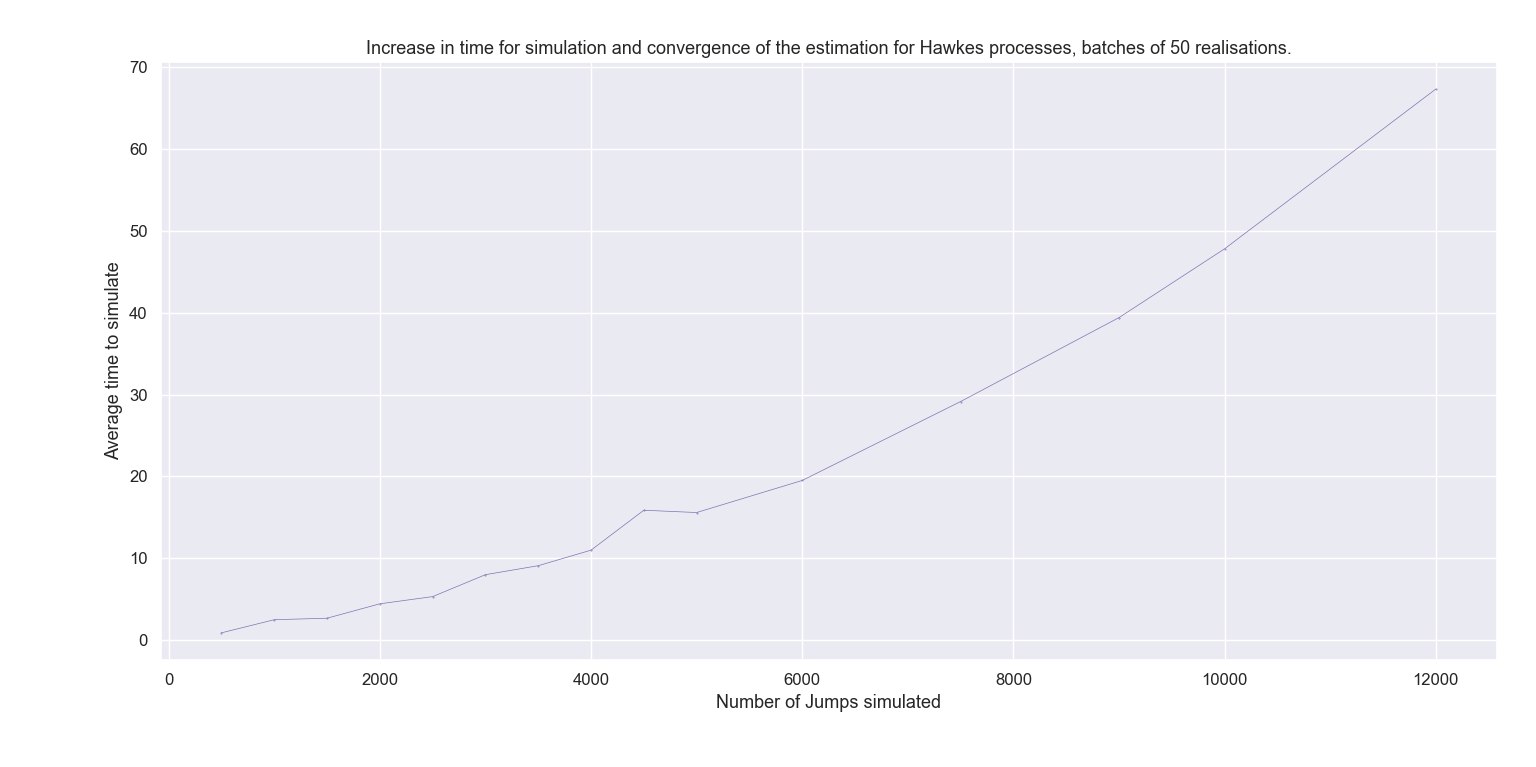
\includegraphics[width = 0.90 \textwidth]{../imag/chap2/complexity.png}
\caption{Time in seconds in order to simulate and estimate one Hawkes Process. The plot shows a quadratic trend for the complexity.}
\label{fig:complex}
\end{figure}

Another issue while using the Newton-Raphson is the neither regular nor convex nature of the derivatives. This leads to the existence of numerous local maxima of the log-likelihood. Hence, the result of an estimation might be a local maxima instead of the desired global maxima. For that reason, a usual technique for checking is using a few different initial conditions or using another searching method.















\section{Numerical Required Computations}
\subsection{Gradient and Hessian's values}
\label{subsection_R_def}

We found out in theorem \ref{thrm:ln-like} that the log-likelihood of a Hawkes process with exponential decay has a closed form. What about the multivariate likelihood?

\vspace{0.6 cm}
\underline{\textbf{Likelihood Function}}

Likelihood function of the multivariate Hawkes process is given by:

\begin{equation}
\ln L( \theta \mid \Tau ) = \sum_{m = 1}^M \ln L^m( \theta \mid \Tau )
\label{eq:ln_multi}
\end{equation}

This follows from the previous theorem \ref{thrm:ln-like}. A more detailed explanation is given in \cite{Likelihood_Hawkes}.



We fix $m,n$ as being inside $\llbracket 1, M \rrbracket ^2 $. Also notice that the $m$-th likelihood is only influenced by a subset of the parameters:

\begin{align*}
\forall m \in \llbracket 1, M \rrbracket , \  \ln L^m( \theta \mid \Tau ) &= \ln L^m( 
\{ \nu_i \}_{ i \in  \llbracket 1, M \rrbracket  },
\{ \alpha_{i,j} \} _{ i,j \in  \llbracket 1, M \rrbracket ^2 },
\{ \beta_{i,j} \}_{ i,j \in  \llbracket 1, M \rrbracket ^2 }
\mid \Tau ) \\
&= \ln L^m( 
\{ \nu_m \},
\{ \alpha_{m,j} \} _{ j \in  \llbracket 1, M \rrbracket  },
\{ \beta_{m,j} \}_{j \in  \llbracket 1, M \rrbracket  }
\mid \Tau )
\end{align*}

In other words, the gradient simplifies to its corresponding marginal gradient. 

Then, we introduce the function $R$ inside theorem \ref{thrm:ln-like}. The log-likelihood reads:


\begin{align}
\ln L^m( \theta \mid \Tau ) = - \nu_m T &- \sum^p_{n=1} \frac {\alpha_{m,n} } {\beta_{m,n}}  \lsum{n} (1 - \lexp{n}) \notag \\ 
&+ \lsum{m} \ln \left ( \denomR \right ) 
\end{align}

where $R_{m,n}$ is defined as $R_{m,n}(1) = 0 $ and for $k \geq 1$ as  

\begin{equation*}
\forall k \geq 2, \qquad R_{m,n} (k) = \sum_{ \{i : t_i^n < t_k^m \} } \exp \left ( - \beta_{m,n} \cdot ( t_k^m - t_i^n )  \right ) 
\end{equation*}

We will prefer, instead of it, this recurrent expression which leads to faster computations:

\begin{align*}
k = 1, \quad R_{m,n} (k) &= 0 \\
k \geq 2, \quad R_{m,n} (k) &= \exp ( - \beta_{m,n} \cdot ( t_k^m - t^m_{k-1} ) ) R_{m,n} (k-1) \\ 
& + \sum_{ \{i: t_i^n \in [ \ t_{k-1}^m, t_k^m \ [ \  \} } \exp ( - \beta_{m,n} ( t^m_k - t_i^n ) )
\end{align*}


\begin{remarque}
Notice that it is possible to use this less expensive expression in the case $m=n$: 
$$k \geq 2, \quad R_{m,n} (k) = \exp ( - \beta_{m,n} \cdot ( t_k^m - t^m_{k-1} ) ) (1 + R_{m,n} (k-1))$$

\end{remarque}

Furthermore, we will also need the derivatives of those expression for which no useful recurrent expression exists yet. 


\begin{align*}
k = 1, \quad R'_{m,n} (k) &= 0 \\
k \geq 2, \quad R'_{m,n} (k) &= \sum_{ \{i : t_i^n < t_k^m \} } (t_k^m - t_i^n)  \exp \left ( - \beta_{m,n} \cdot ( t_k^m - t_i^n ) \right )
\end{align*}


\begin{align*}
k = 1, \quad R''_{m,n} (k) &= 0 \\
k \geq 2, \quad R''_{m,n} (k) &= \sum_{i : t_i^n < t_k^m } (t_k^m - t_i^n)^2  \exp ( - \beta_{m,n} \cdot ( t_k^m - t_i^n ) )
\end{align*}















\vspace{0.6 cm}
\underline{\textbf{First order derivatives}}
\begin{equation}
\frac{\partial } {\partial \nu_m} \ln L^m ( \theta \mid \Tau ) = - T + \lsum{m} \frac 1 {\denomR}
\end{equation}
\begin{align}
\frac{\partial  } {\partial \alpha_{m,n}} \ln L^m ( \theta \mid \Tau ) &= - \frac 1 {\beta_{m,n}} \lsum{n} ( 1 - \lexp{n} ) \notag \\ &+ \lsum{m} \frac{R_{m,n}(k)}{\denomR}
\end{align}

\begin{align}
\frac{\partial  } {\partial \beta_{m,n}} \ln L^m ( \theta \mid \Tau ) &= \frac {\alpha_{m,n}} {\beta_{m,n}^2} \lsum{n} ( 1 - \lexp{n} ) \notag \\ 
&-  \frac{ \alpha_{m,n} } { \beta_{m,n} } \lsum{n} ( T-t_k^n) \lexp{n} ) \notag \\ 
&- \lsum{m} \frac{\alpha_{m,n} R'_{m,n} (k) }{ \denomR}
\end{align}















\vspace{0.6 cm}
\underline{\textbf{Second order derivatives}}

\begin{equation}
\frac{\partial^2  } {\partial \nu_m^2} \ln L^m ( \theta \mid \Tau ) = -  \lsum{m} \frac 1 { \left (\denomR \right )^2}
\end{equation}
\begin{equation}
\frac{\partial^2 } {\partial \nu_m \partial \nu_{m'}} \ln L^m ( \theta \mid \Tau ) = 0, \qquad m \neq m'
\end{equation}


\begin{equation}
\frac{\partial^2  } {\partial \alpha_{m,n}^2} \ln L^m ( \theta \mid \Tau ) = - \lsum{m} \left [ \frac{R_{m,n}(k)}{\denomR} \right ] ^2
\end{equation}
\begin{equation}
\frac{\partial^2 } {\partial \alpha_{m,n} \partial \alpha_{m,n'} } \ln L^m ( \theta \mid \Tau ) =  - \lsum{m}  \frac{R_{m,n}(k) R_{m,n'}(k) }
{\left ( \denomR  \right ) ^2}, \qquad n \neq n'
\end{equation}
\begin{equation}
\frac{\partial^2 } {\partial \alpha_{m,n} \partial \alpha_{m',n'} } \ln L^m ( \theta \mid \Tau ) = 0 , \qquad m \neq m'; n,n' \in  \llbracket 1, M \rrbracket
\end{equation}

\begin{equation}
\frac{\partial^2 } {\partial \nu_m \partial \alpha_{m,n} } \ln L^m ( \theta \mid \Tau ) =  - \lsum{m}  \frac{R_{m,n}(k) }{  \left ( \denomR \right )^2} 
\end{equation}

\begin{equation}
\frac{\partial^2  } {\partial \nu_m \partial \alpha_{m',n} } \ln L^m ( \theta \mid \Tau ) = 0 , \qquad m \neq m', n \in  \llbracket 1, M \rrbracket
\end{equation}



\begin{align}
\frac{\partial^2 } {\partial \beta_{m,n}^2} \ln L^m ( \theta \mid \Tau ) = & - 2 \frac {\alpha_{m,n}} {\beta_{m,n}^3} \lsum{n} ( 1 - \lexp{n} ) \notag \\ 
+  2 \frac{ \alpha_{m,n} } { \beta_{m,n}^2 } & \lsum{n} ( T-t_k^n) \lexp{n} )  \notag \\
+ \frac{ \alpha_{m,n} } { \beta_{m,n} } & \lsum{n} ( T-t_k^n)^2 \lexp{n} )  \notag \\ 
+ \lsum{m} & \left (  \frac{\alpha_{m,n} R''_{m,n} (k) }{ \left ( \denomR \right )^2} - \left ( \frac{\alpha_{m,n} R'_{m,n} (k) }{ \denomR} \right )^2 \right ) 
\end{align}

\begin{equation}
\frac{\partial^2 } {\partial \beta_{m,n} \partial \beta_{m,n'} } \ln L^m ( \theta \mid \Tau ) =  - \lsum{m} \frac{\alpha_{m,n} R'_{m,n}(k) \alpha_{m,n'} R'_{m,n'}(k) }{ \left ( \denomR \right )^2}, \qquad n\neq n'
\end{equation}

\begin{equation}
\frac{\partial^2 } {\partial \beta_{m,n} \partial \beta_{m',n'} } \ln L^m ( \theta \mid \Tau ) = 0, \qquad m \neq m'; n,n' \in  \llbracket 1, M \rrbracket
\end{equation}



\begin{equation}
\frac{\partial^2 } {\partial \nu_m \partial \beta_{m,n} } \ln L^m ( \theta \mid \Tau ) = \lsum{m} \frac{\alpha_{m,n} R'_{m,n}(k)}{\left ( \denomR \right )^2}
\end{equation}

\begin{equation}
\frac{\partial^2 } {\partial \nu_m \partial \beta_{m',n} } \ln L^m ( \theta \mid \Tau ) = 0, \qquad m \neq m'; n \in  \llbracket 1, M \rrbracket
\end{equation}


\begin{align}
\frac{\partial^2 } { \partial \beta_{m,n} \partial \alpha_{m,n} }  \ln L^m ( \theta \mid \Tau ) =  & \frac {1} {\beta_{m,n}^2} \lsum{n} ( 1 - \lexp{n} ) \notag \\ 
&-  \frac{ 1 } { \beta_{m,n} } \lsum{n} ( T-t_k^n) \lexp{n} ) \notag \\ 
&- \lsum{m} \frac{ R'_{m,n} (k) }{ \denomR  } \notag \\
&+ \lsum{m} \frac{ \alpha_{m,n} R'_{m,n} (k) R_{m,n}(k) }{ \left ( \denomR \right )^2 }
\end{align}

\begin{equation}
\frac{\partial^2 } { \partial \beta_{m,n} \partial \alpha_{m,n'} } \ln L^m ( \theta \mid \Tau ) = \lsum{m} \frac{ \alpha_{m,n} R'_{m,n} (k) R_{m,n'}(k) }{ \left ( \denomR \right )^2 }, \qquad n \neq n'
\end{equation}

\begin{equation}
\frac{\partial^2 } {\partial \alpha_{m,n} \partial \beta_{m',n'} } \ln L^m ( \theta \mid \Tau ) = 0, \qquad m \neq m'; n,n' \in  \llbracket 1, M \rrbracket
\end{equation}



\subsection{Gradient and Hessian's structure}
The derivatives are obviously at least $\mathcal C^2$. Thus, by using Schwartz theorem, the gradient exists, so does the hessian and the latter is symmetric. This is pretty important because it allows to reduce the number of required computations by almost $2$. In other words, by keeping the notation from further-on, we can use, 

$$\forall i,j \in  \llbracket 1, M \rrbracket ^ 2,  H_{i,j} = H_{j,i}^T, \quad \text{and  } \forall i \in  \llbracket 1, M \rrbracket, H_{i,i} \text{ is symmetric.} $$


Hereinafter we draw a proposition for the structure of the gradient and the hessian, coined respectively by $D$ and $H$, for a M-variate Hawkes process:

\begin{equation}
D = \left ( 
\frac{\partial } {\partial \nu_1}, \cdots, \frac{\partial } {\partial \nu_M}
, 
\frac{\partial } {\partial \alpha_{1,1}},  \cdots, 
\frac{\partial } {\partial \alpha_{1,M}}, 
\frac{\partial } {\partial  \alpha_{2,1}}, \cdots, 
\frac{\partial } {\partial  \alpha_{M,M}}, 
\frac{\partial } {\partial  \beta_{1,1}}, \cdots, 
\frac{\partial } {\partial  \beta_{1,M}}, 
\frac{\partial } {\partial \beta_{2,1}}, \cdots, 
\frac{\partial } {\partial  \beta_{M,M}}  \right ) 
\end{equation}

By separating the Hessian into 9 pieces:

\begin{equation}
H = 
\begin{pmatrix}
H_{1,1} & H_{1,2}    & H_{1,3}  \\
H_{2,1}   &  H_{2,2}   & H_{2,3}\\
H_{3,1}      & H_{3,2}       &  H_{3,3}
\end{pmatrix}
\end{equation}

Where each individual piece reads, and we highlighted the groups of the same derivatives in respective colors:
\begin{equation}
H_{1,1} = 
\begin{pmatrix}
\textcolor{blue}{\frac{\partial^2 } {\partial \nu_1 \partial \nu_1 }} & 0       & \cdots & 0 & 0       \\
0      & \textcolor{blue}{\frac{\partial^2 } {\partial \nu_2 \partial \nu_2 }}
  & \cdots      &  0 & 0       \\
0      & 0       &  \textcolor{blue}{\frac{\partial^2 } {\partial \nu_3 \partial \nu_3 }}
     & \cdots & \vdots  \\
\vdots & \vdots  & \vdots & \textcolor{blue}{\ddots} & 0       \\
0      & 0       & \cdots & 0      & \textcolor{blue}{\frac{\partial^2 } {\partial \nu_M \partial \nu_M }}
\end{pmatrix}
\end{equation}

$$ H_{2,2} = $$
\begin{equation}
\begin{pmatrix}
\textcolor{blue}{\frac{\partial^2 } {\partial \alpha_{1,1} \partial \alpha_{1,1} }          } 
&
 \textcolor{red}{\cdots }
& 
 \textcolor{red}{\frac{\partial^2 }{\partial \alpha_{1,1} \partial \alpha_{1,M} } } 
&
0 & \cdots & 0 & 
\cdots & 0 & 
 \cdots 
&
  0      
\\%1
\textcolor{red}{\vdots  }     &  \textcolor{blue}{\ddots }  & \textcolor{red}{\vdots} & \vdots & \cdots & \vdots   & \cdots & \vdots & \cdots & \vdots  
\\%2
\textcolor{red}{\frac{\partial^2 }{\partial \alpha_{1,M} \partial \alpha_{1,1} } } & 
\textcolor{red}{\cdots}  & 
\textcolor{blue}{\frac{\partial^2 }{\partial \alpha_{1,M} \partial \alpha_{1,M} }} & 
 0 & \cdots & 0 & \cdots   & \vdots & \cdots & \vdots     
\\%3
0  & 
\cdots & 0 & 
\textcolor{blue}{\frac{\partial^2 } {\partial \alpha_{2,1} \partial \alpha_{2,1} }} &
\textcolor{red}{\cdots} & 
\textcolor{red}{\frac{\partial^2 } {\partial \alpha_{2,1} \partial \alpha_{2,M} }}      & 
\cdots & \vdots & \cdots & \vdots
\\%4
0  & 
\cdots & 0 & 
\textcolor{red}{\vdots} &
\textcolor{blue}{\ddots }& 
\textcolor{red}{\vdots } & 
\cdots & \vdots & \cdots & \vdots
\\ %5
0 &
\cdots & 0 & 
\textcolor{red}{\frac{\partial^2 } {\partial \alpha_{2,M} \partial \alpha_{2,1} }} &
\textcolor{red}{\cdots} & 
\textcolor{blue}{\frac{\partial^2 } {\partial \alpha_{2,M} \partial \alpha_{2,M} }}      & 
\cdots & \vdots & \cdots & \vdots
\\ %6
\vdots    &
\vdots & 
\vdots      & 
\vdots & \vdots & \vdots & \ddots &
\vdots & 
\vdots & 
\vdots
\\ %7
0      & 
\cdots & 
0      & 
0 & 
\cdots & 
0  & \cdots &
\textcolor{red}{\frac{\partial^2 } {\partial \alpha_{M,M-1} \partial \alpha_{M,M} }} &
\textcolor{red}{\cdots} & 
\textcolor{blue}{\frac{\partial^2 } {\partial \alpha_{M,M} \partial \alpha_{M,M} }}
\end{pmatrix}
\end{equation}




$$ H_{3,3} = $$
\begin{equation}
\begin{pmatrix}
\textcolor{blue}{\frac{\partial^2 } {\partial \beta_{1,1} \partial \beta_{1,1} }          } 
&
 \textcolor{red}{\cdots }
& 
 \textcolor{red}{\frac{\partial^2 }{\partial \beta_{1,1} \partial \beta_{1,M} } } 
&
0 & \cdots & 0 & 
\cdots & 0 & 
 \cdots 
&
  0      
\\%1
\textcolor{red}{\vdots  }     &  \textcolor{blue}{\ddots }  & \textcolor{red}{\vdots} & \vdots & \cdots & \vdots   & \cdots & \vdots & \cdots & \vdots  
\\%2
\textcolor{red}{\frac{\partial^2 }{\partial \beta_{1,M} \partial \beta_{1,1} } } & 
\textcolor{red}{\cdots}  & 
\textcolor{blue}{\frac{\partial^2 }{\partial \beta_{1,M} \partial \beta_{1,M} }} & 
 0 & \cdots & 0 & \cdots   & \vdots & \cdots & \vdots     
\\%3
0  & 
\cdots & 0 & 
\textcolor{blue}{\frac{\partial^2 } {\partial \beta_{2,1} \partial \beta_{2,1} }} &
\textcolor{red}{\cdots} & 
\textcolor{red}{\frac{\partial^2 } {\partial \beta_{2,1} \partial \beta_{2,M} }}      & 
\cdots & \vdots & \cdots & \vdots
\\%4
0  & 
\cdots & 0 & 
\textcolor{red}{\vdots} &
\textcolor{blue}{\ddots }& 
\textcolor{red}{\vdots } & 
\cdots & \vdots & \cdots & \vdots
\\ %5
0 &
\cdots & 0 & 
\textcolor{red}{\frac{\partial^2 } {\partial \beta_{2,M} \partial \beta_{2,1} }} &
\textcolor{red}{\cdots} & 
\textcolor{blue}{\frac{\partial^2 } {\partial \beta_{2,M} \partial \beta_{2,M} }}      & 
\cdots & \vdots & \cdots & \vdots
\\ %6
\vdots    &
\vdots & 
\vdots      & 
\vdots & \vdots & \vdots & \ddots &
\vdots & 
\vdots & 
\vdots
\\ %7
0      & 
\cdots & 
0      & 
0 & 
\cdots & 
0  & \cdots &
\textcolor{red}{\frac{\partial^2 } {\partial \beta_{M,M-1} \partial \beta_{M,M} }} &
\textcolor{red}{\cdots} & 
\textcolor{blue}{\frac{\partial^2 } {\partial \beta_{M,M} \partial \beta_{M,M} }}
\end{pmatrix}
\end{equation}


$$ H_{2,3} = $$
\begin{equation}
\begin{pmatrix}
\textcolor{blue}{\frac{\partial^2 } {\partial \alpha_{1,1} \partial \beta_{1,1} }          } 
&
 \textcolor{red}{\cdots }
& 
 \textcolor{red}{\frac{\partial^2 }{\partial \alpha_{1,1} \partial \beta_{1,M} } } 
&
0 & \cdots & 0 & 
\cdots & 0 & 
 \cdots 
&
  0      
\\%1
\textcolor{red}{\vdots  }     &  \textcolor{blue}{\ddots }  & \textcolor{red}{\vdots} & \vdots & \cdots & \vdots   & \cdots & \vdots & \cdots & \vdots  
\\%2
\textcolor{red}{\frac{\partial^2 }{\partial \alpha_{1,M} \partial \beta_{1,1} } } & 
\textcolor{red}{\cdots}  & 
\textcolor{blue}{\frac{\partial^2 }{\partial \alpha_{1,M} \partial \beta_{1,M} }} & 
 0 & \cdots & 0 & \cdots   & \vdots & \cdots & \vdots     
\\%3
0  & 
\cdots & 0 & 
\textcolor{blue}{\frac{\partial^2 } {\partial \alpha_{2,1} \partial \beta_{2,1} }} &
\textcolor{red}{\cdots} & 
\textcolor{red}{\frac{\partial^2 } {\partial \alpha_{2,1} \partial \beta_{2,M} }}      & 
\cdots & \vdots & \cdots & \vdots
\\%4
0  & 
\cdots & 0 & 
\textcolor{red}{\vdots} &
\textcolor{blue}{\ddots }& 
\textcolor{red}{\vdots } & 
\cdots & \vdots & \cdots & \vdots
\\ %5
0 &
\cdots & 0 & 
\textcolor{red}{\frac{\partial^2 } {\partial \alpha_{2,M} \partial \beta_{2,1} }} &
\textcolor{red}{\cdots} & 
\textcolor{blue}{\frac{\partial^2 } {\partial \alpha_{2,M} \partial \beta_{2,M} }}      & 
\cdots & \vdots & \cdots & \vdots
\\ %6
\vdots    &
\vdots & 
\vdots      & 
\vdots & \vdots & \vdots & \ddots &
\vdots & 
\vdots & 
\vdots
\\ %7
0      & 
\cdots & 
0      & 
0 & 
\cdots & 
0  & \cdots &
\textcolor{red}{\frac{\partial^2 } {\partial \alpha_{M,M-1} \partial \beta_{M,M} }} &
\textcolor{red}{\cdots} & 
\textcolor{blue}{\frac{\partial^2 } {\partial \alpha_{M,M} \partial \beta_{M,M} }}
\end{pmatrix}
\end{equation}


$$H_{1,2} =  $$
\begin{equation}
\begin{pmatrix}
\textcolor{blue}{\frac{\partial^2 } {\partial \nu_1 \partial \alpha_{1,1} }}
&
 \textcolor{blue}{\cdots }
& 
 \textcolor{blue}{\frac{\partial^2 }{\partial \nu_1 \partial \alpha_{1,M} } } 
&
0 & \cdots & 0  & \cdots & 0 & \cdots & 0
\\%1
0       &  \cdots   & 0 &  
\textcolor{blue}{\frac{\partial^2 }{\partial \nu_2 \partial \alpha_{2,1} }}  & 
\textcolor{blue}{\cdots} &  
\textcolor{blue}{\frac{\partial^2 }{\partial \nu_2 \partial \alpha_{2,M} }} & \cdots & 0 & \cdots & 0
\\%2
\vdots & \vdots & \vdots & \vdots & \vdots & \vdots  & \ddots & \vdots & \vdots & \vdots
\\%3
0  & \cdots & 0 & 0 & \cdots & 0 & \cdots & 
\textcolor{blue}{\frac{\partial^2 } {\partial \nu_M \partial \alpha_{M,1} }} &
\textcolor{blue}{\cdots} & 
\textcolor{blue}{\frac{\partial^2 } {\partial \nu_M \partial \alpha_{M,M} } }
\end{pmatrix}     
\end{equation}

$$H_{1,3} = $$
\begin{equation} 
\begin{pmatrix}
\textcolor{blue}{\frac{\partial^2 } {\partial \nu_1 \partial \beta_{1,1} }}
&
 \textcolor{blue}{\cdots }
& 
 \textcolor{blue}{\frac{\partial^2 }{\partial \nu_1 \partial \beta_{1,M} } } 
&
0 & \cdots & 0  & \cdots & 0 & \cdots & 0
\\%1
0       &  \cdots   & 0 &  
\textcolor{blue}{\frac{\partial^2 }{\partial \nu_2 \partial \beta_{2,1} }}  & 
\textcolor{blue}{\cdots} &  
\textcolor{blue}{\frac{\partial^2 }{\partial \nu_2 \partial \beta_{2,M} }} & \cdots & 0 & \cdots & 0
\\%2
\vdots & \vdots & \vdots & \vdots & \vdots & \vdots  & \ddots & \vdots & \vdots & \vdots
\\%3
0  & \cdots & 0 & 0 & \cdots & 0 & \cdots & 
\textcolor{blue}{\frac{\partial^2 } {\partial \nu_M \partial \beta_{M,1} }} &
\textcolor{blue}{\cdots} & 
\textcolor{blue}{\frac{\partial^2 } {\partial \nu_M \partial \beta_{M,M} } }
\end{pmatrix}     
\end{equation}


\subsection{Implementation Difficulties in Python}

\begin{itemize}
\item The first obvious difficulty has been to write down the formulas into code without mistake. The formulas are heavy and very prone to errors.
\item In particular, creating the Hessian was a riddle. We haven't found a clever way to write it properly. The author's idea was that we only need to create the upper part of the Hessian, and that there are two types of groups of derivatives: the square and the rectangles, as appearing in the previous subsection.
\item As mentioned, the computational bottleneck makes the algorithms slow. For that reason, the rest of the program has to be optimized in order to compensate that lack of performances. In particular, Python is a slow language. We heavily rely on numpy, a library with which all the numerical computations are made in C.
\item One shall also introduce some burn-in period before the actual useful part of the simulation of the process; cf. subsection \ref{subsection:burn}.
\item The optimization algorithm for solving the problem of minimization might be an issue, as mentionned in subsection \ref{subsection:challenge}. We tried to use the in-built optimization functions from the library \textbf{scipy}, but they were not resiliant enough for the dimensionality of the problem. Such algorithms would get stuck because of the unsmooth nature of the problem. For that reason, we built our own newton-raphson algorithm, using the classical algorithm (based upon line search methods) and Armijo Rule for the step size, whenever the algorithm reaches a certain amount of steps. Indeed, Armijo Rule requires the evaluation of the function and it is quite expensive, as well as in most cases, unnecessary.
\item Certain sets of parameters lead to unprecise results. In particular, boundarie cases (as $\alpha = \beta$) are problematic, as well as sets of parameters with not enough events occuring during the simulation. The observed interval should be adapted to the parameters. In other words, it is less interesting to talk about the interval [0,T] for simulations than rather the number of events occuring on that interval.
\end{itemize}

With regards to computational optimization, we mainly made usage of numpy for computations involving long vectors. In particular, using the built-in function for exponential makes running much faster. 

We also used this trick for computing $R,R',R''$. One can actually compute R' and R'' at the same time in order to spare some redundant computations. Finally, by using a matrix notation (through the function \textbf{np.subtract.outer($\cdot,\cdot$)}), numpy can compute those quantities for all the dimensions (in the multi-dimensional case) at once. The code would look like this:

\begin{verbatim}
def compute_R_dashes(m, n, T_t, BETA):
    matrix_diff = np.subtract.outer(np.array(T_t[m]), np.array(T_t[n]))
    matrix_diff[matrix_diff < 0] = 0
    # faster than
    # matrix_diff = np.maximum(,0)

    dashes = matrix_diff * np.exp(-BETA[m, n] * matrix_diff)
    dash_dashes = dashes * matrix_diff
    # np.power is not efficient for scalars, but good looking.
    previous_Rs_dash[(m, n)] = list(dashes.sum(axis=1))

    previous_Rs_dash_dash[(m, n)] = list(dash_dashes.sum(axis=1))
\end{verbatim}

Some other hidden tricks have also been discovered by the author, like using binary operations instead of using logical notations, or list comprehension.

Last but not least, we used memoization (and in our case scenario using a decorator is possible) for $R,R',R''$. Memoisation is a programming technique which is used to speed up computations\footnote{It was derived from the Latin word memorandum which means “to be remembered”}. As the name suggests, it is based on memorizing the results of expensive function calls. Whenever the function is called again with the same parameters, the results does not have to be computed again and it avoids unnecessary calculations. With its recursive form, $R$ is then computed extremely quickly in linear time. Memoization in Python can be implemented with the help of a class-decorator, that one can dissect in the author's personal libraries section \ref{personal_lib}. 




\section{Numerical Results}



\subsection{Histogram}
The first thing to do is to run the simulation and the estimation for a given Hawkes Process. We chose a Hawkes process with parameters: $\alpha = 1.5, \beta = 2, \nu = 0.2$. We get the following histograms for the results, when we simulate the process over 7200 units of time (the algorithm observes roughly 3000 events) for a batch of 80 simulations. This leads to figures \ref{fig:hist_1_alpha}, \ref{fig:hist_1_beta}, \ref{fig:hist_1_nu}.

\begin{figure}
\centering
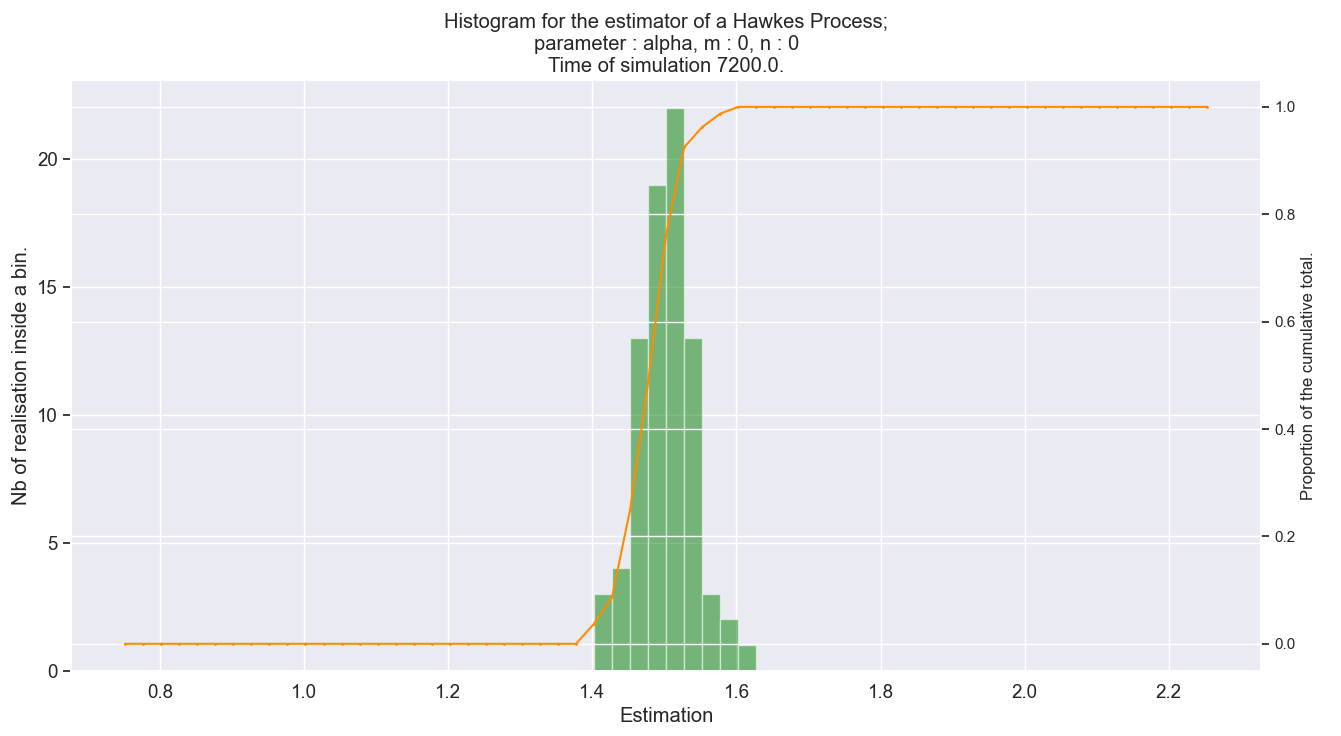
\includegraphics[width = 0.75 \textwidth]{../imag/chap2/hist_1.png}
\caption{Histogram for the estimations of a Hawkes Process. The process generates roughly 3000 jumps.}
\label{fig:hist_1_alpha}
\end{figure}


\begin{figure}
\centering
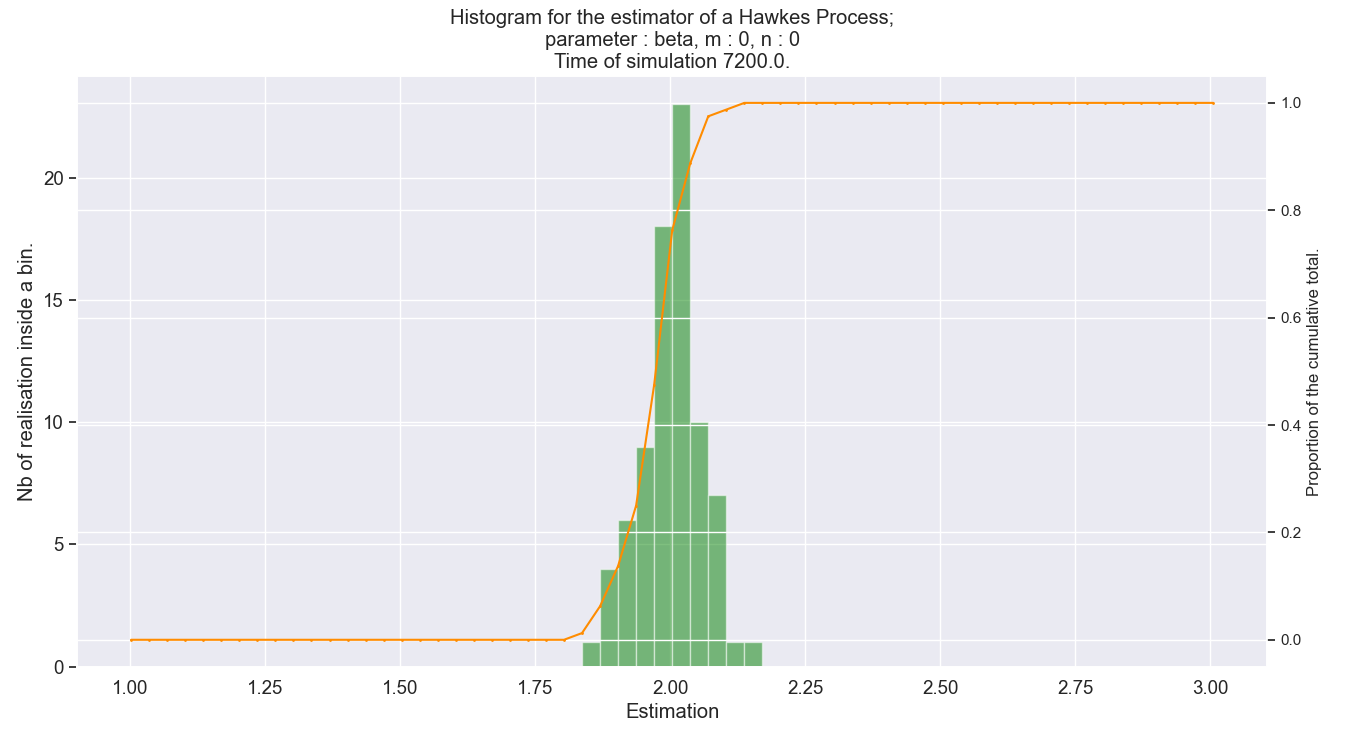
\includegraphics[width = 0.75 \textwidth]{../imag/chap2/hist_2.png}
\caption{Histogram for the estimations of a Hawkes Process. The process generates roughly 3000 jumps.}
\label{fig:hist_1_beta}
\end{figure}


\begin{figure}
\centering
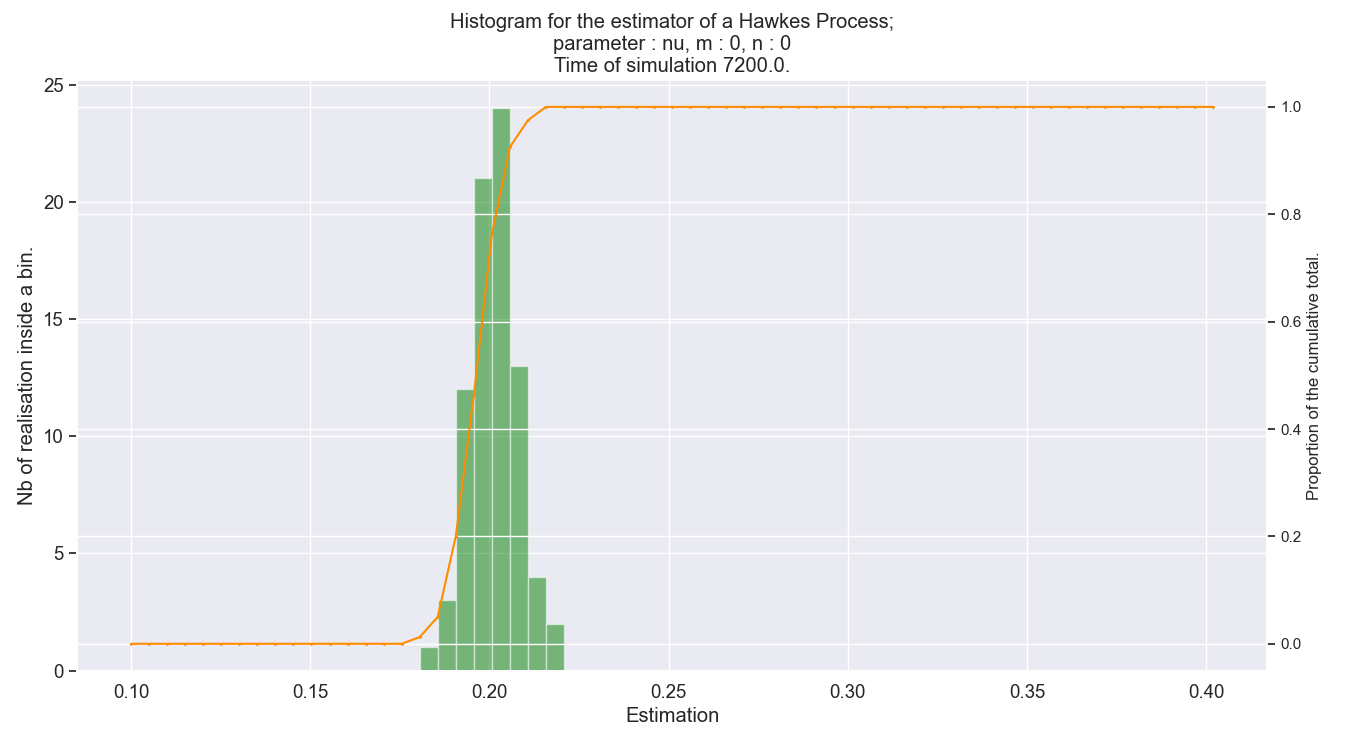
\includegraphics[width = 0.75 \textwidth]{../imag/chap2/hist_3.png}
\caption{Histogram for the estimations of a Hawkes Process. The process generates roughly 3000 jumps.}
\label{fig:hist_1_nu}
\end{figure}


\subsection{Asymptotic Consistency}

We can also run the program in order to compute the asymptotic MSE, with the number of observed jumps increasing with times. We plot the normalised MSE (mean MSE over the batch) score with respect to the number of observed jumps, for batches of 80 simulations. With the libray, we also plot the histogram of the batch with the highest simulated time. We observe the evolution of the MSE on figure \ref{fig:MSE_1}.





\begin{figure}
\centering
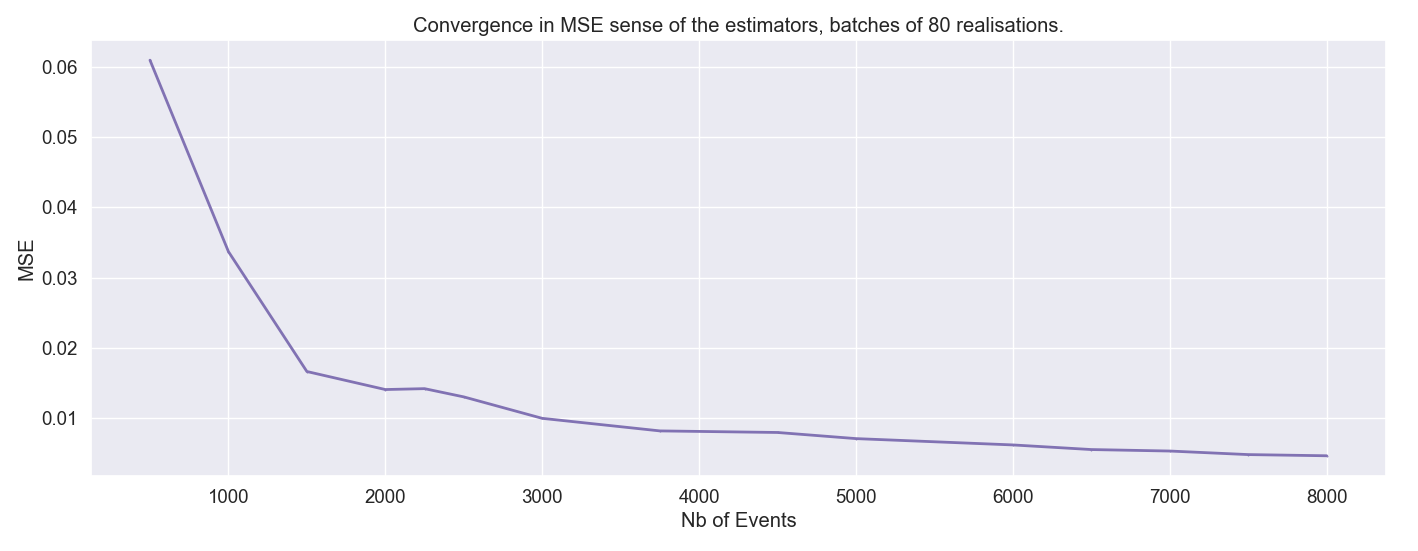
\includegraphics[width = 0.99 \textwidth]{../imag/chap2/MSE_score.png}
\caption{Evolution of the MSE for the estimations of a Hawkes Process.}
\label{fig:MSE_1}
\end{figure}

\subsection{Gradient and Hessian's structure}
The derivatives are obviously at least $\mathcal C^2$. Thus, by using Schwartz theorem, the gradient exists, so does the hessian and the latter is symmetric. This is pretty important because it allows to reduce the number of required computations by almost $2$. In other words, by keeping the notation from further-on, we can use, 

$$\forall i,j \in  \llbracket 1, M \rrbracket ^ 2,  H_{i,j} = H_{j,i}^T, \quad \text{and  } \forall i \in  \llbracket 1, M \rrbracket, H_{i,i} \text{ is symmetric.} $$


Hereinafter we draw a proposition for the structure of the gradient and the hessian, coined respectively by $D$ and $H$, for a M-variate Hawkes process:

\begin{equation}
D = \left ( 
\frac{\partial } {\partial \nu_1}, \cdots, \frac{\partial } {\partial \nu_M}
, 
\frac{\partial } {\partial \alpha_{1,1}},  \cdots, 
\frac{\partial } {\partial \alpha_{1,M}}, 
\frac{\partial } {\partial  \alpha_{2,1}}, \cdots, 
\frac{\partial } {\partial  \alpha_{M,M}}, 
\frac{\partial } {\partial  \beta_{1,1}}, \cdots, 
\frac{\partial } {\partial  \beta_{1,M}}, 
\frac{\partial } {\partial \beta_{2,1}}, \cdots, 
\frac{\partial } {\partial  \beta_{M,M}}  \right ) 
\end{equation}

By separating the Hessian into 9 pieces:

\begin{equation}
H = 
\begin{pmatrix}
H_{1,1} & H_{1,2}    & H_{1,3}  \\
H_{2,1}   &  H_{2,2}   & H_{2,3}\\
H_{3,1}      & H_{3,2}       &  H_{3,3}
\end{pmatrix}
\end{equation}

Where each individual piece reads, and we highlighted the groups of the same derivatives in respective colors:
\begin{equation}
H_{1,1} = 
\begin{pmatrix}
\textcolor{blue}{\frac{\partial^2 } {\partial \nu_1 \partial \nu_1 }} & 0       & \cdots & 0 & 0       \\
0      & \textcolor{blue}{\frac{\partial^2 } {\partial \nu_2 \partial \nu_2 }}
  & \cdots      &  0 & 0       \\
0      & 0       &  \textcolor{blue}{\frac{\partial^2 } {\partial \nu_3 \partial \nu_3 }}
     & \cdots & \vdots  \\
\vdots & \vdots  & \vdots & \textcolor{blue}{\ddots} & 0       \\
0      & 0       & \cdots & 0      & \textcolor{blue}{\frac{\partial^2 } {\partial \nu_M \partial \nu_M }}
\end{pmatrix}
\end{equation}

$$ H_{2,2} = $$
\begin{equation}
\begin{pmatrix}
\textcolor{blue}{\frac{\partial^2 } {\partial \alpha_{1,1} \partial \alpha_{1,1} }          } 
&
 \textcolor{red}{\cdots }
& 
 \textcolor{red}{\frac{\partial^2 }{\partial \alpha_{1,1} \partial \alpha_{1,M} } } 
&
0 & \cdots & 0 & 
\cdots & 0 & 
 \cdots 
&
  0      
\\%1
\textcolor{red}{\vdots  }     &  \textcolor{blue}{\ddots }  & \textcolor{red}{\vdots} & \vdots & \cdots & \vdots   & \cdots & \vdots & \cdots & \vdots  
\\%2
\textcolor{red}{\frac{\partial^2 }{\partial \alpha_{1,M} \partial \alpha_{1,1} } } & 
\textcolor{red}{\cdots}  & 
\textcolor{blue}{\frac{\partial^2 }{\partial \alpha_{1,M} \partial \alpha_{1,M} }} & 
 0 & \cdots & 0 & \cdots   & \vdots & \cdots & \vdots     
\\%3
0  & 
\cdots & 0 & 
\textcolor{blue}{\frac{\partial^2 } {\partial \alpha_{2,1} \partial \alpha_{2,1} }} &
\textcolor{red}{\cdots} & 
\textcolor{red}{\frac{\partial^2 } {\partial \alpha_{2,1} \partial \alpha_{2,M} }}      & 
\cdots & \vdots & \cdots & \vdots
\\%4
0  & 
\cdots & 0 & 
\textcolor{red}{\vdots} &
\textcolor{blue}{\ddots }& 
\textcolor{red}{\vdots } & 
\cdots & \vdots & \cdots & \vdots
\\ %5
0 &
\cdots & 0 & 
\textcolor{red}{\frac{\partial^2 } {\partial \alpha_{2,M} \partial \alpha_{2,1} }} &
\textcolor{red}{\cdots} & 
\textcolor{blue}{\frac{\partial^2 } {\partial \alpha_{2,M} \partial \alpha_{2,M} }}      & 
\cdots & \vdots & \cdots & \vdots
\\ %6
\vdots    &
\vdots & 
\vdots      & 
\vdots & \vdots & \vdots & \ddots &
\vdots & 
\vdots & 
\vdots
\\ %7
0      & 
\cdots & 
0      & 
0 & 
\cdots & 
0  & \cdots &
\textcolor{red}{\frac{\partial^2 } {\partial \alpha_{M,M-1} \partial \alpha_{M,M} }} &
\textcolor{red}{\cdots} & 
\textcolor{blue}{\frac{\partial^2 } {\partial \alpha_{M,M} \partial \alpha_{M,M} }}
\end{pmatrix}
\end{equation}




$$ H_{3,3} = $$
\begin{equation}
\begin{pmatrix}
\textcolor{blue}{\frac{\partial^2 } {\partial \beta_{1,1} \partial \beta_{1,1} }          } 
&
 \textcolor{red}{\cdots }
& 
 \textcolor{red}{\frac{\partial^2 }{\partial \beta_{1,1} \partial \beta_{1,M} } } 
&
0 & \cdots & 0 & 
\cdots & 0 & 
 \cdots 
&
  0      
\\%1
\textcolor{red}{\vdots  }     &  \textcolor{blue}{\ddots }  & \textcolor{red}{\vdots} & \vdots & \cdots & \vdots   & \cdots & \vdots & \cdots & \vdots  
\\%2
\textcolor{red}{\frac{\partial^2 }{\partial \beta_{1,M} \partial \beta_{1,1} } } & 
\textcolor{red}{\cdots}  & 
\textcolor{blue}{\frac{\partial^2 }{\partial \beta_{1,M} \partial \beta_{1,M} }} & 
 0 & \cdots & 0 & \cdots   & \vdots & \cdots & \vdots     
\\%3
0  & 
\cdots & 0 & 
\textcolor{blue}{\frac{\partial^2 } {\partial \beta_{2,1} \partial \beta_{2,1} }} &
\textcolor{red}{\cdots} & 
\textcolor{red}{\frac{\partial^2 } {\partial \beta_{2,1} \partial \beta_{2,M} }}      & 
\cdots & \vdots & \cdots & \vdots
\\%4
0  & 
\cdots & 0 & 
\textcolor{red}{\vdots} &
\textcolor{blue}{\ddots }& 
\textcolor{red}{\vdots } & 
\cdots & \vdots & \cdots & \vdots
\\ %5
0 &
\cdots & 0 & 
\textcolor{red}{\frac{\partial^2 } {\partial \beta_{2,M} \partial \beta_{2,1} }} &
\textcolor{red}{\cdots} & 
\textcolor{blue}{\frac{\partial^2 } {\partial \beta_{2,M} \partial \beta_{2,M} }}      & 
\cdots & \vdots & \cdots & \vdots
\\ %6
\vdots    &
\vdots & 
\vdots      & 
\vdots & \vdots & \vdots & \ddots &
\vdots & 
\vdots & 
\vdots
\\ %7
0      & 
\cdots & 
0      & 
0 & 
\cdots & 
0  & \cdots &
\textcolor{red}{\frac{\partial^2 } {\partial \beta_{M,M-1} \partial \beta_{M,M} }} &
\textcolor{red}{\cdots} & 
\textcolor{blue}{\frac{\partial^2 } {\partial \beta_{M,M} \partial \beta_{M,M} }}
\end{pmatrix}
\end{equation}


$$ H_{2,3} = $$
\begin{equation}
\begin{pmatrix}
\textcolor{blue}{\frac{\partial^2 } {\partial \alpha_{1,1} \partial \beta_{1,1} }          } 
&
 \textcolor{red}{\cdots }
& 
 \textcolor{red}{\frac{\partial^2 }{\partial \alpha_{1,1} \partial \beta_{1,M} } } 
&
0 & \cdots & 0 & 
\cdots & 0 & 
 \cdots 
&
  0      
\\%1
\textcolor{red}{\vdots  }     &  \textcolor{blue}{\ddots }  & \textcolor{red}{\vdots} & \vdots & \cdots & \vdots   & \cdots & \vdots & \cdots & \vdots  
\\%2
\textcolor{red}{\frac{\partial^2 }{\partial \alpha_{1,M} \partial \beta_{1,1} } } & 
\textcolor{red}{\cdots}  & 
\textcolor{blue}{\frac{\partial^2 }{\partial \alpha_{1,M} \partial \beta_{1,M} }} & 
 0 & \cdots & 0 & \cdots   & \vdots & \cdots & \vdots     
\\%3
0  & 
\cdots & 0 & 
\textcolor{blue}{\frac{\partial^2 } {\partial \alpha_{2,1} \partial \beta_{2,1} }} &
\textcolor{red}{\cdots} & 
\textcolor{red}{\frac{\partial^2 } {\partial \alpha_{2,1} \partial \beta_{2,M} }}      & 
\cdots & \vdots & \cdots & \vdots
\\%4
0  & 
\cdots & 0 & 
\textcolor{red}{\vdots} &
\textcolor{blue}{\ddots }& 
\textcolor{red}{\vdots } & 
\cdots & \vdots & \cdots & \vdots
\\ %5
0 &
\cdots & 0 & 
\textcolor{red}{\frac{\partial^2 } {\partial \alpha_{2,M} \partial \beta_{2,1} }} &
\textcolor{red}{\cdots} & 
\textcolor{blue}{\frac{\partial^2 } {\partial \alpha_{2,M} \partial \beta_{2,M} }}      & 
\cdots & \vdots & \cdots & \vdots
\\ %6
\vdots    &
\vdots & 
\vdots      & 
\vdots & \vdots & \vdots & \ddots &
\vdots & 
\vdots & 
\vdots
\\ %7
0      & 
\cdots & 
0      & 
0 & 
\cdots & 
0  & \cdots &
\textcolor{red}{\frac{\partial^2 } {\partial \alpha_{M,M-1} \partial \beta_{M,M} }} &
\textcolor{red}{\cdots} & 
\textcolor{blue}{\frac{\partial^2 } {\partial \alpha_{M,M} \partial \beta_{M,M} }}
\end{pmatrix}
\end{equation}


$$H_{1,2} =  $$
\begin{equation}
\begin{pmatrix}
\textcolor{blue}{\frac{\partial^2 } {\partial \nu_1 \partial \alpha_{1,1} }}
&
 \textcolor{blue}{\cdots }
& 
 \textcolor{blue}{\frac{\partial^2 }{\partial \nu_1 \partial \alpha_{1,M} } } 
&
0 & \cdots & 0  & \cdots & 0 & \cdots & 0
\\%1
0       &  \cdots   & 0 &  
\textcolor{blue}{\frac{\partial^2 }{\partial \nu_2 \partial \alpha_{2,1} }}  & 
\textcolor{blue}{\cdots} &  
\textcolor{blue}{\frac{\partial^2 }{\partial \nu_2 \partial \alpha_{2,M} }} & \cdots & 0 & \cdots & 0
\\%2
\vdots & \vdots & \vdots & \vdots & \vdots & \vdots  & \ddots & \vdots & \vdots & \vdots
\\%3
0  & \cdots & 0 & 0 & \cdots & 0 & \cdots & 
\textcolor{blue}{\frac{\partial^2 } {\partial \nu_M \partial \alpha_{M,1} }} &
\textcolor{blue}{\cdots} & 
\textcolor{blue}{\frac{\partial^2 } {\partial \nu_M \partial \alpha_{M,M} } }
\end{pmatrix}     
\end{equation}

$$H_{1,3} = $$
\begin{equation} 
\begin{pmatrix}
\textcolor{blue}{\frac{\partial^2 } {\partial \nu_1 \partial \beta_{1,1} }}
&
 \textcolor{blue}{\cdots }
& 
 \textcolor{blue}{\frac{\partial^2 }{\partial \nu_1 \partial \beta_{1,M} } } 
&
0 & \cdots & 0  & \cdots & 0 & \cdots & 0
\\%1
0       &  \cdots   & 0 &  
\textcolor{blue}{\frac{\partial^2 }{\partial \nu_2 \partial \beta_{2,1} }}  & 
\textcolor{blue}{\cdots} &  
\textcolor{blue}{\frac{\partial^2 }{\partial \nu_2 \partial \beta_{2,M} }} & \cdots & 0 & \cdots & 0
\\%2
\vdots & \vdots & \vdots & \vdots & \vdots & \vdots  & \ddots & \vdots & \vdots & \vdots
\\%3
0  & \cdots & 0 & 0 & \cdots & 0 & \cdots & 
\textcolor{blue}{\frac{\partial^2 } {\partial \nu_M \partial \beta_{M,1} }} &
\textcolor{blue}{\cdots} & 
\textcolor{blue}{\frac{\partial^2 } {\partial \nu_M \partial \beta_{M,M} } }
\end{pmatrix}     
\end{equation}


\subsection{Implementation Difficulties in Python}

\begin{itemize}
\item The first obvious difficulty has been to write down the formulas into code without mistake. The formulas are heavy and very prone to errors.
\item In particular, creating the Hessian was a riddle. We haven't found a clever way to write it properly. The author's idea was that we only need to create the upper part of the Hessian, and that there are two types of groups of derivatives: the square and the rectangles, as appearing in the previous subsection.
\item As mentioned, the computational bottleneck makes the algorithms slow. For that reason, the rest of the program has to be optimized in order to compensate that lack of performances. In particular, Python is a slow language. We heavily rely on numpy, a library with which all the numerical computations are made in C.
\item One shall also introduce some burn-in period before the actual useful part of the simulation of the process; cf. subsection \ref{subsection:burn}.
\item Certain sets of parameters lead to unprecise results. In particular, boundarie cases (as $\alpha = \beta$) are problematic, as well as sets of parameters with not enough events occuring during the simulation. The observed interval should be adapted to the parameters. In other words, it is less interesting to talk about the interval [0,T] for simulations than rather the number of events occuring on that interval.
\end{itemize}

With regards to computational optimization, we mainly made usage of numpy for computations involving long vectors. In particular, using the built-in function for exponential makes running much faster. 

We also used this trick for computing $R,R',R''$. One can actually compute R' and R'' at the same time in order to spare some redundant computations. Finally, by using a matrix notation (through the function "np.subtract.outer(,)"), numpy can compute those quantities for all the dimensions (in the multi-dimensional case) at once. The code would look like this:

\begin{verbatim}
def compute_R_dashes(m, n, T_t, BETA):
    matrix_diff = np.subtract.outer(np.array(T_t[m]), np.array(T_t[n]))
    matrix_diff[matrix_diff < 0] = 0
    # faster than
    # matrix_diff = np.maximum(,0)

    dashes = matrix_diff * np.exp(-BETA[m, n] * matrix_diff)
    dash_dashes = dashes * matrix_diff
    # np.power is not efficient for scalars, but good looking.
    previous_Rs_dash[(m, n)] = list(dashes.sum(axis=1))

    previous_Rs_dash_dash[(m, n)] = list(dash_dashes.sum(axis=1))
\end{verbatim}

Some other hidden tricks have also been discovered by the author, like using binary operations instead of using logical notations, or list comprehension.

Last but not least, we used memoization (and in our case scenario using a decorator is possible) for $R,R',R''$. Memoisation is a programming technique which is used to speed up computations\footnote{It was derived from the Latin word memorandum which means “to be remembered”}. As the name suggests, it is based on memorizing the results of expensive function calls. Whenever the function is called again with the same parameters, the results does not have to be computed again and it avoids unnecessary calculations. With its recursive form, $R$ is then computed extremely quickly in linear time. Memoization in Python can be implemented with the help of a class-decorator, that one can dissect in the author's personal libraries section \ref{personal_lib}. 




\section{Numerical Results}



\subsection{Histogram}
The first thing to do is to run the simulation and the estimation for a given Hawkes Process. We chose a Hawkes process with parameters: $\alpha = 1.5, \beta = 2, \nu = 0.2$. We get the following histograms for the results, when we simulate the process over 7200 units of time (the algorithm observes roughly 3000 events) for a batch of 80 simulations. This leads to figures \ref{fig:hist_1_alpha}, \ref{fig:hist_1_beta}, \ref{fig:hist_1_nu}.

\begin{figure}
\centering
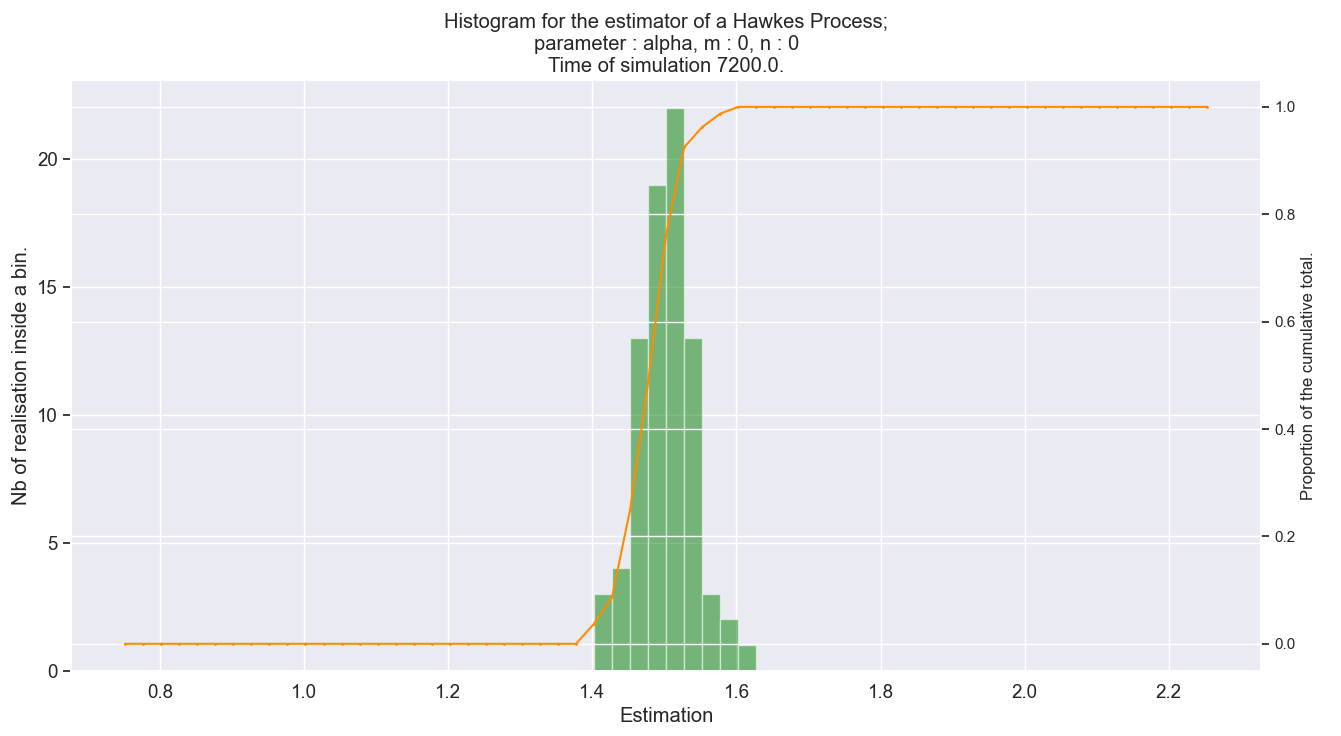
\includegraphics[width = 0.75 \textwidth]{../imag/chap2/hist_1.png}
\caption{Histogram for the estimations of a Hawkes Process. The process generates roughly 3000 jumps.}
\label{fig:hist_1_alpha}
\end{figure}


\begin{figure}
\centering
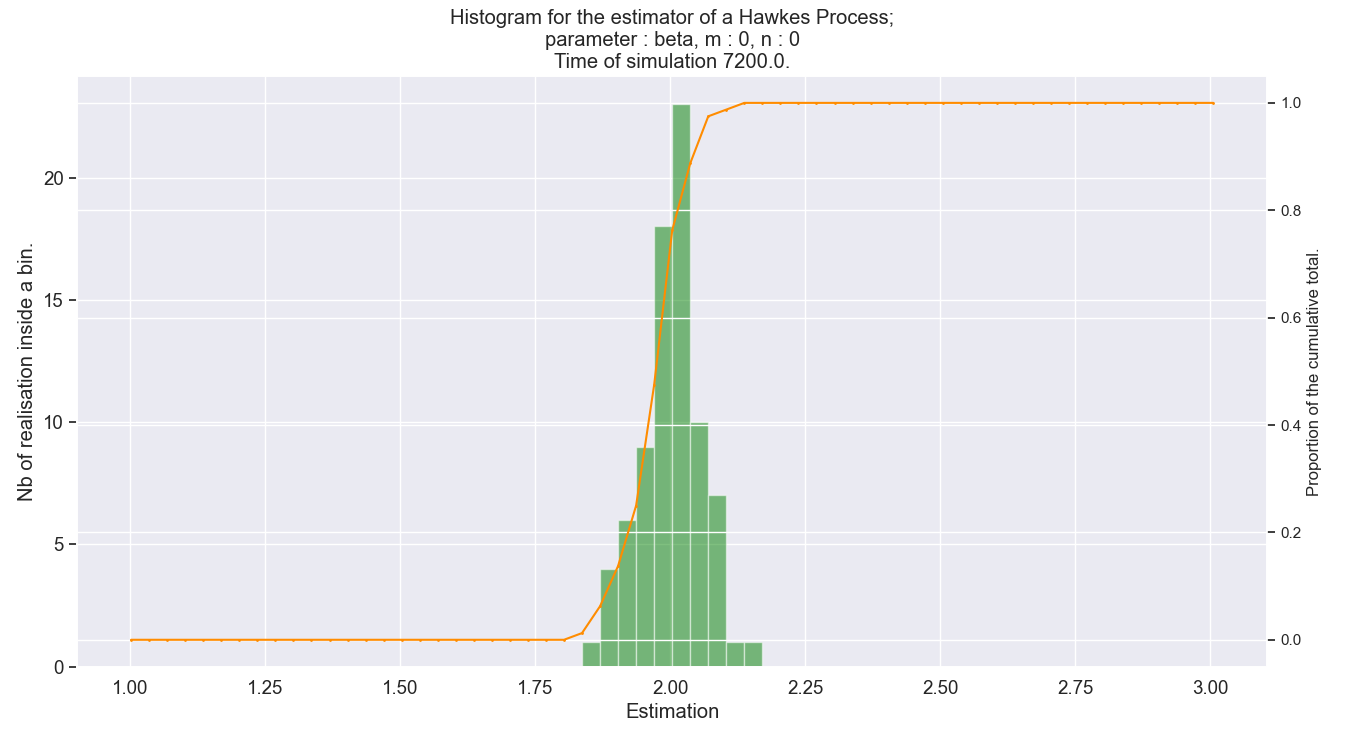
\includegraphics[width = 0.75 \textwidth]{../imag/chap2/hist_2.png}
\caption{Histogram for the estimations of a Hawkes Process. The process generates roughly 3000 jumps.}
\label{fig:hist_1_beta}
\end{figure}


\begin{figure}
\centering
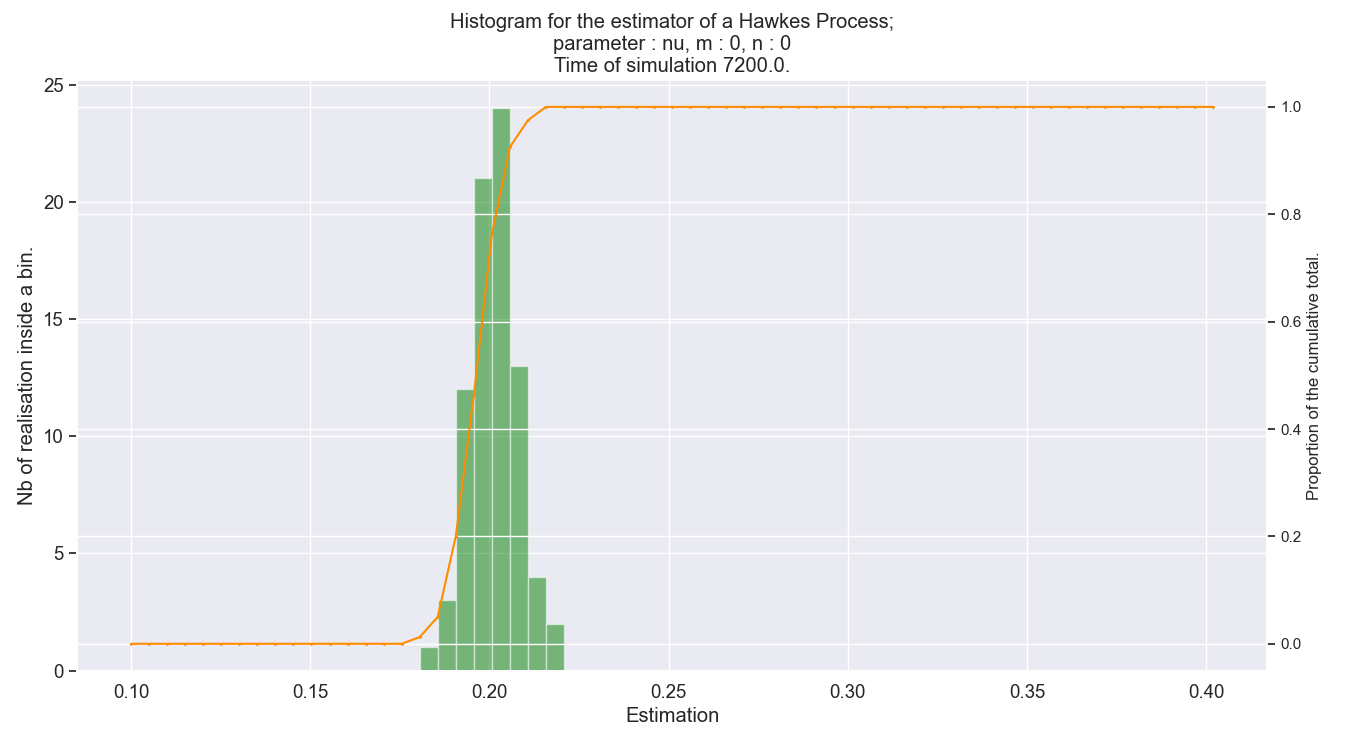
\includegraphics[width = 0.75 \textwidth]{../imag/chap2/hist_3.png}
\caption{Histogram for the estimations of a Hawkes Process. The process generates roughly 3000 jumps.}
\label{fig:hist_1_nu}
\end{figure}


\subsection{Asymptotic Consistency}

We can also run the program in order to compute the asymptotic MSE, with the number of observed jumps increasing with times. We plot the normalised MSE (mean MSE over the batch) score with respect to the number of observed jumps, for batches of 80 simulations. With the libray, we also plot the histogram of the batch with the highest simulated time. We observe the evolution of the MSE on figure \ref{fig:MSE_1}.





\begin{figure}
\centering
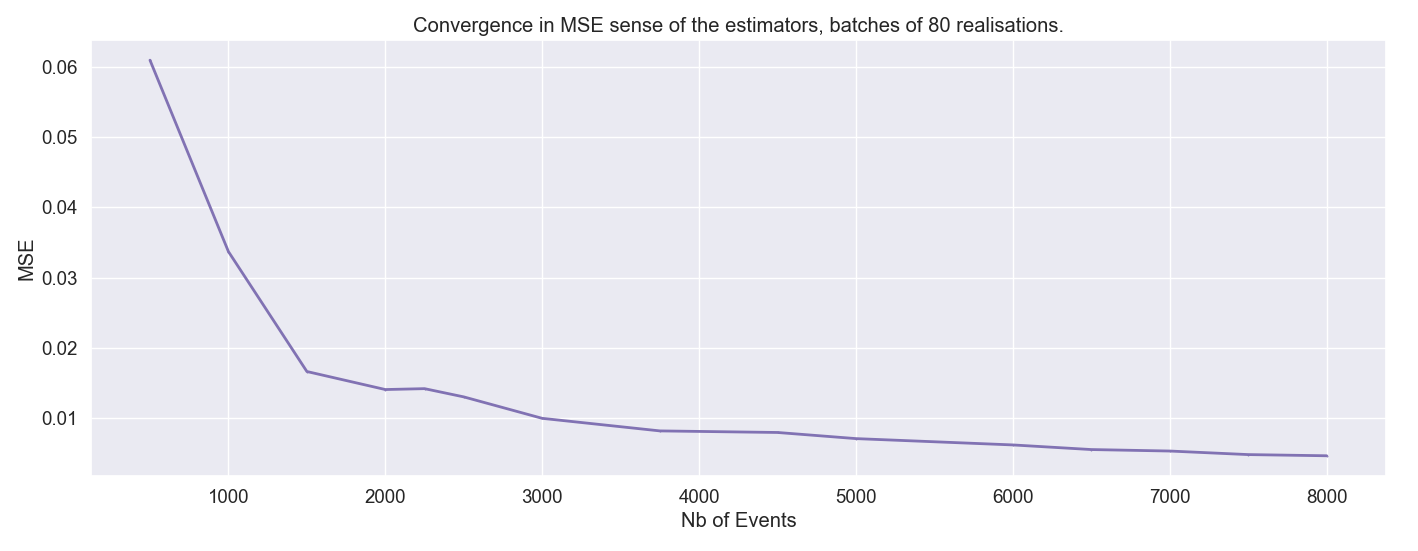
\includegraphics[width = 0.99 \textwidth]{../imag/chap2/MSE_score.png}
\caption{Evolution of the MSE for the estimations of a Hawkes Process.}
\label{fig:MSE_1}
\end{figure}





\chapter{Estimation: Advanced Glance on the Question}
\section{Weighted MLE}
\subsection{Theory of Weighting}
Following the computations from \cite{Ozaki} and \cite{Likelihood_Hawkes} about the likelihood function of a Hawkes process, we get a formula for a multidimensional ($ M \in \mathbb N^*$) Hawkes process, defined on the interval $[0,T]$, with jumps at times: $ \forall m \leq M: 0 < t_{1}^m \cdots < t_{n_m}^m \leq T $.

We recall that $ \Tau^m $ is referring to the list history, including the jumps' time $( t_{1}^m, \cdots , t_{n_m}^m ) $, and the marks; $\Theta$ represents the set of parameters of the process. Finally, the superscript visible on $L^m$ is mentioned in order to avoid confusion between each likelihood function of each marginal process (with respect to the multi-dimensional Hawkes process). The marginal log-likelihood reads (cf. eq. (\ref{eq:intensity_lambda})):


\begin{equation}
\ln L^m( \Theta \mid \Tau ) = - \int_0^T \lambda^{m} ( s \mid \Theta , \Tau ) ds + \int_0^T \ln \lambda^{m}( s \mid \Theta , \Tau ) d N_s^m \label{eq:log_likelihood}
\end{equation}



In section II from \cite{weighted_likelihood}, and by coining the weight function $w$\footnote{also called in the following kernel. We will introduce a difference of realm between the two in the next section in footnote \ref{section:diff_kernel_weights}. Since the difference is quite subtle, we use weights, kernel and window interchangeably.}, they define the weighted estimating equation as:

\begin{equation}
\ln W L ( \Theta \mid \{ X_1, \cdots, X_n \} ) = \sum_1^n  w(X_i) \ln f( X_i \mid \Theta ) 
\end{equation}

We emphasize on the notation WL to highlight the spirit of the weighted likelihood estimation problem, which is different from the classic likelihood estimation problem.


In our case scenario, we add up a time dependence upon the kernel, and replace the $\sequence{X_i}$'s by $\sequence{t_i}$'s.


Remember that we had from eq. (\ref{eq:ln_multi}):
 
\begin{equation}
\ln L( \Theta \mid \Tau ) = \sum_1^M \ln L^m( \Theta \mid \Tau )
\end{equation}

And this is also true for the weighted likelihood. Hence, focusing on our marginal weighted likelihood, the estimating equation reduces to:



\begin{align}
\ln W L^m( \Theta \mid \Tau ) &= - \int_0^T w(s) \lambda^{m} ( s \mid \Theta , \Tau ) ds + \int_0^T w(s) \ln \lambda^{m} ( s \mid \Theta , \Tau ) d N_s^m  
\label{eq:weighted_log_likelihood} \\
&=  - \int_0^T w(s) \lambda^{m} ( s \mid \Theta , \Tau )  ds +  \sum^{n_m}_i  w(t_i) \ln \lambda^{m} ( t_i \mid \Theta , \Tau )  \label{eq:weighted_log_likelihood2} 
\end{align}

Notice how if all the weights are equal to unity, then the resulting estimator is the usual maximum likelihood estimator, i.e. if $w \equiv 1$, then eq. (\ref{eq:weighted_log_likelihood}) becomes eq. (\ref{eq:log_likelihood}). We wrote down explicitly eq. (\ref{eq:weighted_log_likelihood2}) in order to emphasize how the kernel function becomes random through the jumps' time $t_i$. 

Weighting should be a way to rescale the information at our disposal. For that reason, we restrict the set of considered kernels to be of norm $T$:

$$\Omega_w := \{ w \colon \mathbb R \to \mathbb R, \text{ such that : } \norm{w}_{L^1 } = T \} $$

By this, we ensure that we conserve, using the physical expression, the energy of each integrand. Also, notice that for the non-weighted case, when $w \equiv 1$, its norm is equal to $T$. That's the reason why we fix the value of the norm of every kernel inside $\Omega_w$ to $T$. Also, we do not need any other restriction on the considered functions. However, one usually considers fixing as well the positivity of kernel and its first moments, for identifiability reasons. Those conditions ensure that the kernels are densities, an enjoyable feature when one estimates densities. 

\subsection{Advantage and Notation of WMLE}

The idea behind using weighted likelihood is that by using a non-constant weight function, solving for the maximum likelihood estimator given by eq. (\ref{eq:weighted_log_likelihood}) can potentially outperform the one given by eq. (\ref{eq:log_likelihood}). 

Let's think about the two extreme cases: 

\begin{enumerate}
\item a constant kernel considers all the jumps equally and hence, computes an estimator that is equal to the average of the whole simulation time $[0,T]$.
\item a kernel that considers only a small region will give a very precise estimate for that given region, but with much more variability over the time.
\end{enumerate}

This phenomenon is due to the well-known bias/variance trade-off.
\label{section:bias-variance_trade-off}

Essentially, we want to take advantage of the fact that a larger weight w(s) gives to observations in the infinitesimal region $ds$ more influence on the estimation process. This would allow us to estimate parameters that are time dependent by adding that dependence within kernels. Now the main question shall be which kernel should we chose. Recall what Silverman said in \cite{Silverman} at page 43:

\vspace{0.5cm}
\textit{It should never be forgotten that the appropriate choice of smoothing parameter will always be influenced by the purpose for which the density estimate is to be used. }
\vspace{0.5cm}


\label{section:kernel_weights_first_conversation}
In the rest of the chapter, we delve into the choice of such windows in order to optimize the performances of the WMLE. Our aim being to estimate parameters that are time dependent, we add that dependency to the WMLE through the kernel, which should be written consequently $w_t$. However, for clarity, it will be kept as $w$. We need to mention an important matter in order to avoid any confusion. Our weight function is evaluated at the points $\sequence{t_i}$ when the jumps of the Hawkes process occur. Also, the time dependence is introduced by centring the kernel around $t$ by a classic substitution: 

$$w(t_i) \to w(  t_i - t ) $$

For the same reasons as not underlying $t$ as a subscript, we are not going to write this change of variable inside $w$, in the exact same way we did so far. The times $t$ at which we want to estimate the parameters can't be coined as $\sequence{t_i}$ since it is already our notation for the jumps' time. Hence, we will write these times as $\sequencetime$.

In the following, we are going to delve into the theory of KDE, where it is common to use the letter $K$ instead of $w$. Also, the objective is slightly different. KDE's aim is to find the estimate of a function $f$ evaluated at the point $t$ by using kernels centred around $t_i$. For that reason, people are using kernels with the following substitution:

$$ K(t) \to K(t - t_i)$$

Hence, in order to avoid confusion, we keep for a few theoretical sections the notation $K$ for kernels, within which we write the substitution. Later, we do propose a definition in section \ref{section:equivalence_bi_rep} that splits the two objects into distinct concepts.


\subsection{WMLE Algorithm}
It could be possible to parametrize the MLE we are using. However, we are not changing at the essence, the algorithm from the previous chapter. 

The necessary adaptation one has to do is to multiply the contribution of each jump to the log-likelihood by the corresponding weight. This is a given, as long as the weights are $\alpha, \beta, \nu$-independent\footnote{Ensuring that the derivatives do not change, up to a multiplicative constant.}. 

The idea of mixing the dependency of the parameters inside the weights in order to improve performances is something that could be done. It would basically be parametrizing the MLE. If for instance we are estimating the parameter at $t_2$ with $t_1 < t_2$, an idea could be to use the already done estimation at $t_1$ for computing the estimation at $t_2$.





\section{Choice of the Window}

We mentioned our wish of estimating the parameters with some time-dependence. By inspiring ourselves from kernel density estimation (KDE) theory, we hope to be also able to estimate correctly the evolution of the parameters through time. The main difference between KDE and our task is that our estimate won't be a density function\footnote{Hence, the integral of the function does not have to yield $1$. However, notice that the condition set on our model ensures that all parameters are positive, thus, the functions are always positive}. 

In the following, we consider solely $1$-D kernels, which are weighting the maximum likelihood estimation\footnote{Kernels are by definition density functions usually coined in the literature by the symbol $K$. On the other hand, we are interested in weights $w$. For the following theoretical bit, we keep the notation from KDE since it is where the ideas come from. However, without loss of generality, one can scale kernels in order to get weights back. Thus, kernels are to weights what probability measures are to measures\label{section:diff_kernel_weights}.}. The latter leads to a parameter $\theta^* \in \Theta$, the MLE, which belongs to $\mathbb R^{m+2 m^2}$. We shall also underline on the variable the dependency on time $t$ with a subscript, which comes from the evaluation of the kernel at a precise time. If the variable $t$ was continuous, we would hence have a function $$\theta^*_t \colon \mathbb R  \to R^{m+2 m^2} $$

We would like to find the such best function, with respect to certain criteria, with respect to the choice of the kernel. For the theoretical part, we will look at a real-valued function $f$ without loss of generality. Indeed, defining an operator on $f$ is equivalent to define an operator on $\norm{\theta^*_t}$ where $\norm{\cdot}$ is any norm equipping $\mathbb R$.
\label{section:multi_to_uni}
\label{section:kernel_to_weights}













\subsection{Measure of Accuracy}
The class $ \Omega_w $ of functions is pretty big, and we would like to find the best kernels. For that reason, we first need to fix a metric in order to compare the scores of the different estimations. If one knows the true function estimated $f$, and calls the estimation $\hat{f}$, then one measure of accuracy is given by the mean square error, computed by: 

\begin{equation}
\MSE ( \hat{f}(u) ) \triangleq  \E [ ( \hat{f}(u) - f(u) )^2 ]
\end{equation}

whose global natural extension is given by the $L^1$ norm of the previous quantity, yielding the so-called mean integrated square error:

\begin{equation}
\MISE ( \hat{f}(u) ) \triangleq  \E [ \int ( \hat{f}(u) - f(u) )^2 du ]
\end{equation}

\begin{remarque}
One can rewrite, under mild condition of regularity:
\begin{align*}
\E [ \int ( \hat{f}(u) - f(u) )^2 du ] &= \int \E [( \hat{f}(u) - f(u) )^2 ] du \\
&= \int  \E[ (\hat{f}(u) ] - f(u) )^2 ] du + \int \Var( \hat{f}(u)) du 
\end{align*}
hence we came back to the classic bias-variance trade-off we already mentioned in section \ref{section:bias-variance_trade-off}.
\end{remarque}

Using the theory available in KDE, we are going to find the best kernels with respect to $\MISE$.

\section{Fixed Width Window}
\label{section:FWW}

A kernel is composed of two things: a basic canonical function shaping the kernel and the variables that adjust the values taken. A first thing to do would be to uncouple the two parameters.

\subsection{Optimal Kernel}

As exposed in \cite{Wand}, it is possible to derive the optimal kernel for KDE. In \cite{Wand}, the formula for asymptotical mean square error is given by their eq. (2.12). The issue there is that the scaling of $K$ is coupled with the bandwidth $h$. However, by a substitution inside $K$ of the form 
$$ K_{\delta} ( \cdot ) = \frac 1  {\delta } K \left ( \frac {\cdot } { \delta } \right ) $$
we get a factorization of the previous expression with separate dependency of the bandwidth and of the kernel. One has to simply choose $\delta$\footnote{Independent to $h$.} to be: $$ \delta_0 = \left ( \frac{ \int K(t)^2 dt }{ \left ( \int t^2 K(t) dt \right )^2 } \right ) ^{\frac 1 5} $$


\begin{theoreme}{Optimal kernel for KDE estimation choice}

\begin{equation}
\begin{array}{lcr}
\min_{ K  }  & C(K) := ( \mu_2 ^2 \cdot \norm{K}_{L^1}^4 )^{1/5}      &     \\
\text{subject to }   & K \geq 0 & \text{(positivity) } \\
& \norm{K}_{L^1} \triangleq  \int K = 1  & \text{(normalized)} \\
 & \mu_1 \triangleq  \int t K(t) dt = 0    & \text{(centred)                 } \\
& \mu_2 \triangleq  \int t^2 K(t) dt =: a         & \text{(finite second moment)   }           
\end{array}
\end{equation}

has the following class of kernels as a solution:

\begin{equation}
K^*_a(t) := \frac 3 4  \frac { 1 - \frac {t^2}{5 a^2} } {\sqrt{5} a } \11charac_{ \{ \abs t \leq \sqrt{5} a \} }
\end{equation} 

We usually refer to this class of kernel as Epanechnikov. It also is usual to fix $a=1$ and to rescale the kernel such that it is defined on $\abs t \leq 1 $, yielding:


\begin{equation}
K^*(t) := \frac 3 4 ( 1 - t^2 )  \11charac_{ \abs t \leq 1 }
\end{equation} 
\end{theoreme} 

The kernel that minimizes the target equation in the minimization problem is also the one which minimizes the $\MISE$. Actually, the quantity $C(K)$ is the kernel dependent part of the expression. 

Another popular scaled kernel, with almost equal performances is the biweight kernel defined as:

\begin{equation}
K_b(t) := \frac {15}{16} ( 1 - t^2 )^2  \11charac_{ \abs t \leq 1 }
\end{equation} 

\begin{remarque}
Note that the biweight kernel is of class $\mathcal C^{1}$ at $\{-1, 1\}$ while Epanechnikov isn't derivable at those points.
\end{remarque}











In order to compare the performances of different kernels, statisticians developed the concept of efficiency:

\begin{definition}[Efficiency of $K$ relative to $K^*$]
Efficiency represents the ratio of sample sizes necessary
to obtain the same accuracy when using $K^*$ as when using $K$. The efficiency is, thus, computed as:

$$ \left ( \frac{C(K^*)}{C(K)} \right ) ^{\frac 5 4 } $$
\end{definition}

Is shown page 31 in Table (2.1), in \cite{Wand}, Epanechnikov kernel has an efficiency of $1$, and the biweight has an efficiency of $0.994$. It is actually surprising how the windows aren't affecting efficiency in a very impactful manner.



\begin{remarque}
Four of the common kernels are actually derived with the same formula. They are all part of the same family:

$$ K(x,p) = \frac{(1-x^2)^p}{2^{2p+1} B(p+1,p+1) } \11charac_{\abs x < 1 }$$

where $B(\cdot, \cdot)$ is the beta function. Notice that $p=1$ corresponds to the Epanechnikov kernel, $p=2$ corresponds to the biweight kernel, $p=3$ matches with the often called triweight kernel and finally the limiting case of $p \to \infty$ corresponds to the standard normal density kernel. 
\end{remarque}


\begin{figure}
\centering
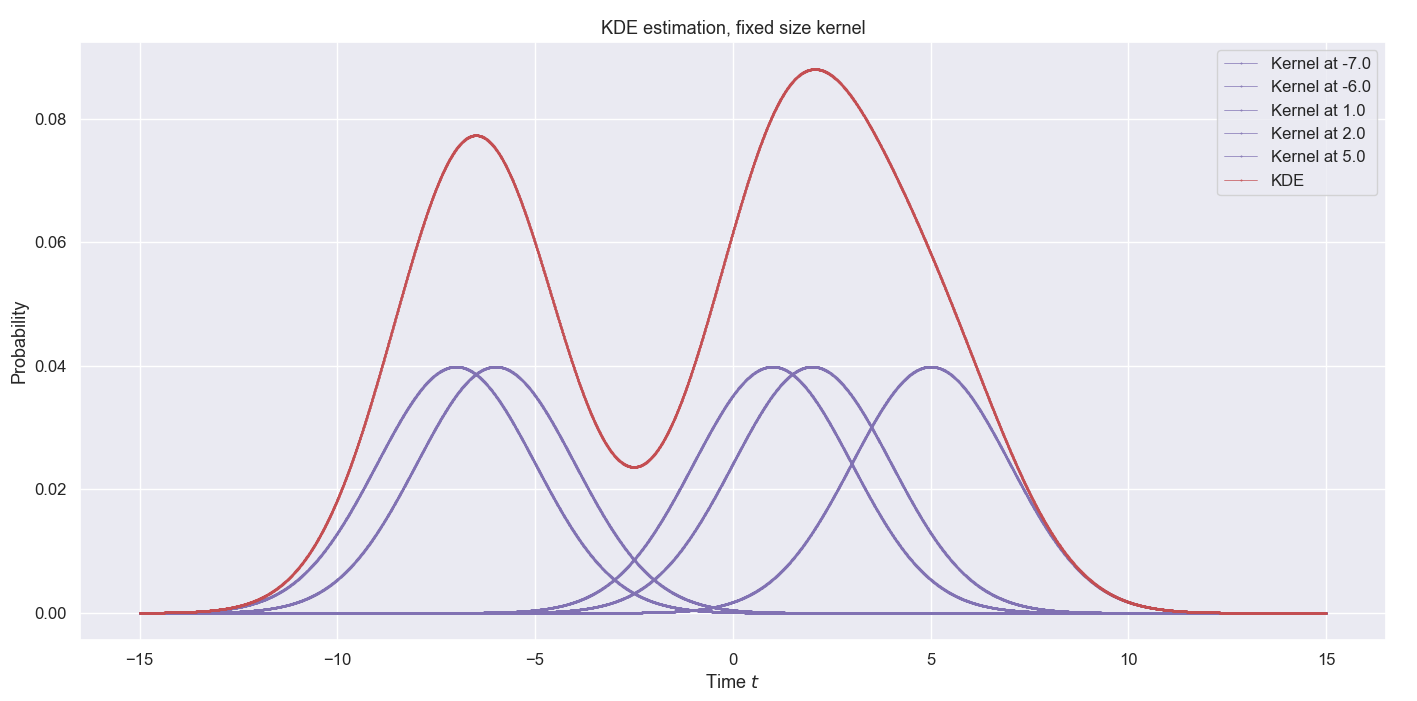
\includegraphics[width = 0.90 \textwidth]{../imag/chap3/FKDE.png}
\caption{Example of a fixed kernel density estimation, showing the impact of the single kernels.}
\label{fig:FKDE}
\end{figure}

\subsection{A Few Kernels That We Tried to Use}

By considering parameters that are constant through time, as displayed on fig. \ref{fig:evol_choice_basic}, we tested different kernels, for fixed width, essentially the one from fig. \ref{fig:kernels_list}. We got the results from fig. \ref{fig:basic_5_kernels_alpha}, \ref{fig:basic_5_kernels_beta}, \ref{fig:basic_5_kernels_nu}. We don't notice any noticeable change. Perhaps it would be interesting to compute the change in MSE depending on the kernel. This confirms our idea that the kernel doesn't impact the estimation too much.


\begin{figure}
\centering
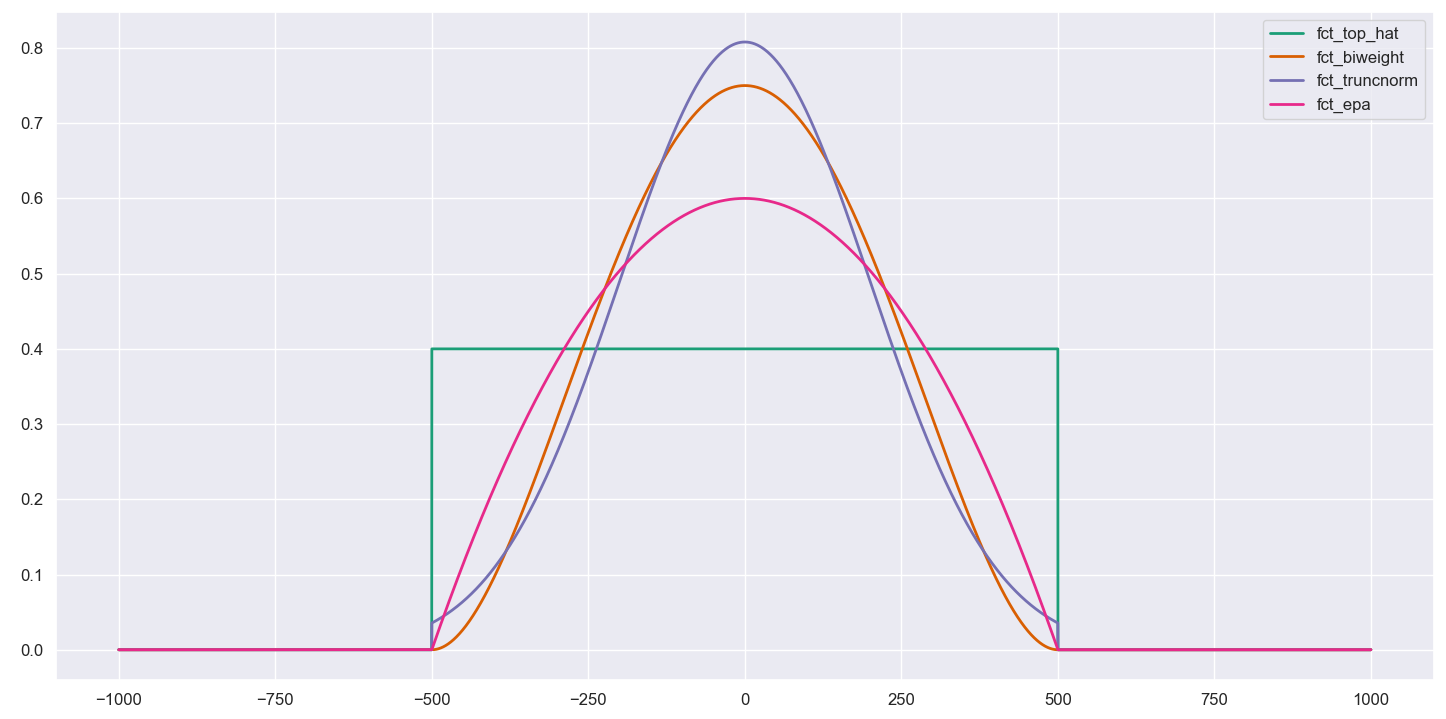
\includegraphics[width = 0.80 \textwidth]{../imag/chap3/the_kernels.png}
\caption{Superposition of the kernels shapes we mentioned.}
\label{fig:kernels_list}
\end{figure}


\begin{figure}
\centering
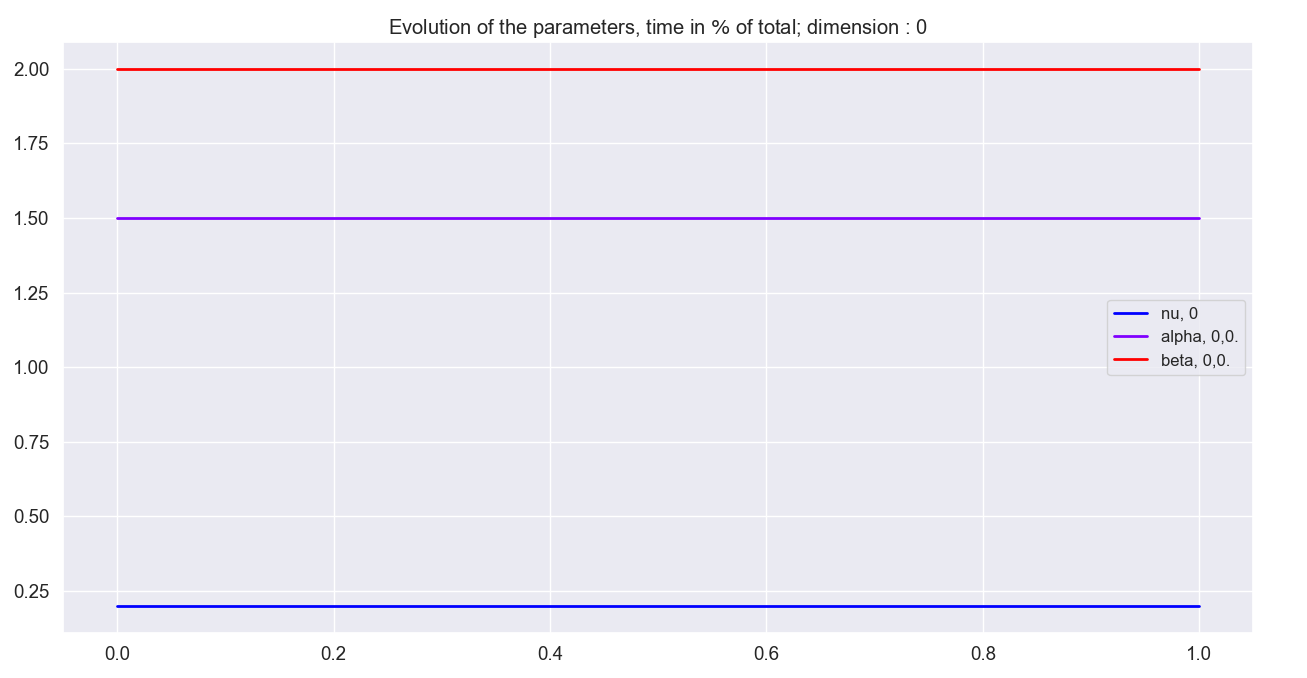
\includegraphics[width = 0.75 \textwidth]{../imag/chap3/compar_kernel/evol_param.png}
\caption{Parameters for fig. \ref{fig:basic_5_kernels_alpha}, \ref{fig:basic_5_kernels_beta}, \ref{fig:basic_5_kernels_nu}, and for next section: fig. \ref{fig:basic_3_kernels_alpha}, \ref{fig:basic_3_kernels_beta}, \ref{fig:basic_3_kernels_nu}. }
\label{fig:evol_choice_basic}
\end{figure}


\begin{figure}
\centering
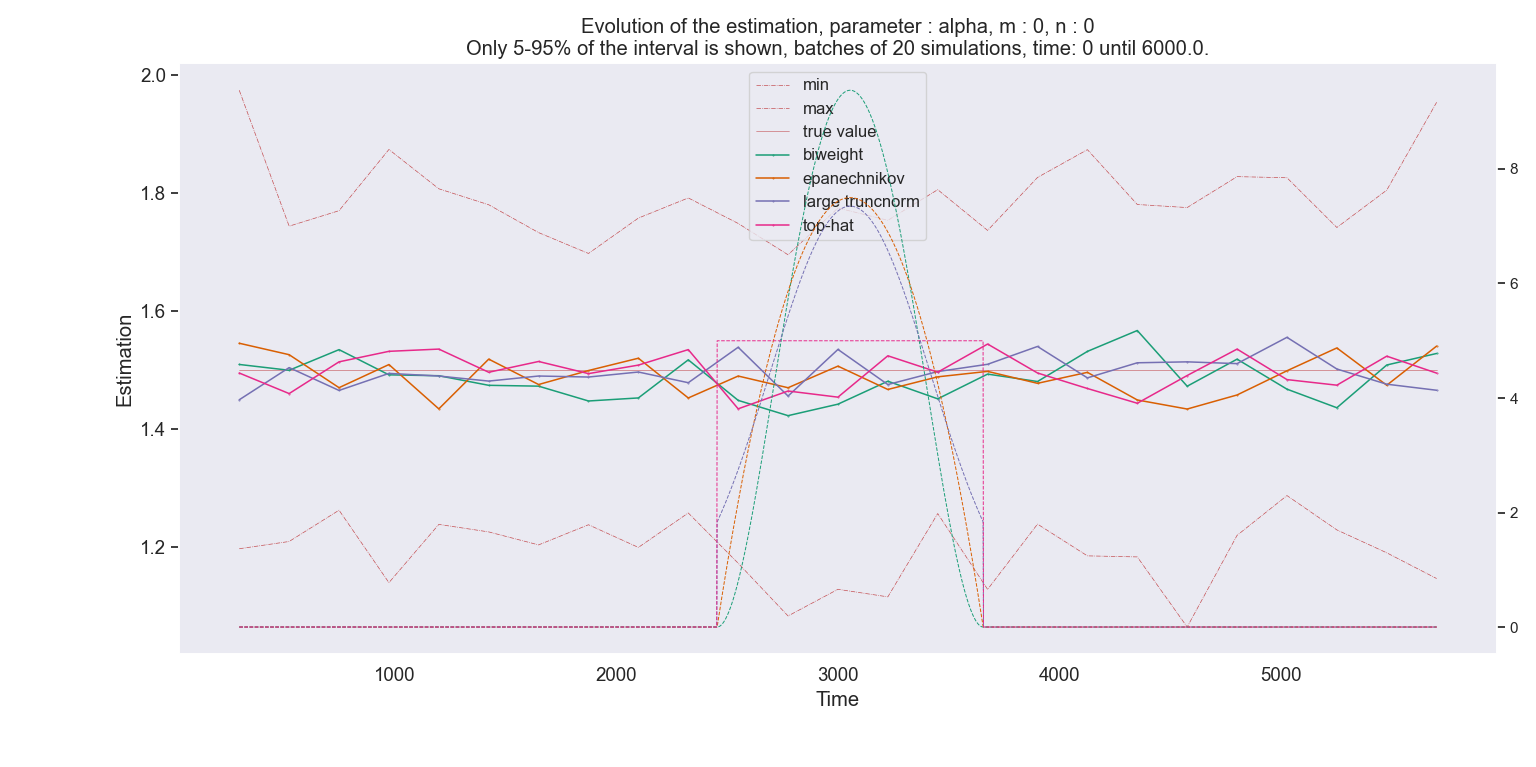
\includegraphics[width = 0.90 \textwidth]{../imag/chap3/compar_kernel/alpha.png}
\caption{Fixed kernel density estimation, showing the impact of the type of kernels. Plot of alpha.}
\label{fig:basic_5_kernels_alpha}
\end{figure}

\begin{figure}
\centering
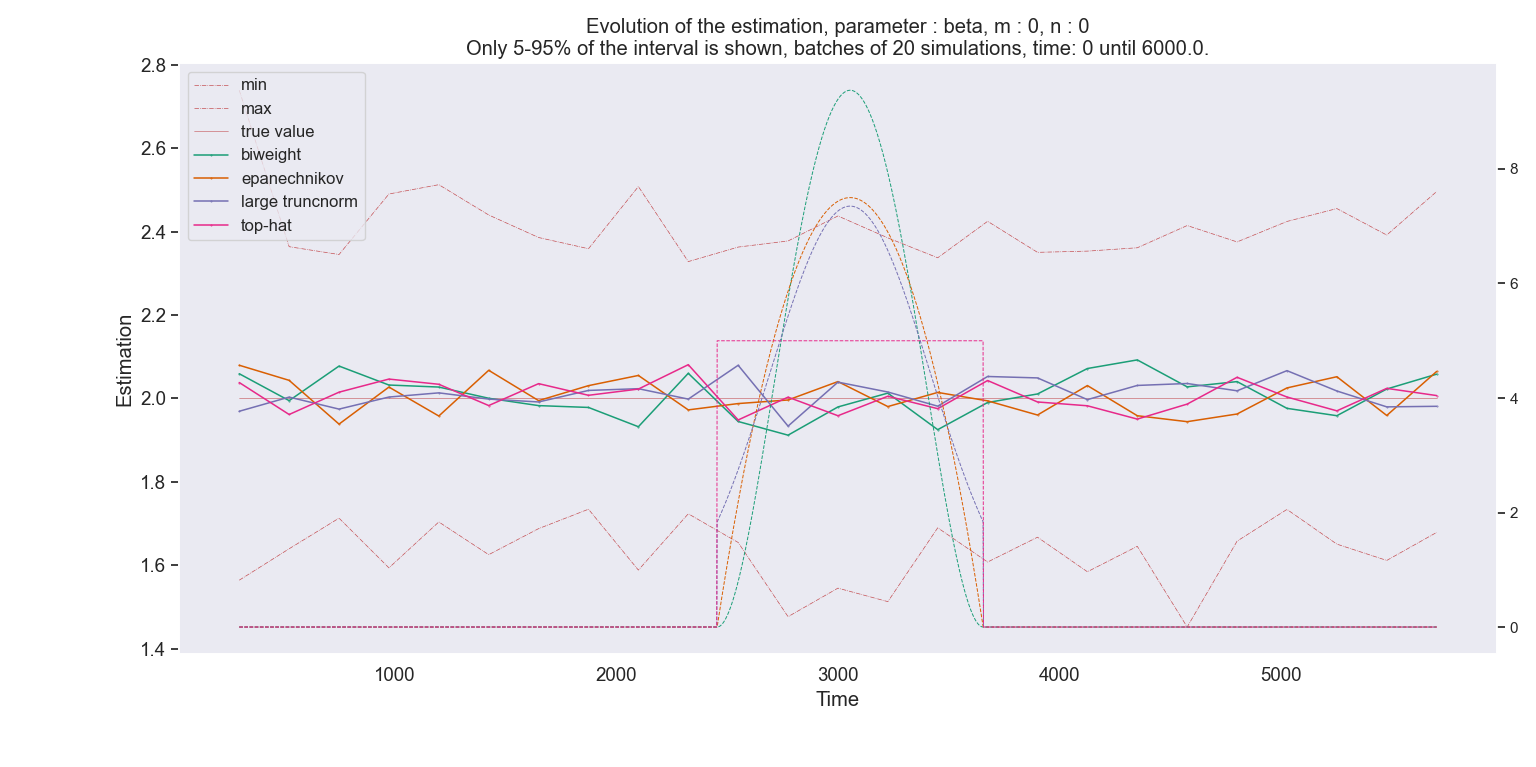
\includegraphics[width = 0.90 \textwidth]{../imag/chap3/compar_kernel/beta.png}
\caption{Fixed kernel density estimation, showing the impact of the type of kernels. Plot of beta.}
\label{fig:basic_5_kernels_beta}
\end{figure}

\begin{figure}
\centering
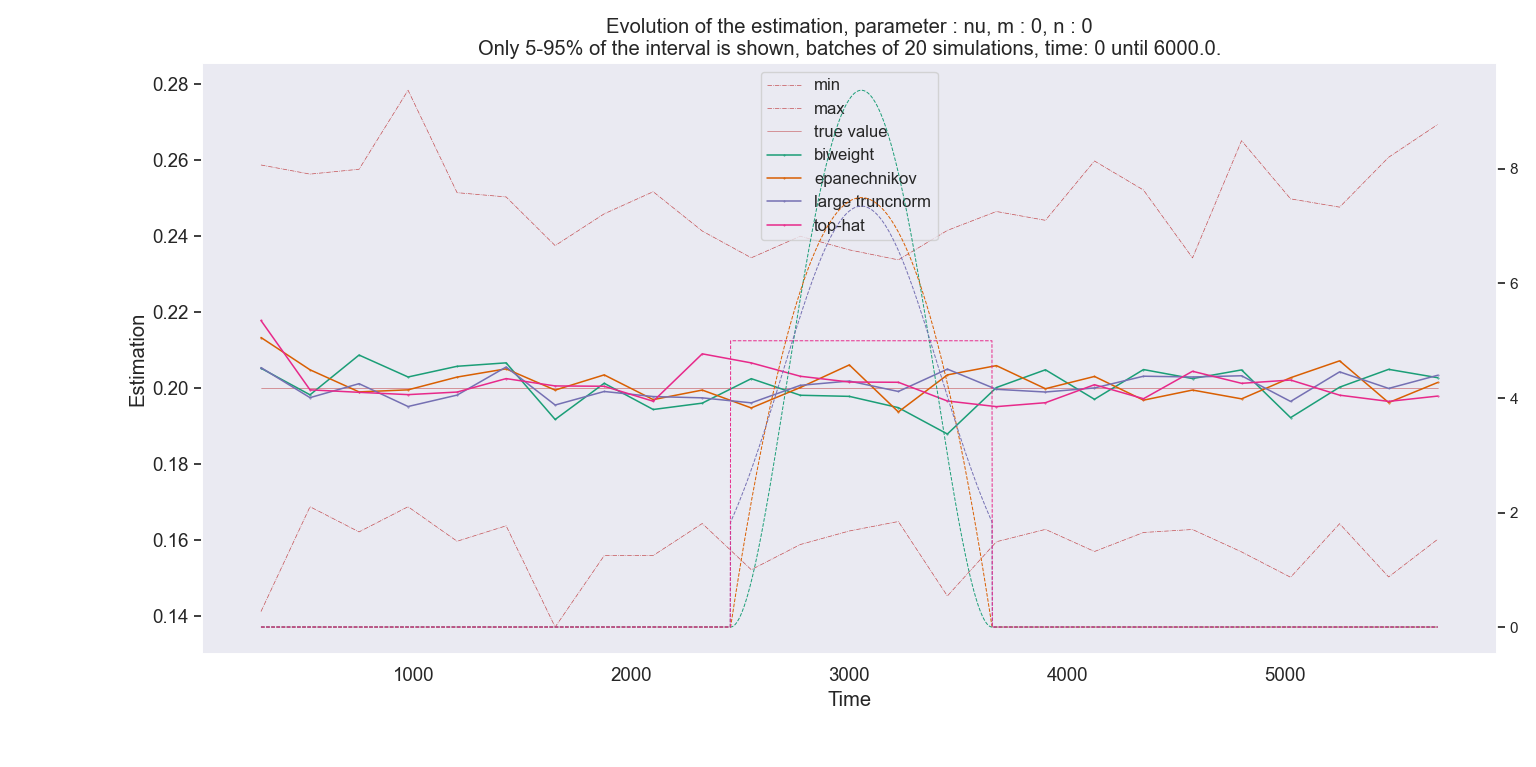
\includegraphics[width = 0.90 \textwidth]{../imag/chap3/compar_kernel/nu.png}
\caption{Fixed kernel density estimation, showing the impact of the type of kernels. Plot of nu.}
\label{fig:basic_5_kernels_nu}
\end{figure}







\subsection{Optimal Width}
\label{subsection:optimal_width}


The optimal width derived within the theory of KDE is not relevant for our concern. The estimator $\widehat{\theta}$ is taken as a function of the kernels:

$$ \hat{f}(x) := \frac 1 {n h} \sum^n K \left ( \frac{x - X_i } {h}  \right )$$

where $n$ is the number of data you have, $h$ the window's width. However, in our case, the kernel is shaping the data given to the MLE and so the relationship between the estimate and the kernels is more complicated.


Since we weren't able to determine a simple relationship, we recommand chosing a meaningful width for the first optimal width. A good first blind guess can be $1/5$ of the total length of observations. The more the parameters are varying with respect to time, the smaller the width should be. That first guess about the shape of the functions driving the parameters is perhaps the most meaningful first optimal width.

\begin{remarque}
One should be careful about not having too narrow kernels. If the algorithm doesn't have enough data to observe, the MLE might fail to converge.
\end{remarque}

We observe the impact of the width here in fig. \ref{fig:basic_3_kernels_alpha}, \ref{fig:basic_3_kernels_beta}, \ref{fig:basic_3_kernels_nu}. We compare the same size as the previous figures with twice and half as wide. We observe that the smallest kernels yields the more variable estimates.

\begin{figure}
\centering
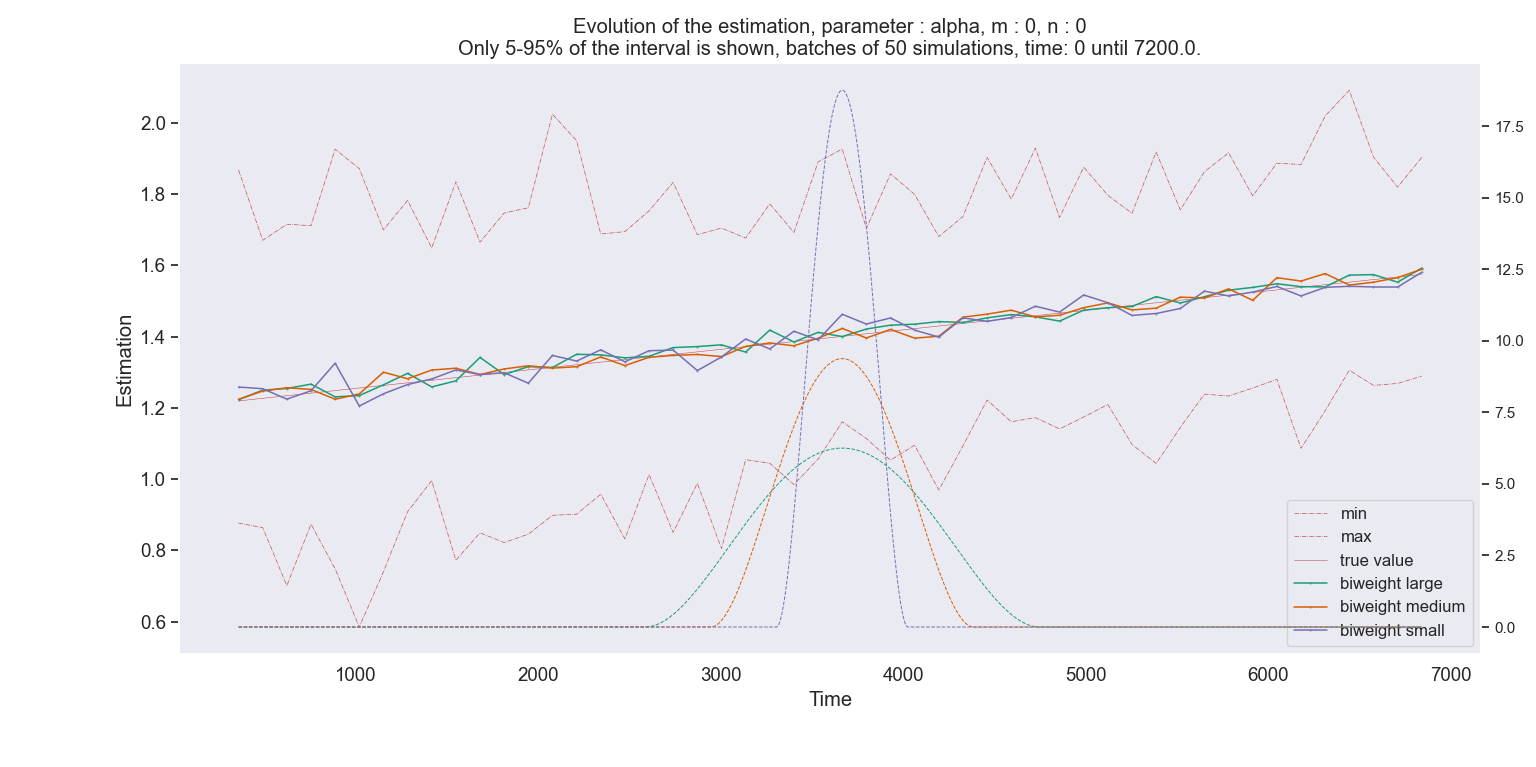
\includegraphics[width = 0.90 \textwidth]{../imag/chap3/compar_kernel/3alpha.png}
\caption{Fixed kernel density estimation, showing the impact of the width of the biweight kernel. Plot of alpha.}
\label{fig:basic_3_kernels_alpha}
\end{figure}

\begin{figure}
\centering
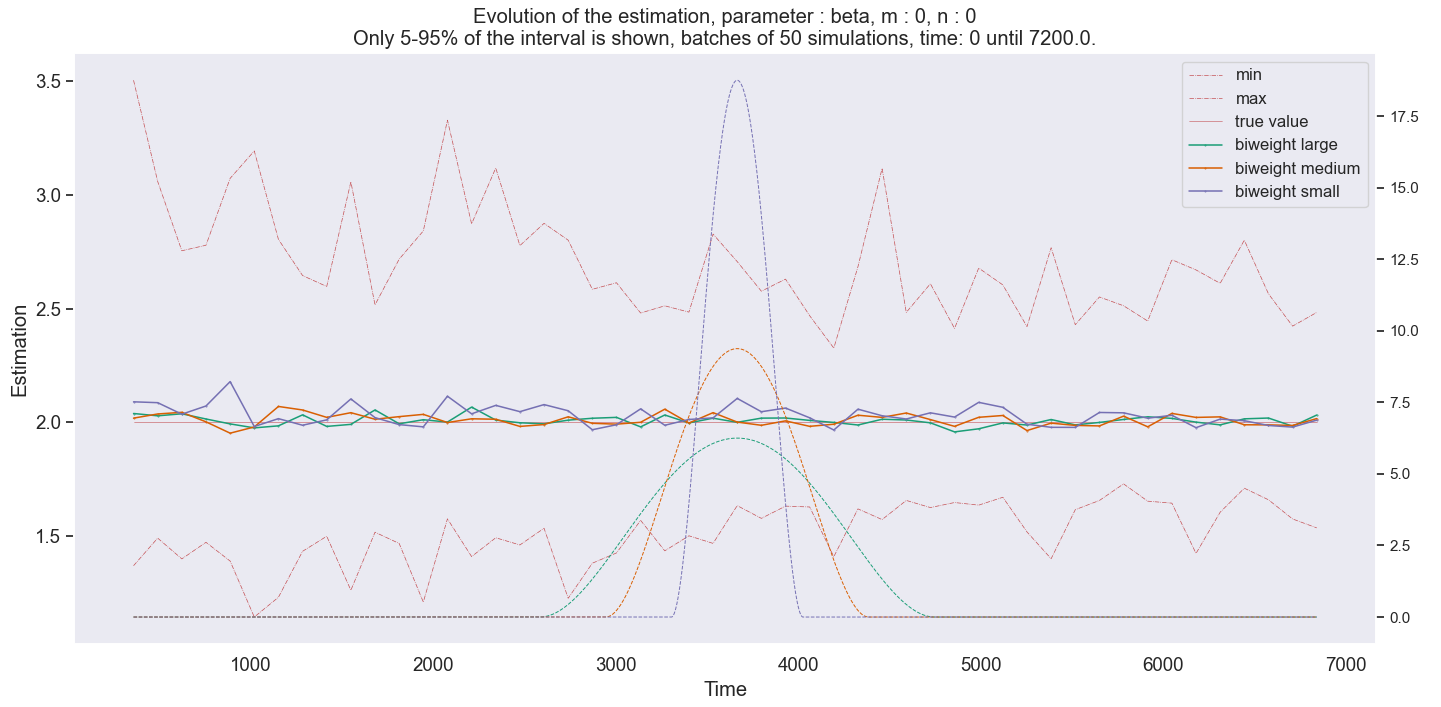
\includegraphics[width = 0.90 \textwidth]{../imag/chap3/compar_kernel/3beta.png}
\caption{Fixed kernel density estimation, showing the impact of the width of the biweight kernel. Plot of beta.}
\label{fig:basic_3_kernels_beta}
\end{figure}

\begin{figure}
\centering
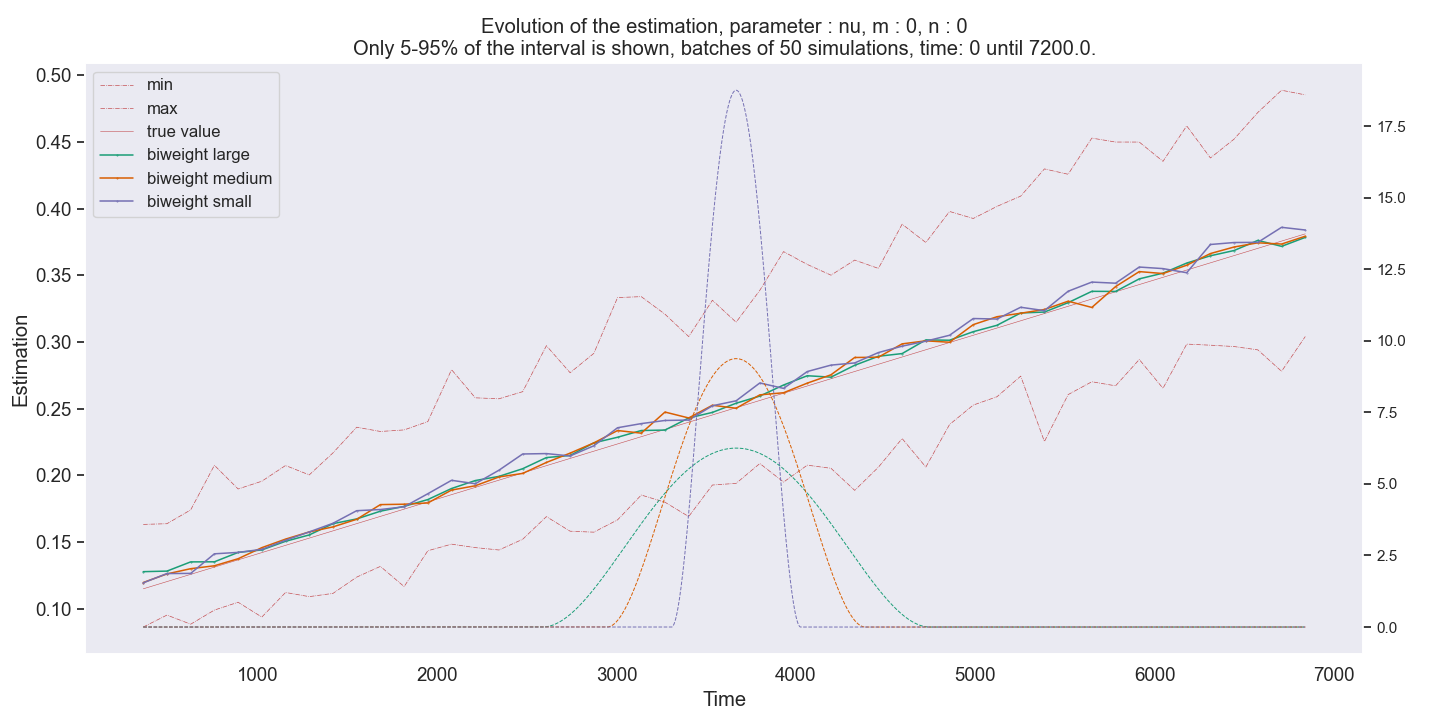
\includegraphics[width = 0.90 \textwidth]{../imag/chap3/compar_kernel/3nu.png}
\caption{Fixed kernel density estimation, showing the impact of the width of the biweight kernel. Plot of nu.}
\label{fig:basic_3_kernels_nu}
\end{figure}




\section{Adaptive Width Window}
\subsection{Idea Behind AKDE}
Another method is called the Adaptive Kernel Density Estimation (AKDE). The author refers to \cite{Methods_ESTIM} and \cite{AKDE_ex} for more details. We synthesize the method.


Adaptive Width Window kernel estimation lies upon the idea that we are going to estimate the function through a two-step process. The first step is giving a rough estimate named the pilot estimate. Strong of that first estimate, one rescales kernels' width with respect to the geometric metric. Geometric mean has the property of being very sensible to small number. Scaling by comparing the value to the geometric mean is then a way to boost the evolution of relatively extremal values. 
Then, the second step is using the new constructed kernels in order to create a good estimate.



\subsection{Algorithm for AKDE}
\label{section:algo_awke}
The geometric mean for a sequence $\sequence{ a_i } $ is commonly defined as $$ G_{a} := \left (  \prod^n a_i \right  )^{\frac 1 n }$$ and we define the sensitivity parameter satisfying $ 0 \leq \gamma \leq 1$. It is quite common to set $\gamma = \frac 1 2$; this value can be found in the book \cite{Silverman} or in the article \cite{abramson}. Then we have:
\begin{equation}
\label{eq:local_width_factor}
\forall t_i \in \sequence{t_i}, \qquad \lambda_{t_i} :=  \left ( \frac{\widetilde{f}(t_i) }{G_{\widetilde{f_i}} } \right ) ^{ - \gamma }  
\end{equation}

and  $ G_{\widetilde{f_i}} $ is based upon the sequence $ \sequence{ \widetilde{f}(t_i) } $






\begin{algorithm}[H]
\label{algo:adaptive1}
\SetAlgoLined
1. \quad Find a pilot estimate coined $\widetilde{f}$. We use the optimal kernel from section \ref{section:FWW}, which for a kernel $K^*$ and a bandwidth $h^*$ is of the form $$ (t, t_i) \to \frac 1 {h^*} K^* \left ( \frac{t - t_i}{h^*} \right ) $$ 

2. \quad $\forall t_i \in \sequence{t_i}$, when we estimated the pilot estimate $\widetilde{f}$, create the local width factor $\lambda_{t_i}$ according to eq. (\ref{eq:local_width_factor}). 

3. \quad Find the final estimate $\hat{f}$ by using a different kernel for each $t_i$. $\forall t \in \sequencetime $, the new kernel shall be of the form:
$$ (t, t_i) \to \frac 1 {\lambda_{t_i} h^*} K^* \left ( \frac{t - t_i}{\lambda_{t_i} h^*} \right )$$ 
\caption{Adaptive Kernel Estimation}
\end{algorithm}












\begin{remarque}
The interpretation of the scaling coefficient $\sequence{\lambda_{t_i}}$ can be stated like that. The bigger the coefficient, the more the bandwidth is scaled up. A coefficient smaller than one is equivalent to a pilot value bigger than the geometric mean. In other words, $\gamma$ is increasing the discrepancy of the first optimal estimate. Hence, when the estimate is relatively smaller (resp. bigger), the kernels get wider (resp. tighter). 

Essentially, such kernels are useful for KDE since places with estimated high density get narrower kernels for a more precise estimation while other intervals with low density, mainly the tails, observe wider kernels that capture the potential smooth decay of the density. 
\end{remarque}



In order to compute the geometric mean in an optimized way in python, one can use:

\begin{verbatim}
from scipy.stats.mstats import gmean
gmean( [np.array] )
\end{verbatim}

In particular, a classic problem for large arrays is overflow. A good habit is to map the array to a log-domain first, calculate the sum of these logs, then multiply by $\frac 1 n$ and finally calculate the exponential. Here I give two hand-written functions in order to compute the same result:

\begin{verbatim}
def geo_mean(iterable):
    a = np.array(iterable)
    return a.prod()**(1.0/len(a))
\end{verbatim}    
\begin{verbatim}
def geo_mean_overflow(iterable):
    a = np.log(iterable)
    return np.exp(a.sum()/len(a))
\end{verbatim}



\begin{figure}
\centering
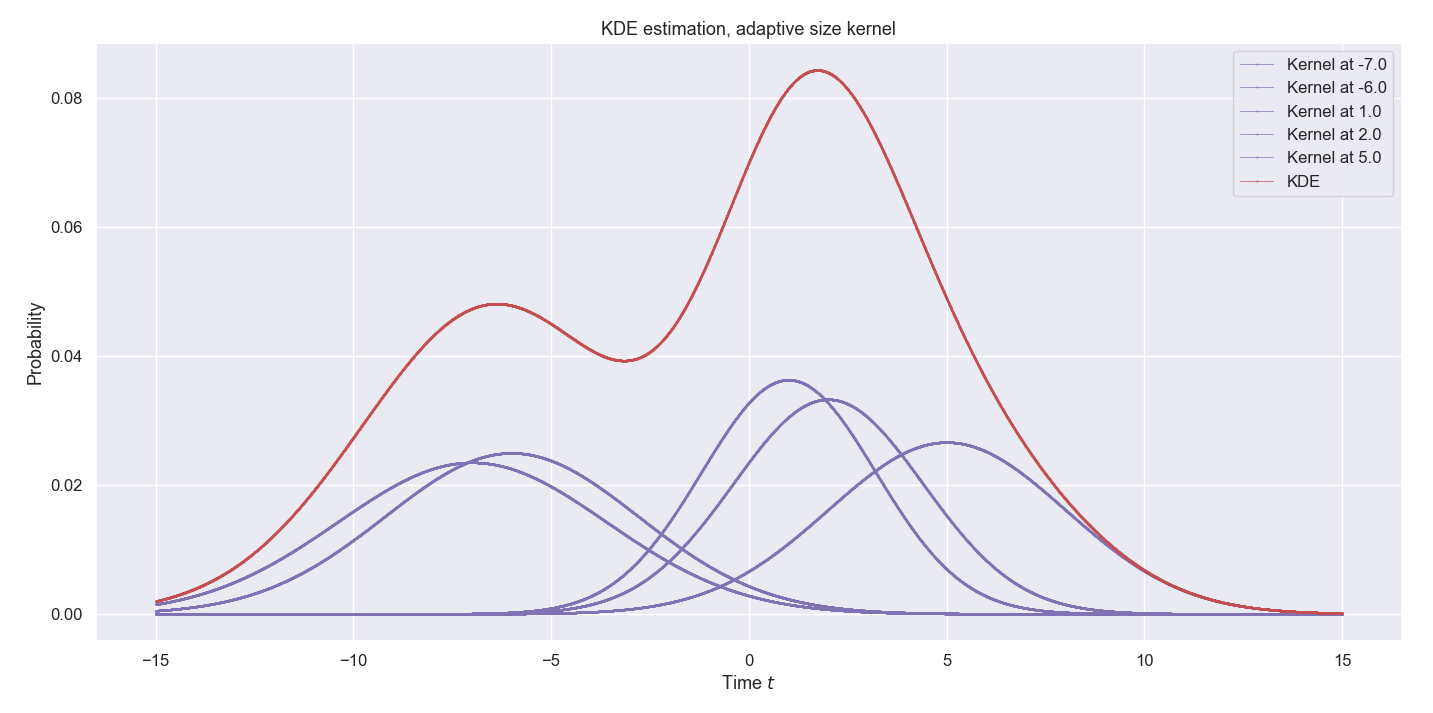
\includegraphics[width = 0.90 \textwidth]{../imag/chap3/AKDE.png}
\caption{The adaptive kernel density estimation, after the second step. Same points as on fig. \ref{fig:FKDE}), we observe how the kernels changed through the computations as well as the impact of the single kernels on the KDE.}
\end{figure}







\subsection{Equivalence Between Representation of Kernels}
\label{section:equivalence_bi_rep}

In the theory of kernels, most of plots show how one can find an estimate of a density by summing up rescaled-centred kernels, and plots like the left one from fig. \ref{fig:CKDE} are rampant. One should notice that it is also totally equivalent to represent KDE as the right picture. The rescale put aside, a kernel is a two-dimensional function: 

\begin{equation*}
(t,t_i) \to K(t - t_i) 
\end{equation*}

The left graph from fig. \ref{fig:CKDE} shows the function 
$$ \forall t \in \R, \ (t,t_{ \{1,2,3 \} }) \to K(t- t_{ \{1,2,3 \} }) $$ 
for three different $t_i$; the right one shows the function
$$ \forall t_i \in \sequence{ t_i }, \ (0,t_i ) \to K(0 - t_i) $$ 
and the stars corresponds to values we add up in order to get the estimate in $0$, when one uses $\hat{f}(t) = \sum_i K(t-t_i)$. 

This has an interesting implication. One can think about kernels as a function of one parameter and this will give a different representation of the situation depending which we chose. In the author's opinion, the second representation, from fig. \ref{fig:CKDE}, is more intuitive and efficient for our weighting problem. 

\begin{itemize}
\item Indeed, it is very \textbf{intuitive} to see the point $t$ as the point when we search for an estimate, and observe the shape of the kernel impacting the data upon it. 
\item It is also very \textbf{efficient} when one uses it with adaptive kernel estimation. The previously introduced algorithm used in KDE is based upon the first representation and thus considers the kernels as function of time. Hence, in the first representation from fig. \ref{fig:CKDE} we are scaling $\# \sequence{t_i}$ kernels, where $\#$ denotes the number of elements of the sequence. On the other hand, the other representation asks for rescaling $\#\sequencetime$ kernels. 
\end{itemize}


In the end, this double representation comes from the nature of the used kernel. We are using transition probabilities (transition kernels) which can be defined as:

\begin{definition}[Transition Kernel]
Let $(\Omega, \mathcal F), ( \mathcal X, \mathcal B (X) )$ two measurables spaces. Then $$ \kappa : \mathcal F \times \mathcal B (X) \to [0, \infty] $$ is called a kernel from $\mathcal F$ to $\mathcal B(X)$ if and only if:

\begin{itemize}
\setlength{\itemindent}{3. cm}
\item $\forall B \in \mathcal B(X), t \to \kappa(  t, B)$ is measurable
\item $\forall t \in \mathcal F, B \to \kappa(  t, B)$ is a measure.
\end{itemize}
\end{definition}

Then, one can see the previously stated $K$ or $w$ as the unidimensional case of transition kernels. Notice, we could rewrite eq. (\ref{eq:weighted_log_likelihood}) in the following way:

$$ \ln W L^m( \Theta \mid \Tau ) = - \int_0^T \lambda^{m} ( s \mid \Theta , \Tau ) \kappa(t, ds) + \int_0^T \ln \lambda^{m} ( s \mid \Theta , \Tau^m ) \kappa(t, d N_s)  $$

\begin{figure}
\centering
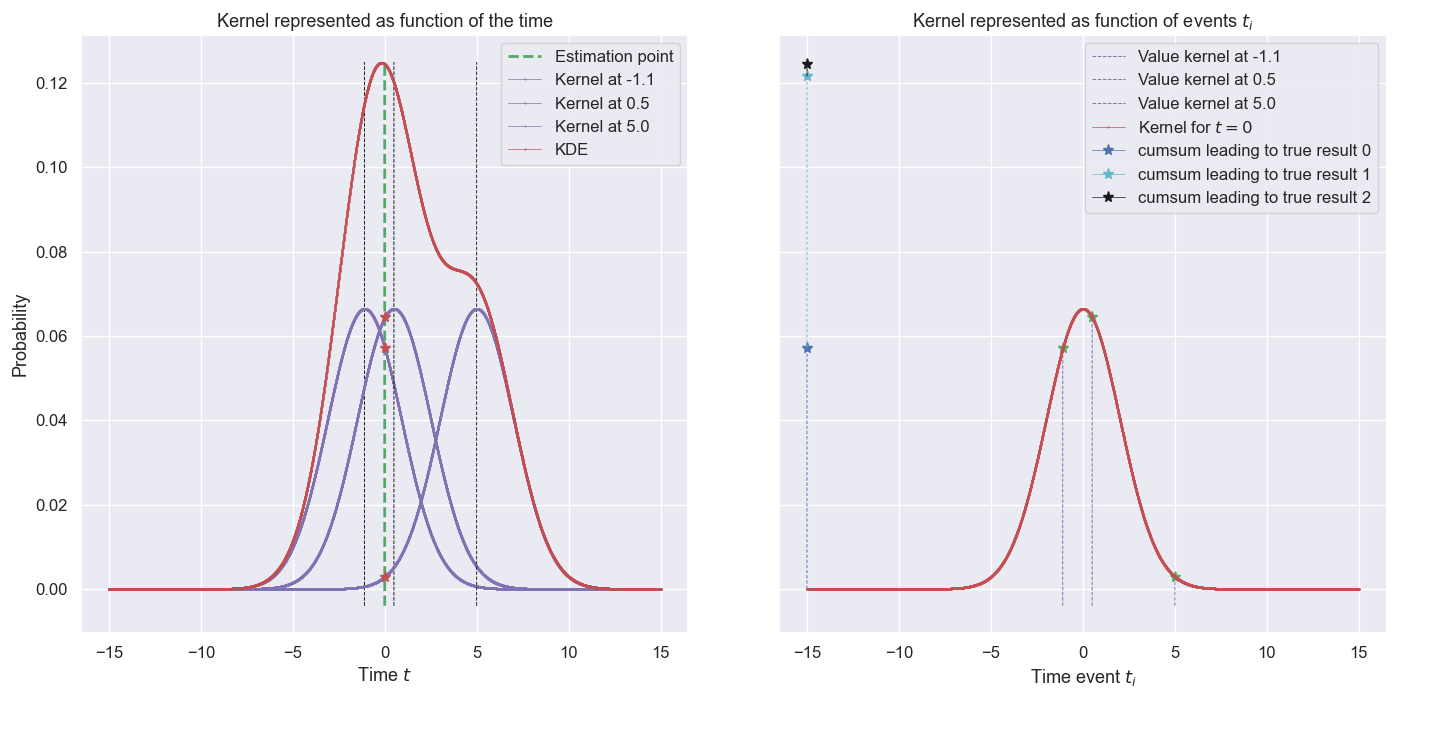
\includegraphics[width = 1.00 \textwidth]{../imag/chap3/CKDE.png}
\caption{Comparison of the two equivalent representations for symmetric kernels.}
\label{fig:CKDE}
\end{figure}

\begin{figure}
\centering
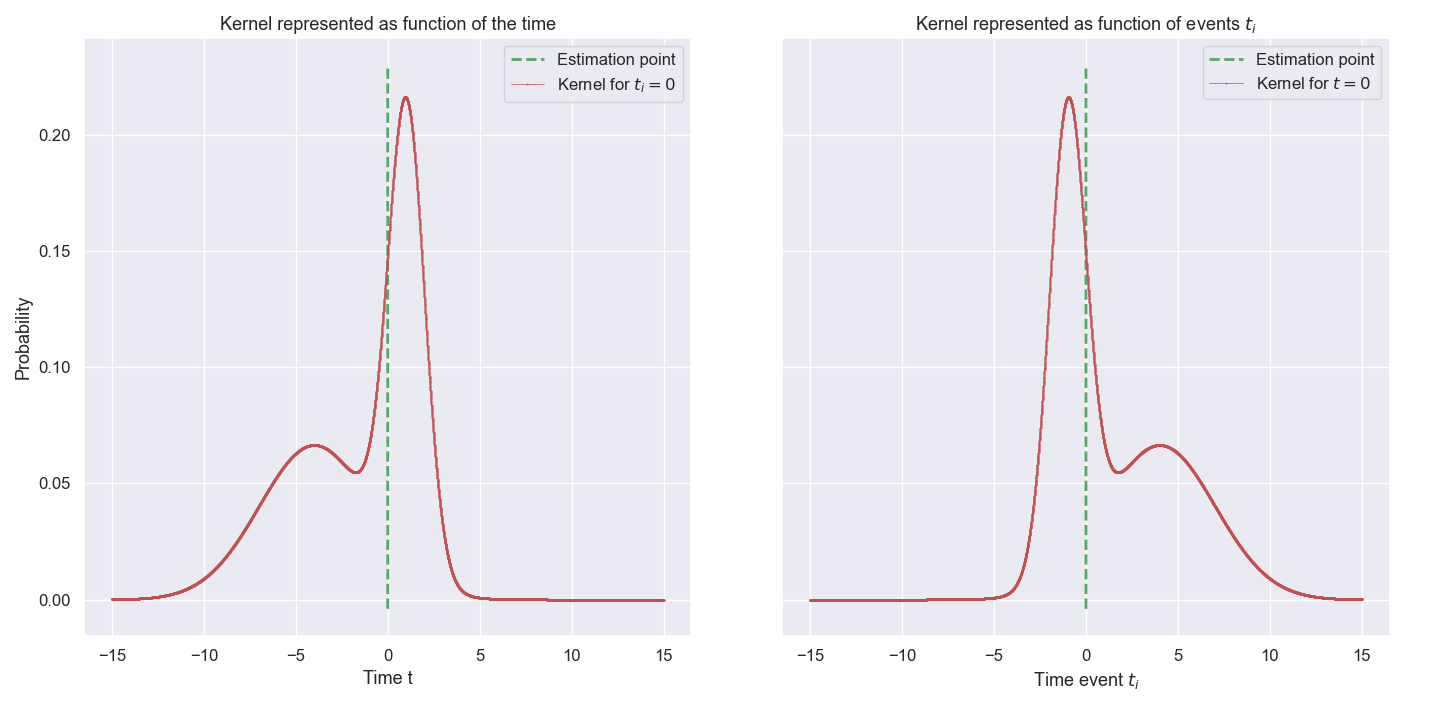
\includegraphics[width = 1.00 \textwidth]{../imag/chap3/CKDE2.png}
\caption{Comparison of the two equivalent representations for asymmetric kernels.}
\label{fig:CKDE2}
\end{figure}

\willlastcheck{check that the newpage is ok.}

\newpage 
Finally, one shouldn't jump from one representation to another without some precautions. The equality $K(t - t_i) = K(t_i - t)$ holds if and only if $K$ is even. Then, though our equivalence from fig. \ref{fig:CKDE} was suggesting the usage that we plotted the same function on both plots (resp. in purple on the left and in red on the right), it is clear on fig. \ref{fig:CKDE2} that it is not the case. For that reason, the author offers to conclude the discussion we started at the end of section \ref{section:kernel_weights_first_conversation}. We wrote down the following definitions as being the main distinction between kernels and weights, which also grants some unification between the two representation:
\begin{definition}[Kernel]
$K$ is a scaled function of the time, with as parameter the jump's time $t_i$.
\end{definition}

\begin{definition}[Weight function]
$w$ is a function of the jump's time, with as parameter time $t$.
\end{definition}

\begin{theoreme}[label = thrm:equiv_w_k]{Equivalence weights and kernels}
The two definition are linked through those equalities
\begin{align*}
\forall t \in \sequencetime, \ t_i \in \sequence{t_i }, \qquad w_t(t_i) 
&= w(t_i - t) \\
&=  K(t - t_i) \cdot \norm{w}_{L^1} \\
&= K_{t_i}(t) \cdot \norm{w}_{L^1}
\end{align*}
\end{theoreme}





\section{Improvement of the AKDE}
\subsection{A New Scaling Function}


\begin{figure}
\centering
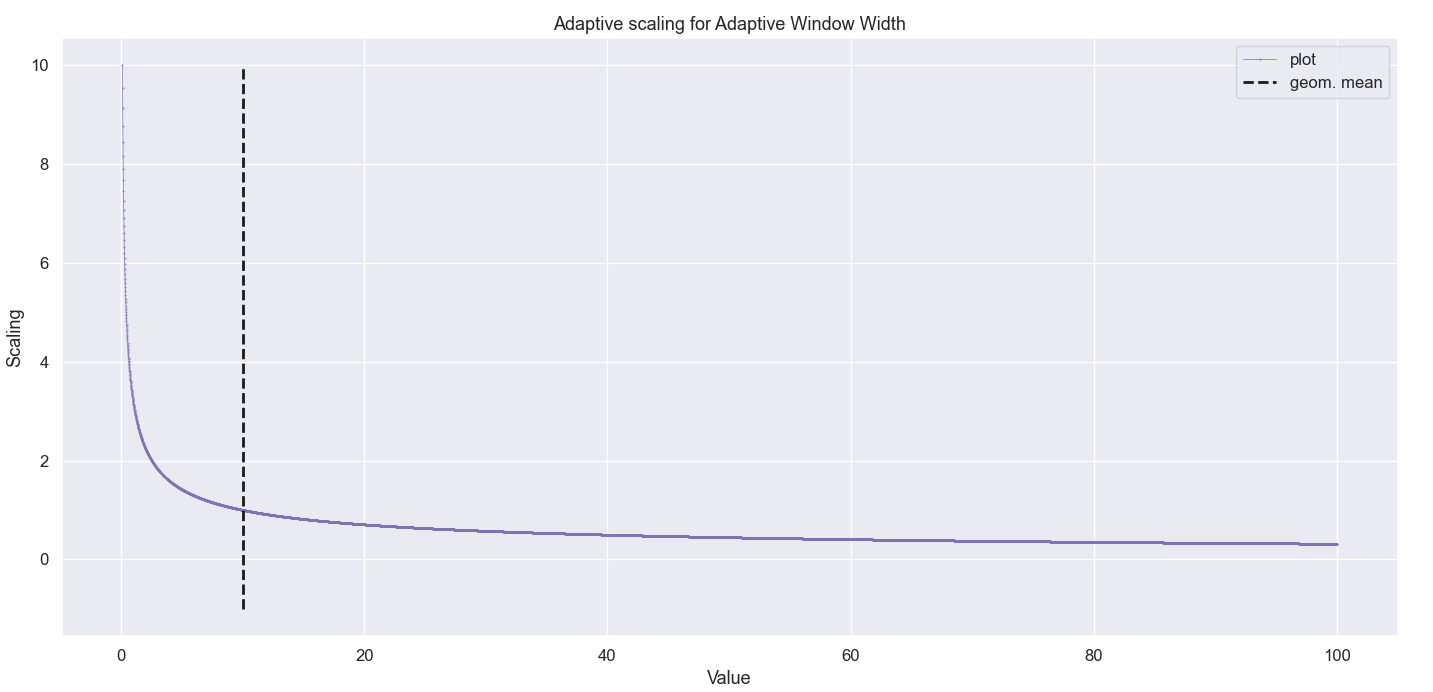
\includegraphics[width = 0.95 \textwidth]{../imag/chap3/old_funct.png}
\caption{Plot of the previously presented function $g$ in eq. (\ref{eq:local_width_factor}) as well as in equation (\ref{eq:old_g}). We plot it as a function of the first estimate's result.}
\label{fig:old_scaling}
\end{figure}


\begin{figure}
\centering
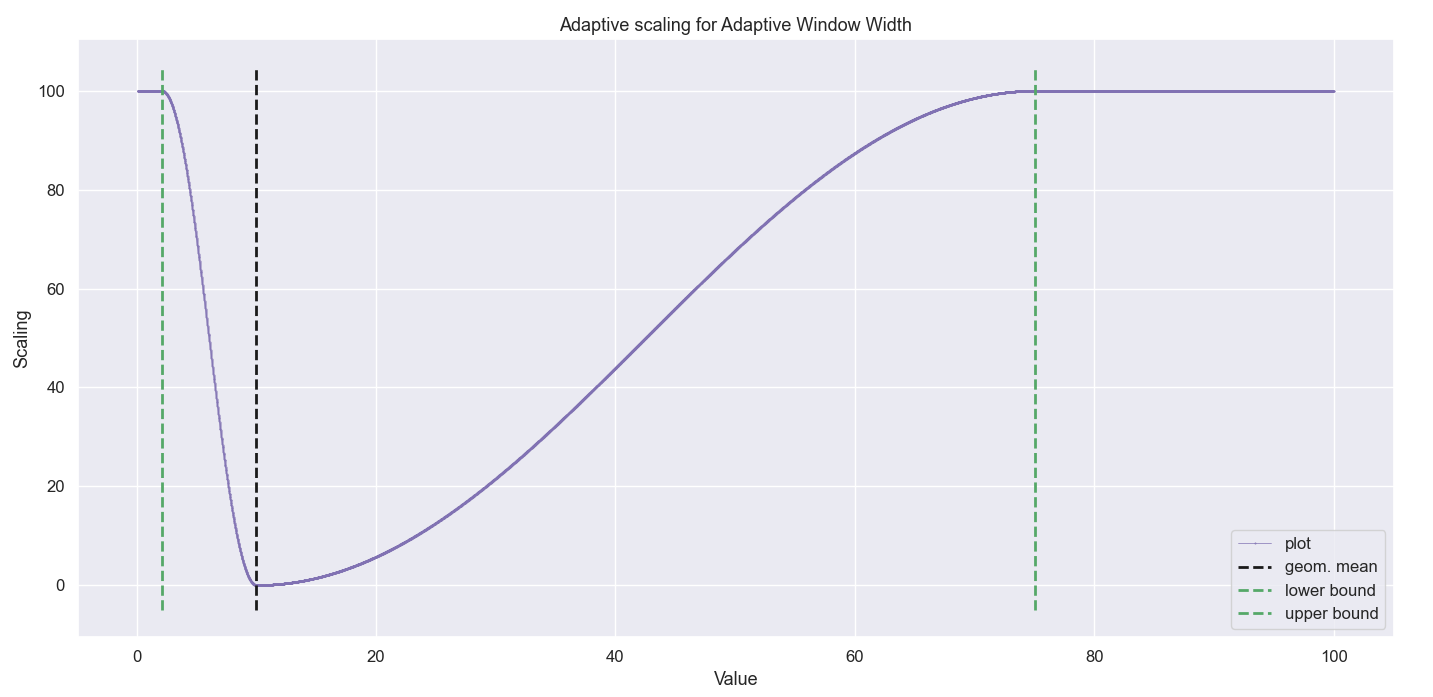
\includegraphics[width = 0.95 \textwidth]{../imag/chap3/my_new_funct.png}
\caption{Scaling output depending on how close the estimate is to the geometric mean. The lower branch ends at $2$, the mean is $10$ and the upper branch finishes at $75$. We constructed the function as a two sinusoidal branches function.}
\label{fig:new_scaling}
\end{figure}

In the previous algorithm, the kernels are scaled with respect to the geometric mean. In particular, high probability points get narrower kernels, and low probability points get wider kernels. This is not the expected behaviour for our task. We would like to scale extremes, while broadening points at the medium.



This is the reason why the author wanted to improve the rescale system of the AKDE. Notice that the idea of the algorithm is to rescale the kernels based upon a function $g$, which takes as parameters one element of an array and the geometric mean. 

The originally used $g$ function can be written like eq. (\ref{eq:old_g}) and is plotted for $G = 10$, $\gamma = 1/2$ on fig. \ref{fig:old_scaling}. 

\begin{equation}
\label{eq:old_g}
g(x,G, \gamma) =  \left ( \frac x G \right ) ^{-\gamma}
\end{equation}

We call the function $g$ the rescale function. We want to find a better rescale function, that suits better our needs. We propose the following function:


\begin{theoreme}[label = thrm:new_g]{New $g$ rescale function}
\begin{align}
\label{eq:new_g}
g(x, G, L,R,h,l) &=   \frac {h-l} 2 \left (2 
-  \11charac_{ [- \pi, 0]} (u)  \cos(u)
-  \11charac_{ [0, \pi]} (v)  \cos(v) \right ) + l,  \\
\quad & u = \frac{x - G}{G- L} \pi, \notag  \\
\quad & v = \frac{x - G}{R- G} \pi \notag
\end{align}

where $G$ shall correspond to the geometric mean of the pilot estimate, $L$ (resp. $U$) is taken in the following as the $0.02$-quantile (resp. $0.98$-quantile). $h,l$ are added as the parameter of scaling.
\end{theoreme}



Recall that $p$-quantile for an ordered serie of length $n$ is defined as being equal to its $\lceil{np}\rceil$-value\footnote{$\lceil{\cdot}\rceil$ is the ceil-function.}.


What has been done here is that we created on a function that:



\begin{itemize}
\item equals to $l$ in $G$, 
\item behaves smoothly along the line, quadratically near the ends of the branches and linearly in the middle (since it is a cosinus),
\item equals $h$ for extreme values,
\item is easily adaptable to the first estimation, by modifying $L$ and $R$,
\item through the substitution $u,v$, one can easily interpret R and L as the values at which the branches are reaching their final values. Choosing L and R as quantiles allows the user to choose how much data is considered as extreme. 
\end{itemize}

\begin{remarque}
We recommand taking $h$ as $2.5$, $l$ as $0.2$; $L$ as the $2$-quantile and $R$ as $98$-quantile. Those values worked very well for us.
\end{remarque}

One can see how the function $g$ looks like on fig. \ref{fig:new_scaling}. We offer here one implementation in python:


\begin{verbatim}
def mean_list(my_list):
    # the default behaviour if list is empty, it returns 0.
    return float(sum(my_list)) / max(len(my_list), 1)
    
    
def my_rescale_sin(value_at_each_time, L=None, R=None, h=2.5, l=0.2 / 2, silent=True):
    if any(value_at_each_time != 0):
        # I compute the geometric mean from our estimator.
        G = gmean(value_at_each_time)

    else :  # G == 0, it happens if no norm computed.
    #then it has to return 0.01 such that it widen all the kernels.
        return np.full(len(value_at_each_time), 0.01)

    if L is None:
        L = np.quantile(value_at_each_time, 0.02)
    if R is None:
        R = np.quantile(value_at_each_time, 0.98)

    if not silent:
        print("Left boundary : ", L)
    if not silent:
        print("Right boundary : ", R)

    xx = value_at_each_time - G

    ans = 0
    scaling1 = math.pi / (G - L)
    scaling2 = math.pi / (R - G)
    # I fix the part outside of my interest, to be the final value, h.
    # This part corresponds to math.pi.
    # I also need the scaling by +h/2 given by math.pi

    # xx2 and xx3 are the cosinus, but they are different cosinus.
    # So I fix them where I don't want them to move at 0 and then I can add the two functions.
    my_xx2 = np.where((xx * scaling1 > -math.pi) & (xx * scaling1 < 0),
                      xx * scaling1, math.pi)  # left
    my_xx3 = np.where((xx * scaling2 > 0) & (xx * scaling2 < math.pi),
                      xx * scaling2, math.pi)  # right
    ans += - (h - l) / 2 * np.cos(my_xx2)
    ans += - (h - l) / 2 * np.cos(my_xx3)

    ans += l  # avoid infinite width kernel, with a minimal value.
    return ans
\end{verbatim}


\begin{remarque}
We notice that chosing the quantiles as $2$ and $98$ isn't too extreme. The function $g$ is flat on the sides and though having only $4\%$ of the values being considered as extrems is low, the number of points having the kernels narrowed is actually much bigger in practice. Putting $10-90$ did actually yielded half of the kernel being narrowed extremely.
\end{remarque}

\subsection{Is The Rescale Function Well-Defined ?}

\willprecise{ do a better job here }


That question is left to the reader. As a hint, we thought about the following inequalities, which hold for any sequence of positive numbers $\sequence{a_i}$:
\willlastcheck{ Good position of the inequalities }
\begin{alignat}{2}
\text{Harmonic Mean} 
&\leq \text{Geometric Mean} 
&& \leq \text{Arithmetic Mean} \notag \\
\frac n {\sum^n \frac 1 {a_i} } 
& \leq \hspace{0.55 cm} \left ( \prod^n a_i \right ) ^{ \frac 1 n } 
&& \leq \frac 1 n \sum^n a_i \notag
\end{alignat}
where the equality holds when the sequence is constant.

The function $g$ should be well defined. An issue might arise if some values were negatives, but in our study, we deal with self-exciting Hawkes processes whose parameters are all positive (as well as we are computing the $l^2$ norm). Another concern is, when do we have $L \leq G \leq R$? This is fundamental for the function to be well behaved. For now, the user should check by hand.


\willdo{ peut etre ailleurs cette section.}



















\section{From KDE to WMLE}

We mentioned throughout our study that though we summarize methods about KDE, it is actually possible to use the same methods for weighted maximum likelihood estimation. Let's go through the small necessary adjustments again.

\subsection{From Kernels to Weights}
As mentioned in section \ref{section:kernel_to_weights}, as well as through theorem \ref{thrm:equiv_w_k}, in order to go from the kernels of the theoretical part of this chapter to the space $\Omega_w$ as defined at the beginning of the chapter, one simply has to multiply by a constant, equal to the total considered time of simulation. Thus, we have the equality:

$$ T \cdot K ( \cdot ) \equiv w ( \cdot ) $$

\subsection{From One-Dimensional Kernel to Multi-Dimensional Statistics}
As mentioned in section \ref{section:multi_to_uni}, another issue lies in the fact that we can't compute the geometric mean of $\theta^*_{\cdot} \in \mathbb R^{m+2m^2}$ for the algorithm from section \ref{section:algo_awke}\footnote{By $\theta^*_{\cdot}$ we mean the function $\theta^*$, evaluated at an unknown point. The function corresponds to the estimate of the WMLE, which is a function of time because of the time dependence of the involved weights.}.
However, one can apply the geometric mean on the norms of the estimators. By default, one can use the $l^2$ norm of $\theta^*_{\cdot}$, in other words

$$\theta = (\theta_1, \theta_2, \cdots, \theta_n ) \implies 
\norm{\theta}_{l^2} = \left ( \sum^n_1 \theta_i^2 \right )^{\frac 1 2}$$ 

Please remember that in our case, $\theta$ is time dependant so taking the norm over $\theta$ recovers a function from $[0,T]$ to $\R$. Hence, if we allow $t$ to take only certain given values, $\norm{\theta_t}_{l^2}$ can be seen as a sequence.


\begin{remarque}
A particular care of scaling the parameters should not be skipped. Indeed, not scaling the parameters could lead to the classic problem of data-sciences related to feature normalization. The features with high magnitudes will weigh in a lot more in the distance calculations than features with low magnitudes, in particular for euclidean distance.
\end{remarque}

\subsection{Scaling}
\label{subsection:scaling}

As mentioned in the previous subsection, we might have to apply some scaling to the estimates. We chose a classical positive mean-scaling:

$$ \forall i \in  \llbracket 1, M \rrbracket, \qquad  \widetilde{\theta_i } = \frac{\theta_i - \mean \theta }{\max(\theta) - \min(\theta) } + 1 $$

It makes sense as we care about how the values are extremes in comparison to each others. The scaling is also linear and thus does not change essentially the distribution\footnote{Unlike normalization.}. The classical mean-scaling does not involve the additional $+1$, and its values lie in $[-1,1]$. The shift ensures a positive value, which is very important in order to keep the order of norms: minimals norms for low estimation; maximal norms for high estimation.


A problem appear with non-moving parameters. Worst case scenario is when there is no change for a parameter. Then, the time series of means is showing no autocorreletion and the plot is essentially noise. Furthermore, it is quite common to observe some strong correlation in between the parameters (alpha goes up, beta goes up as well) exagerating the change in the kernels width. A solution we implemented is to not considere the evolution of parameters with no significant change. Our criterea is a minimal percent change with respect to the original (at time 0) value of the parameter. The default minimum is $10\%$ though it can be changed.


We offer here an implementation of what we just said. 

\begin{verbatim}
def rescale_min_max(vect):
    the_max = max(vect)
    the_min = min(vect)
    the_mean = classical_functions.mean_list(vect)
    ans = [(vect[i] - the_mean) / (the_max - the_min) + 1 for i in range(len(vect))]
    return ans


def check_evoluating(vector, tol):
    ''' if all values of the vector are inside the tube mean +/- tol, return false.
    Args:
        vector:
        tol:

    Returns:

    '''
    the_mean = classical_functions.mean_list(vector)
    if all(element < the_mean * (1 + tol) for element in vector) and all(
            element > the_mean * (1 - tol) for element in vector):
        return False
    return True


def rescaling_kernel_processing(times, first_estimate, considered_param, tol=0, silent=True):
    # on the first entry, I get the time, on the second entry I get nu alpha or beta, 
    #then it s where in the matrix.
    # considered_param should be which parameters are important to consider.

    # ans is my vector of normes. Each value is for one time.
    ans = np.zeros(len(times))

    # times and first_estimate same length.
    # I need to pick the good parameters and rescale them accordingly.

    # the dimension of the data.
    M = len(first_estimate[0][0])
    total_M = 2 * M * M + M
    include_estimation = [False] * total_M
    # I am creating a vector with 2M*M + M entries,
    #each one is going to be scaled, and this is the parameters I am using afterwards.
    vect_of_estimators = [[] for _ in range(total_M)]
    for k in range(len(times)):
        for i in range(M):
            vect_of_estimators[i].append(first_estimate[k][0][i])
            for j in range(M):
                vect_of_estimators[M + i + j].append(first_estimate[k][1][i][j])
                vect_of_estimators[M + M * M + i + j].append(first_estimate[k][2][i][j])

    for i in range(total_M):
        # check the parameters I need to check.
        if i < M and 'nu' in considered_param:
            include_estimation[i] = True
        elif i < M + M * M and 'alpha' in considered_param:
            include_estimation[i] = True
        elif 'beta' in considered_param:
            include_estimation[i] = True

        if include_estimation[i]:
            if not check_evoluating(vect_of_estimators[i], tol):  # we don't keep the True
                include_estimation[i] = False
    if not silent:
        print("which dim to include for norm : ", include_estimation)

    rescale_vector = []
    for i in range(total_M):
        if include_estimation[i]:
            rescale_vector.append(rescale_min_max(vect_of_estimators[i]))

    for j in range(len(times)):
        ans[j] = np.linalg.norm(
        [rescale_vector[i][j] for i in range(len(rescale_vector))], 2)
    # I compute the geometric mean from our estimator.
    G = gmean(ans)
    if not silent:
        print("vect  :", vect_of_estimators)
        # print("interm :", rescale_vector)
        print("the norms ", ans)
        # print('mean : ', G)
    scaling_factors = my_rescale_sin(ans, G=G, silent=silent)
    return scaling_factors
\end{verbatim}

\subsection{Number of Kernels to Rescale}
As exposed in section \ref{section:equivalence_bi_rep}, both representation of the kernels are equivalent. The first one (kernels as functions of the events) is rampant throughout KDE theory, though we believe the second one is more intuitive in our case scenario.

We shall take advantage of the double representation in order to reduce computational cost. When we want to continuously evaluate a function based on discrete data, it makes sense to compute a scale variable for each element of $\sequence{t_i}$. However, in our case scenario, we want to weight our MLE at specific discrete times $\sequencetime$, using a big set of data $\sequence{t_i}$ (relatively so big that it is considered continuous). It thus makes sense to, instead of rescaling the kernels with respect to the events $\sequence{t_i}$, we shall rescale the weights with respect to the times $\sequencetime$. It drastically reduces computational costs as well as simplifies how one can implement that algorithm.




\subsection{Implementation Difficulties in Python}

There is a problem related to numerical computations. Since the interval of observed data is not infinite, there might be points where we are processing estimation, at which the support of the kernel is not strictly included inside the simulation interval. One solution would be to estimate at points for which kernels are fully included inside the interval. However, it means there are points for which we can't estimate the parameters, and it then means we lose a lot of data. On the other hand, we saw that there is a quadratic tendency in the complexity of the estimation algorithm, so we really need to use as much data as possible instead of wasting it. A solution is scaling up the kernels in order to keep the integral of it equal to $T$, as mentioned in the constraint. Then, the shape is only partially the one set, but the "energy" is conserved and the estimate is correct. One can see the impact of such scaling on fig. \ref{fig:scaling_kernels}. In order to scale up, the author did compute the numerical integral of the kernel and scale accordingly.

Also, we also mentionned the burn-in period as being compulsory in order to reach some kind of stationary behaviour for the process. It can be difficult to incorporate this period of time while skipping it for the estimation and adapt the kernels; one should be extremely careful with it.
\begin{figure}
\centering
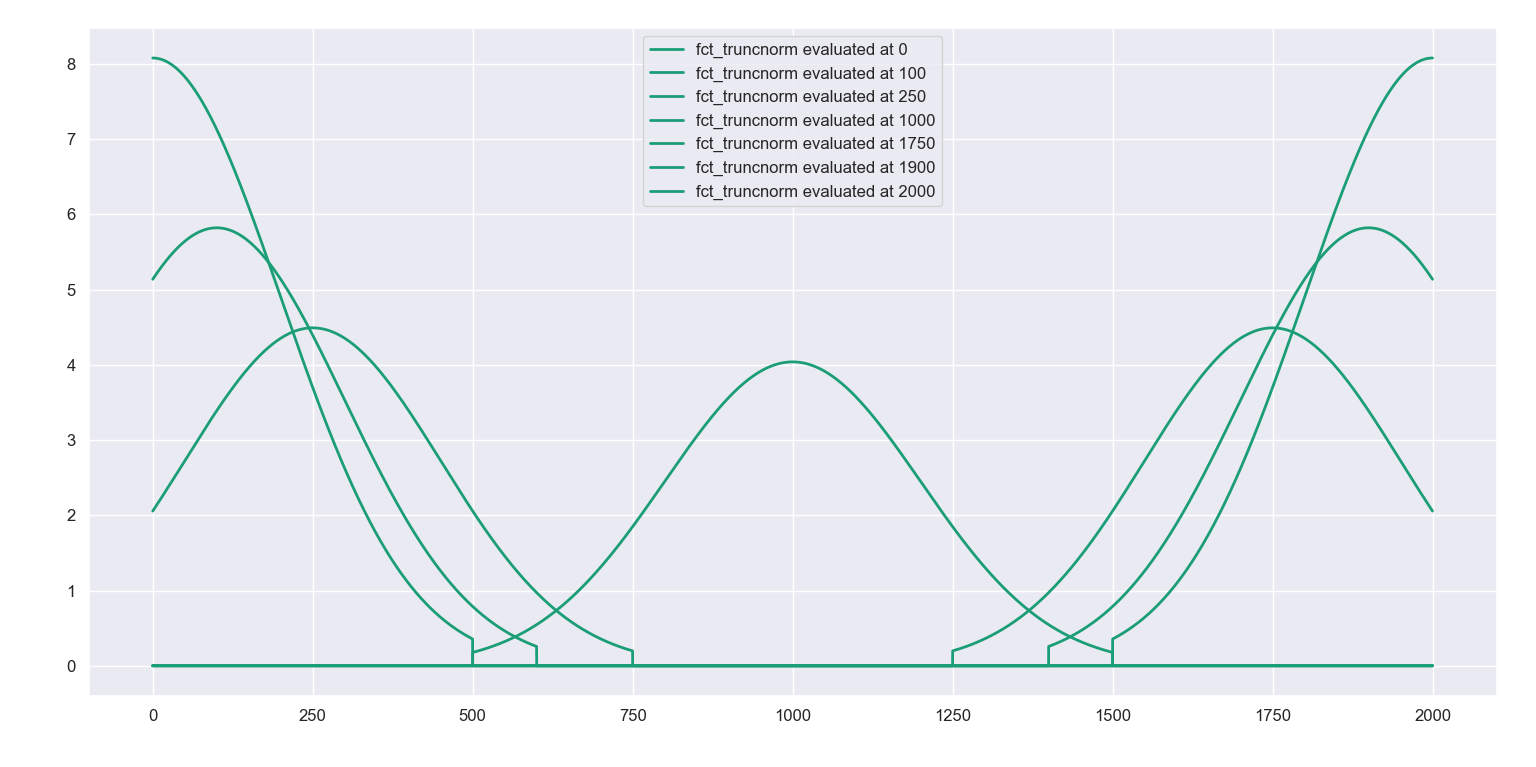
\includegraphics[width = 0.99 \textwidth]{../imag/chap2/impact_edge_kernel.png}
\caption{Shape of the kernel, depending on where it is located on the interval $[0,T]$; here $T = 2000$.}
\label{fig:scaling_kernels}
\end{figure}



\section{Sum-Up Algorithms}
\subsection{Algorithm for Adaptive WMLE}
Following the algorithm \ref{algo:adaptive1}, we write our final version of the adaptive weighting algorithm. The major changes that we apply are:

\begin{itemize}
\item rescale the weights $t$ instead of the kernels $t_i$, for computational reasons,
\item usage of the norm upon the estimate $\theta^*$\footnote{after rescaling the different coefficients as suggested.},
\item change the rescale function $g$ defined in eq. (\ref{eq:new_g}). The function $g$ is seen as a two-dimensional function; the rest of the parameters are fixed.
\end{itemize}


We then get the new scaling parameters:


\begin{equation}
\forall t \in \sequencetime, \qquad \lambda_{t} :=  
g \left (\norm{\widetilde{\theta_{t}}}_{l^2}, 
G_{\norm{\widetilde{\theta_{\cdot}}}_{l^2}} \right)   
\end{equation}

and  $ G_{\norm{\widetilde{\theta_{\cdot}}}_{l^2}} $ is based upon the sequence $\{ \norm{\widetilde{\theta_{\cdot}}}_{l^2} \} $


The algorithm becomes:


\begin{algorithm}[H]
\label{algo:adaptive2}
\SetAlgoLined
1. \quad Find a pilot estimate coined $\widetilde{\theta_t}$. We use the optimal weight from section \ref{section:FWW}, which for a weight $w^*$ and a bandwidth $h^*$ is of the form  $$ (t, t_i) \to \frac 1 {h^*} w^* \left ( \frac{t_i - t }{h^*} \right ) $$ 

2. \quad $\forall t \in \sequencetime$, when we estimated the pilot estimate $\widetilde{\theta_t}$, create the local width factor $\lambda_t$ according to eq. (\ref{eq:local_width_factor}). 

3. \quad Find the final estimate $\hat{\theta_t}$ by using a different weight for each different time $t$. 

$\forall t \in [0,T]$, the new weight shall be of the form:
$$ (t, t_i) \to \frac 1 {\lambda_{t} h^*} w^* \left ( \frac{t - t_i}{\lambda_{t} h^*} \right )$$ 
\caption{Adaptive Kernel Estimation}
\end{algorithm}








\chapter{Numerical Results}

\section{Presentation}
This section is for presenting some empirical observation from the new introduced function $g$ defined in theorem \ref{thrm:new_g}. We first precise our settings, then the results and we try to give some meaningful observations and interpretations.

\section{Considered Evolution for the Parameters}
\begin{figure}
\centering
\subfloat{{
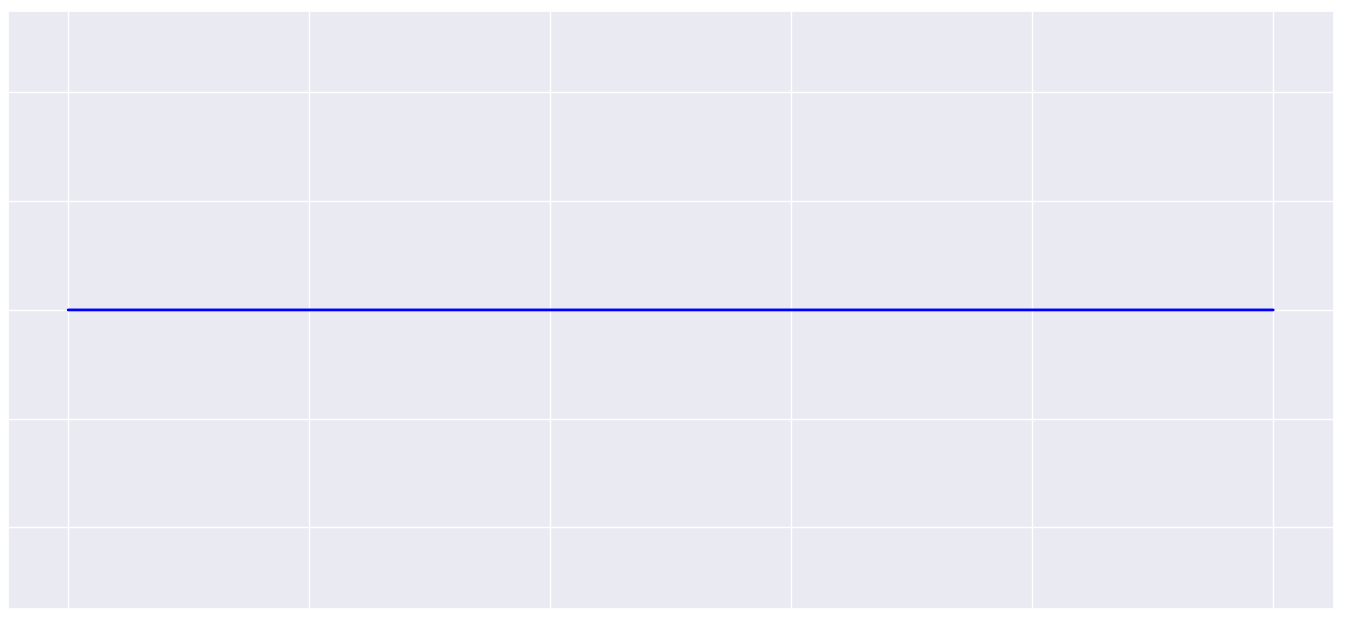
\includegraphics[width = 0.32 \textwidth]{imag/chap3/EVOL_PARAM/Figure_1.png}
}}
\subfloat{{
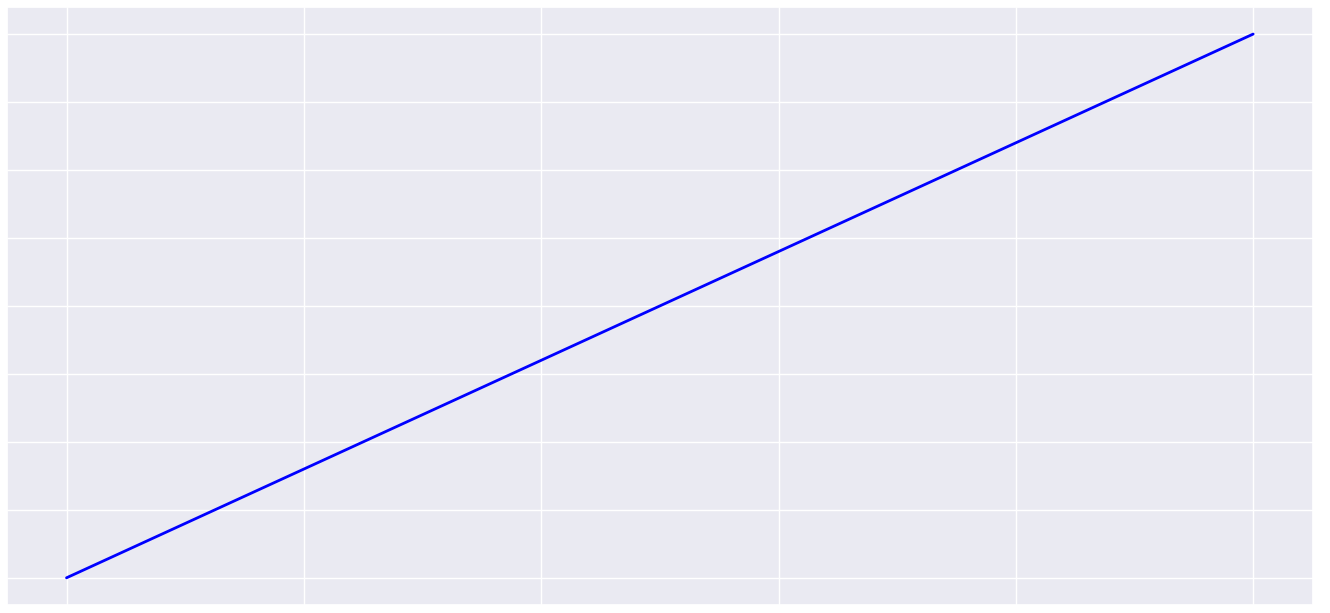
\includegraphics[width = 0.32 \textwidth]{imag/chap3/EVOL_PARAM/Figure_2.png}
}}\\
\subfloat{{
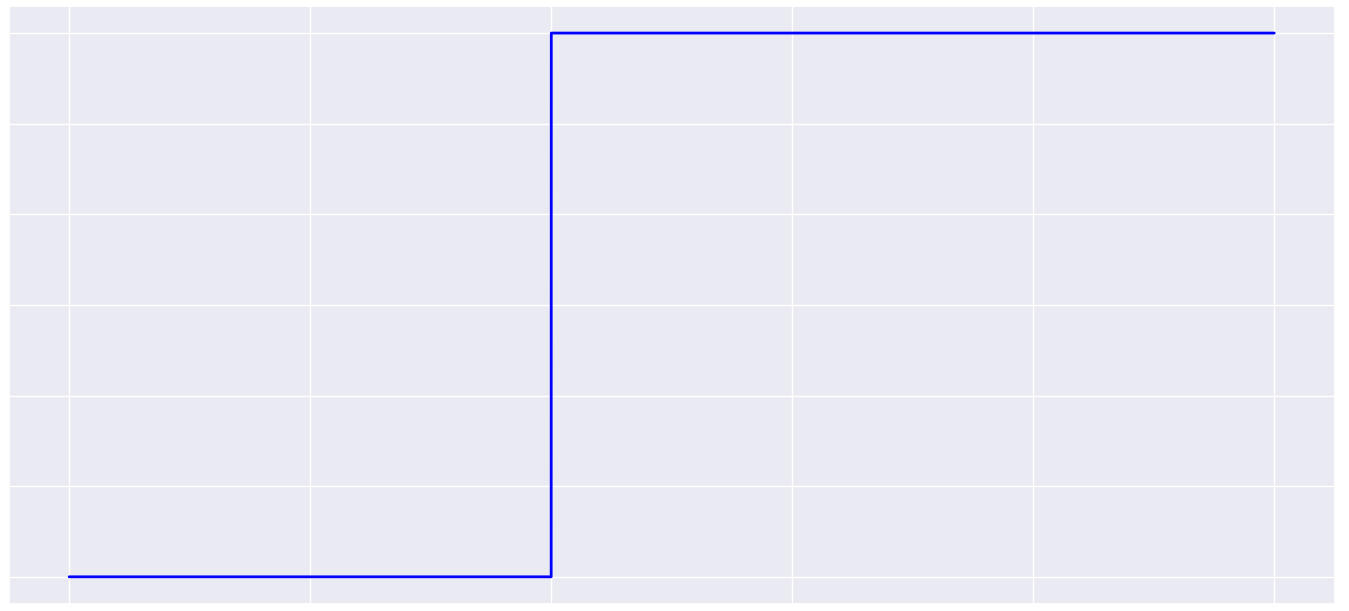
\includegraphics[width = 0.32 \textwidth]{imag/chap3/EVOL_PARAM/Figure_3.png}
}} 
\subfloat{{
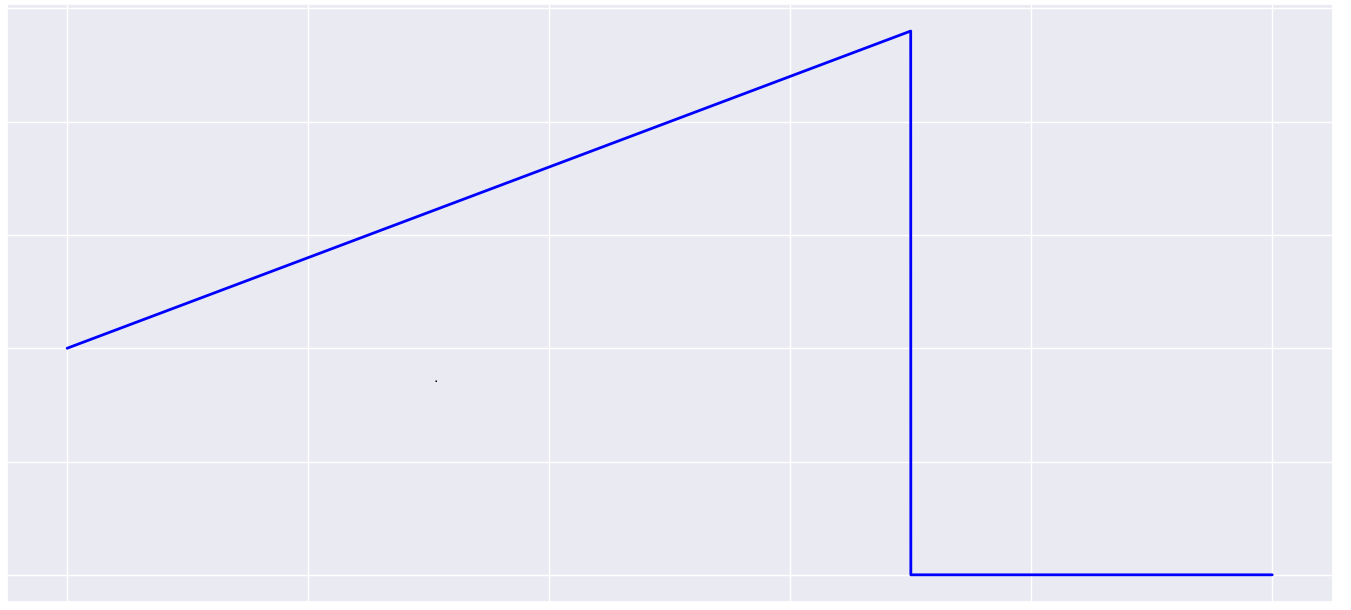
\includegraphics[width = 0.32 \textwidth]{imag/chap3/EVOL_PARAM/Figure_4.png}
}}\\
\subfloat{{
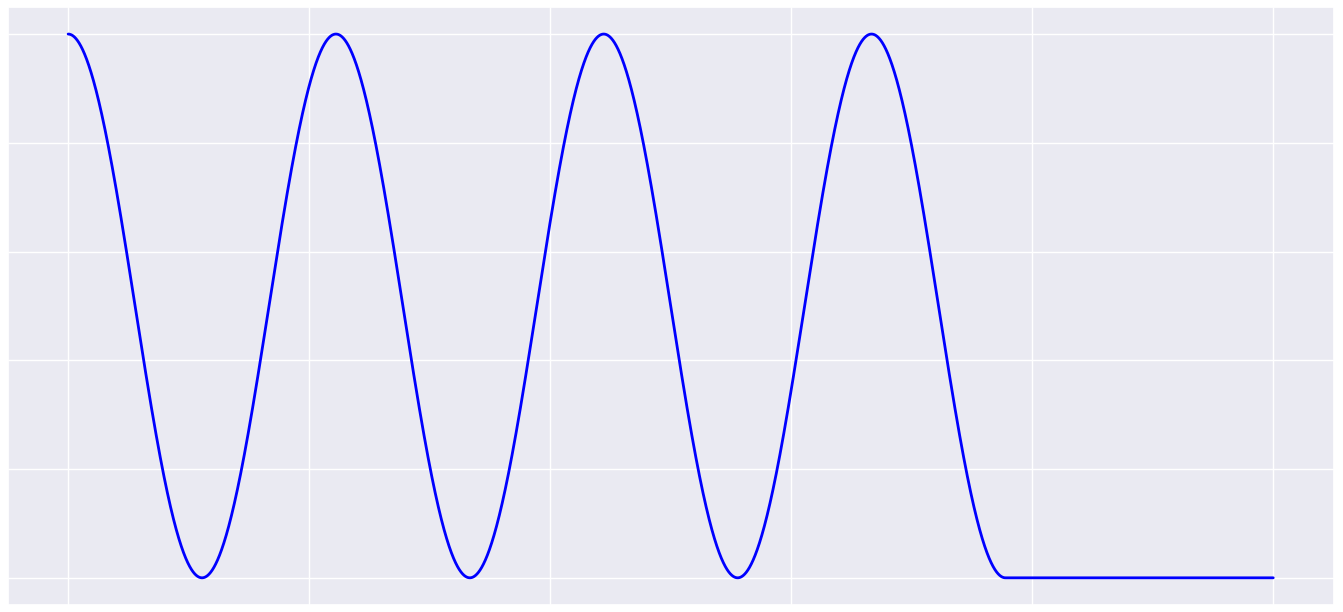
\includegraphics[width = 0.32 \textwidth]{imag/chap3/EVOL_PARAM/Figure_5.png}
}}
\caption{Plots of the different evolutions we consider.}
\label{fig:evol_functions}
\end{figure}

We are going to consider a few evolution functions for the parameters. We want to see how different functions influences the results. We chose constant parameters, linear evolution, one-jump evolution (piece-wise constant), linear evolution combined with one-jump evolution and finally a sinusoidal evolution followed by a constant value. In the three last, there is a breakpoint in the function: either a jump, or the stop of a periodic behaviour. This choice is motivated for change-point analysis in 
chapter \ref{chap:change_point}. We observe the basic functions in figure \ref{fig:evol_functions}.

Essentially, in the univariate case, we plot in fig. \ref{fig:evol_functions_interact} how the parameters evolve with respect to each other. Those coefficients are the one we use for the simulations. 

\begin{figure}
\centering
\subfloat{{
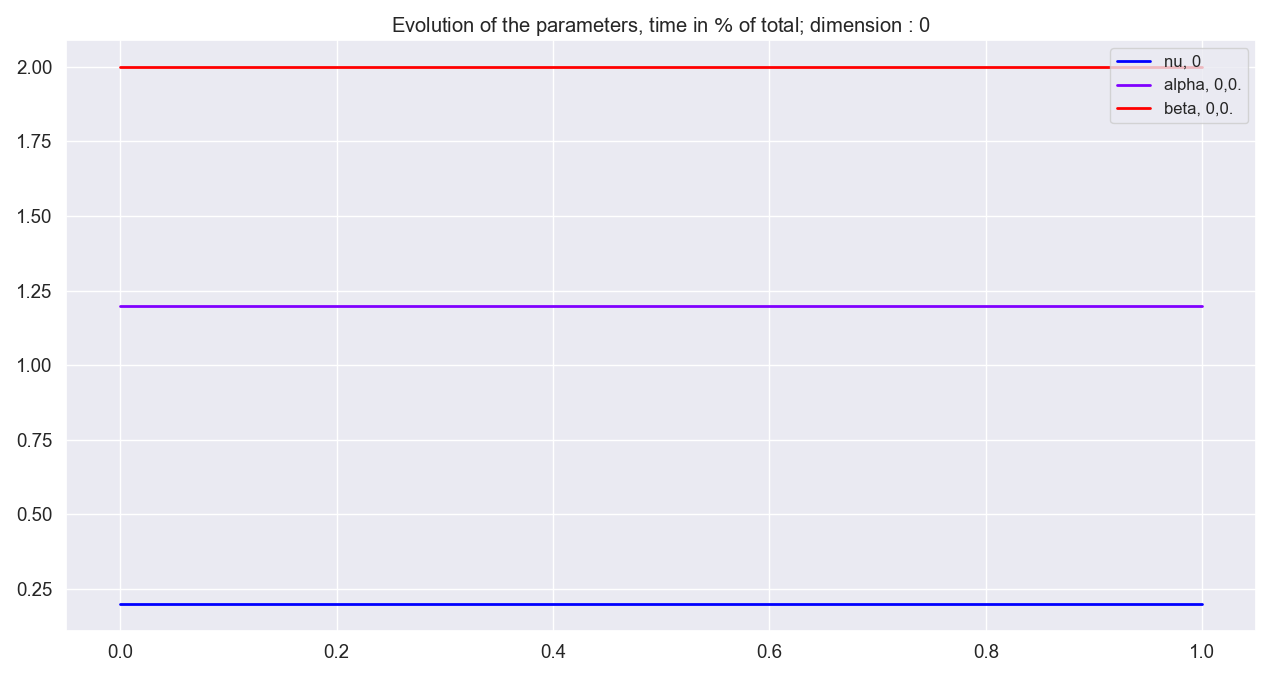
\includegraphics[width = 0.48 \textwidth]{imag/chap3/EVOL_PARAM/AFigure_1.png}
}}
\subfloat{{
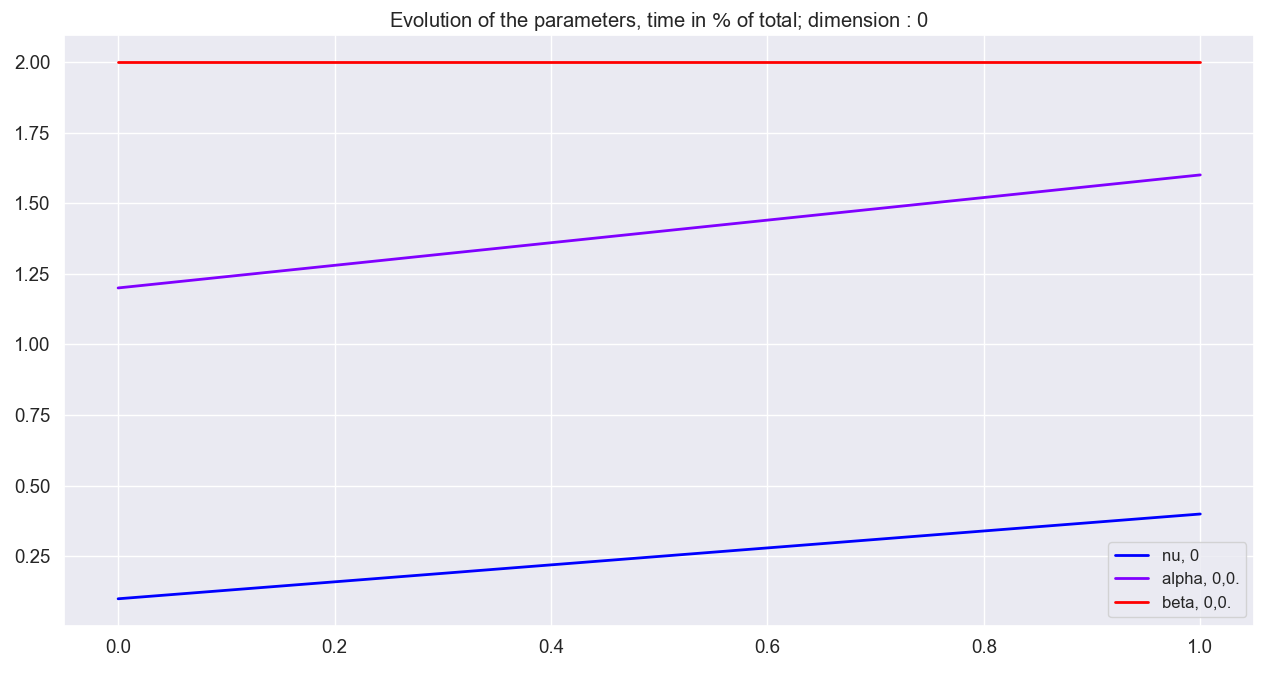
\includegraphics[width = 0.48 \textwidth]{imag/chap3/EVOL_PARAM/AFigure_2.png}
}}\\
\subfloat{{
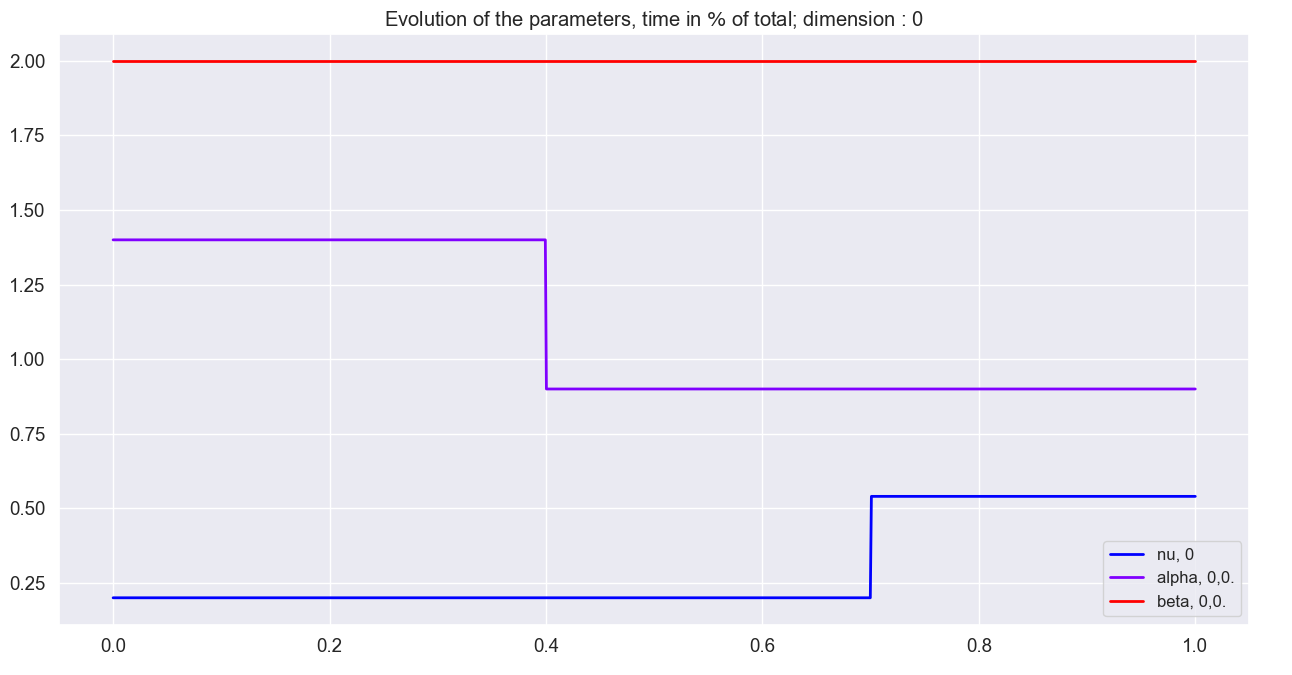
\includegraphics[width = 0.48 \textwidth]{imag/chap3/EVOL_PARAM/AFigure_3.png}
}} 
\subfloat{{
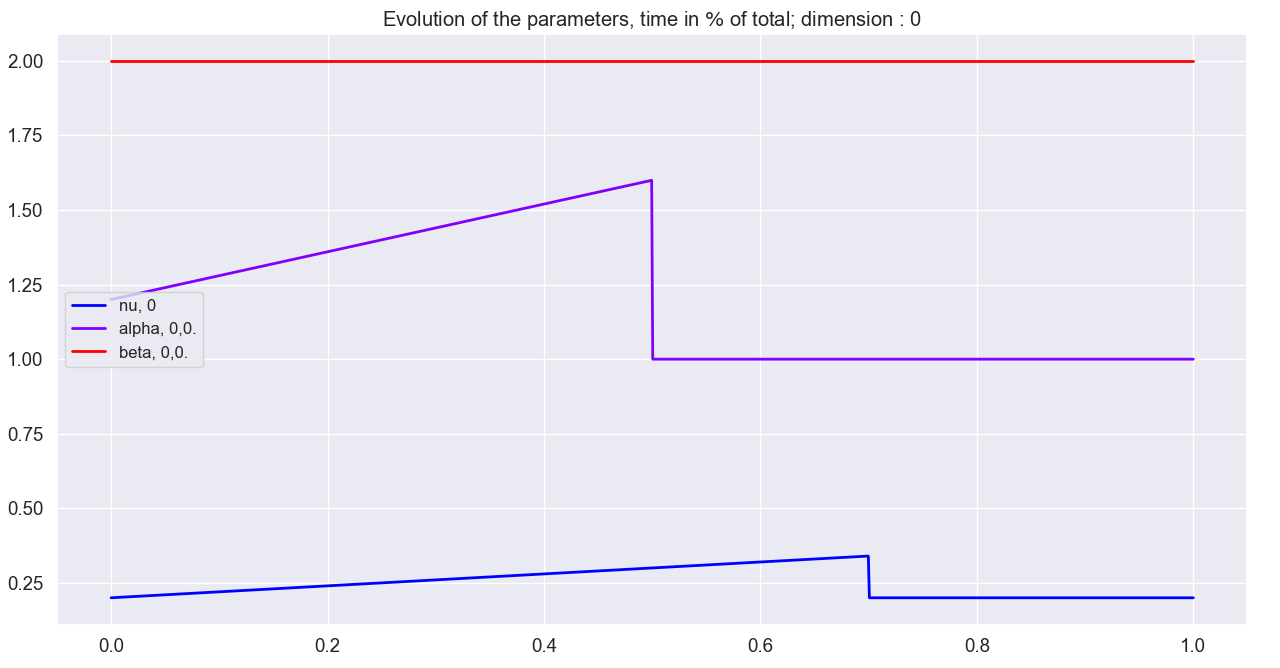
\includegraphics[width = 0.48 \textwidth]{imag/chap3/EVOL_PARAM/AFigure_4.png}
}}\\
\subfloat{{
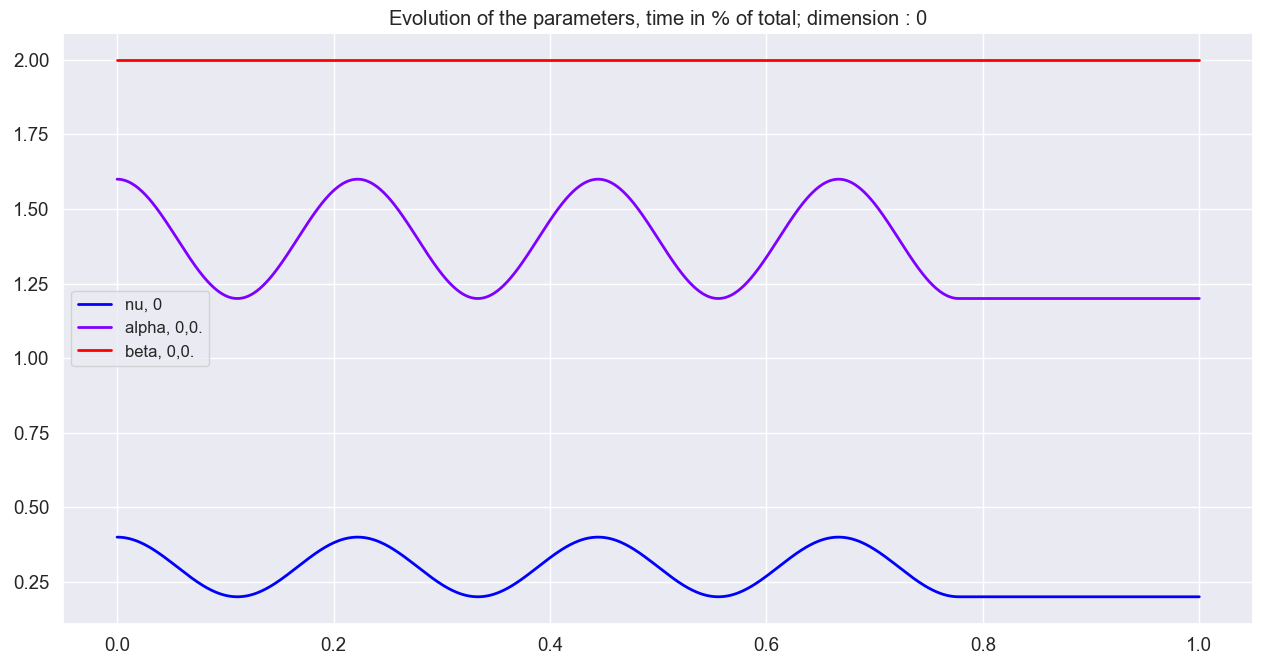
\includegraphics[width = 0.55 \textwidth]{imag/chap3/EVOL_PARAM/AFigure_5.png}
}}
\caption{Plots of the three parameters of a Hawkes process. Red is $\beta$, purple is $\alpha$ and the blue line represents the evolution of $\nu$. The 5 shapes are the one we consider and are related to the functions ploted on fig. \ref{fig:evol_functions}.}
\label{fig:evol_functions_interact}
\end{figure}













\section{Naïve Estimation}
As a first array of trials, we consider our recommanded parameters: $L$ and $R$ defined respectively as being the $2$ and $98$ quantiles; $h$ and $l$ being respectively $2.5$ and $0.2$. 

We are also going to use $1/5$ of the total observation length as being the width for the kernels of the first estimate, following the recommandation from section \ref{subsection:optimal_width}. 

\subsection{Constant parameters}
The figures are drawn in apendix as: \ref{fig:first_estimate_0_alpha}, \ref{fig:first_estimate_0_beta}, \ref{fig:first_estimate_0_nu}. 


We previously mentionned how the scaling is interfering with rescaling the kernels for constant parameters. The scaling is then more focused on the noise than anything relevant about the data (cf subsection \ref{subsection:scaling}). We draw on the fig. \ref{fig:impact_g_flat} some estimation for one parameter (based on the same data as for \ref{fig:first_estimate_0_nu}), and we observe how it impacts the kernel adaptive process. The evolution is hectic and there is definetely no clear pattern. In such case, one should increase the width of the kernels to the maximum and weight all the data in the same manner. Basically, the first estimate parametrize the second as being a constant estimation. 

\begin{figure}
\centering
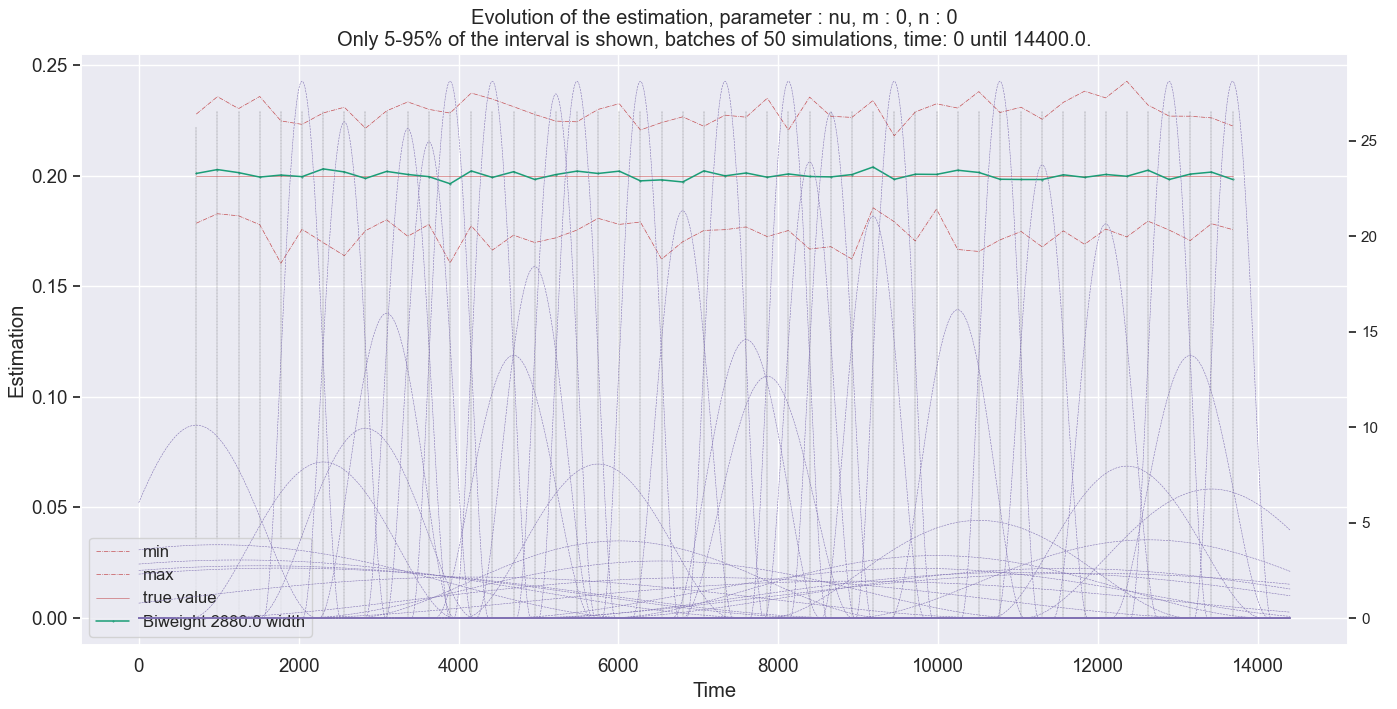
\includegraphics[width = 0.90 \textwidth]{../imag/chap3/IMPACT_G/flat_all_kernels.png}
\caption{TO WRITE.}
\label{fig:impact_g_flat}
\end{figure}

The second step's plots is displayed with fig. \ref{fig:second_estimate_0_alpha}, \ref{fig:second_estimate_0_beta}, \ref{fig:second_estimate_0_nu}

We observe an expected improvement. It isn't directly induced by $g$, but by the scaling tolerance we introduced. It deals very well with such trends.

\subsection{Linear growth}
The figures are drawn in apendix as: \ref{fig:first_estimate_1_alpha}, \ref{fig:first_estimate_1_beta}, \ref{fig:first_estimate_1_nu}.

Let's first give a look to how the kernels are evolving with the first estimate. On fig. \ref{fig:impact_g_linear}, we see the expected behaviour for the evolution of the kernels. Extreme values are estimated with smaller kernels, and values close to the mean with wider kernels\footnote{They are wide and it makes sense. Both sides compensate each other, the parameters in the middle appear like being the average of the whole observed period.}. At the core, it is the behaviour one could expect.

\begin{figure}
\centering
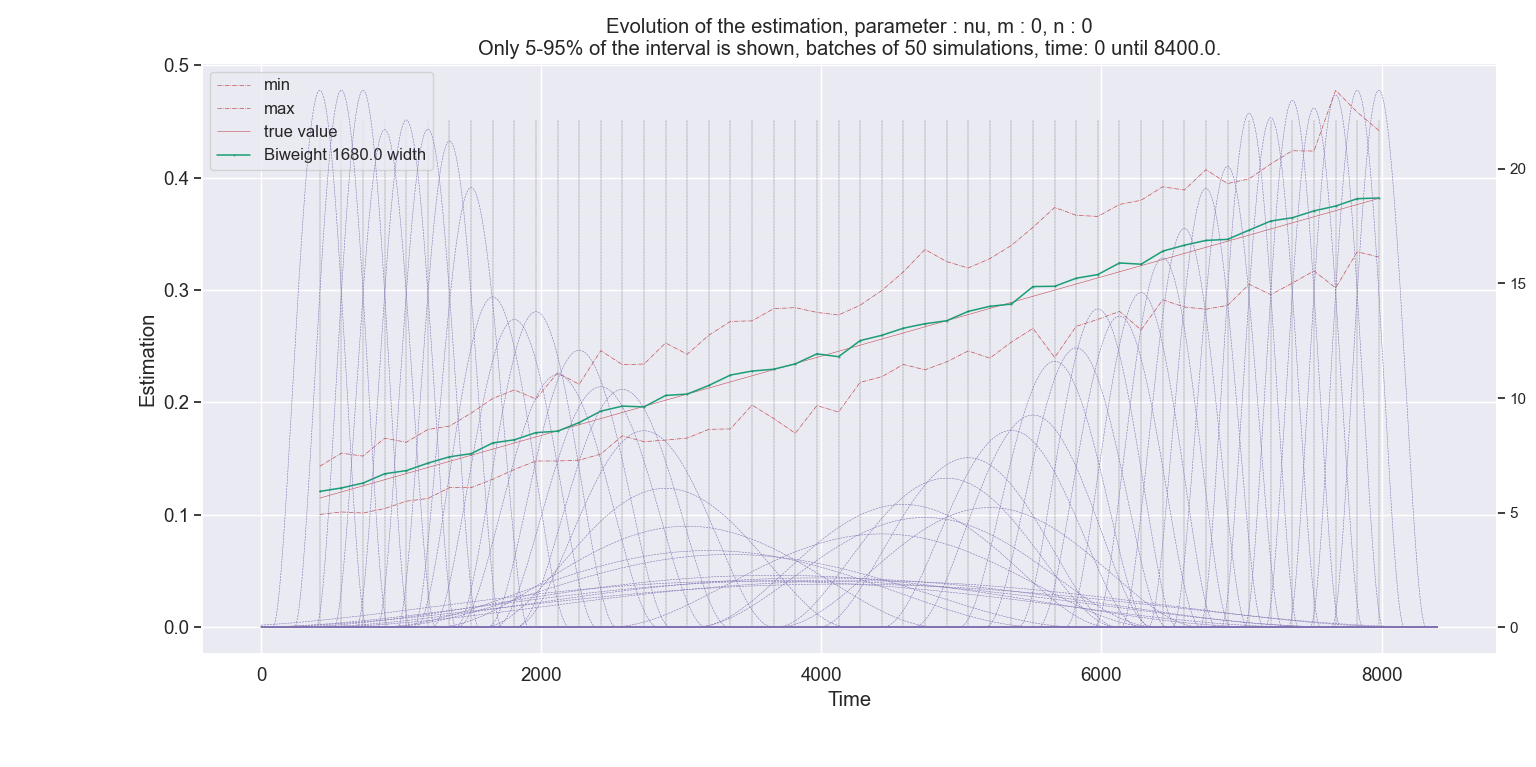
\includegraphics[width = 0.90 \textwidth]{../imag/chap3/IMPACT_G/linear_growth_all_kernels.png}
\caption{TO WRITE.}
\label{fig:impact_g_linear}
\end{figure}


The second step's plots is displayed with fig. \ref{fig:second_estimate_1_alpha}, \ref{fig:second_estimate_1_beta}, \ref{fig:second_estimate_1_nu}. It does show some improvements, since the estimate looks overall flatter. Then, the function $g$ works great for linear trends. The points where the kernels are the smallest show signs of more variability. This is due to having a parameter $h$ too big.







\subsection{Simple jump}
\willdo{to simulate and write}

The figures are drawn in apendix as: \ref{fig:first_estimate_2_alpha}, \ref{fig:first_estimate_2_beta}, \ref{fig:first_estimate_2_nu}.

The second step's plots is displayed with fig. \ref{fig:second_estimate_2_alpha}, \ref{fig:second_estimate_2_beta}, \ref{fig:second_estimate_2_nu}.

\begin{figure}
\centering
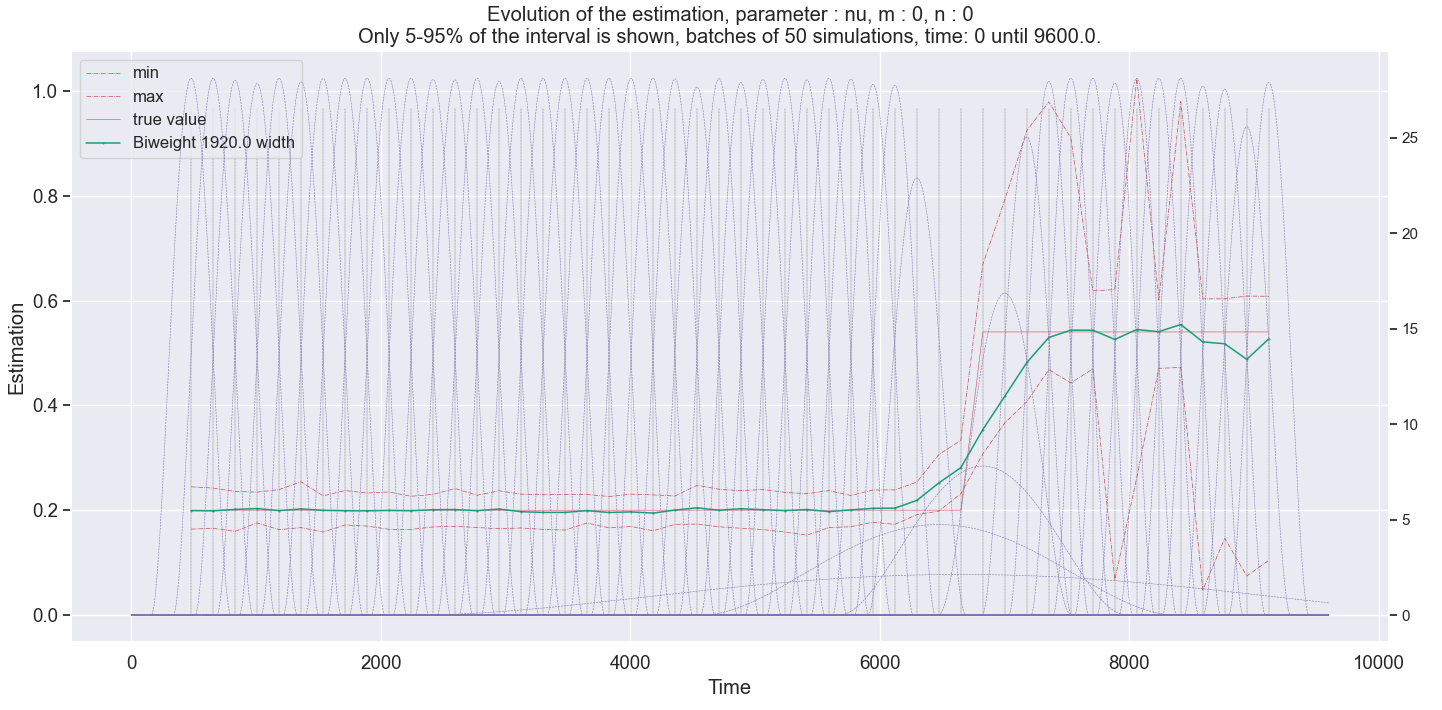
\includegraphics[width = 0.90 \textwidth]{../imag/chap3/IMPACT_G/jump_all_kernels.png}
\caption{TO WRITE.}
\label{fig:impact_g_jump}
\end{figure}



\subsection{Linear growth and jump}
\willdo{to simulate and write}
The figures are drawn in apendix as: \ref{fig:first_estimate_3_alpha}, \ref{fig:first_estimate_3_beta}, \ref{fig:first_estimate_3_nu}.

The first estimate struggle to capture accuratly the jump. There is a transition phase between the two behaviours that could be improved. For parameter $\alpha$, it last for 1000, for parameter $\nu$ roughly 800. It corresponds to the size of the kernel.

The second step's plots is displayed with fig. fig. \ref{fig:second_estimate_3_alpha}, \ref{fig:second_estimate_3_beta}, \ref{fig:second_estimate_3_nu}.

We see that the jump is way better estimated. The transition i








\begin{itemize}
\item the jump was estimated very smoothly. And the transition isn't very clear, for alpha the estimate lowers roughly around the jump while for parameter nu, it lowers way before the jump.
\item the adaptive improves how accurate the jump is noticeable for alpha as well as for nu. For alpha, the jump is sharper at left, and for nu sharper on the right. This is due to the dimensionality of the problem. Since the same kernels are used for all parameters' estimation, it is complicated to fit the perfect size at all times when different parameters need different kernels. Overall, the two jumps are better localized, and the function is sharper, though it was not intended for that aim. 
\item This comes at the price of having slightly less precise estimates elsewhere, mainly because the kernels are narrower, but also we notice an interesting phenomena: for the estimate of alpha for example, the first estimates are over-estimating the true value. This is due to the fact that the kernel is bigger (since the value is close to the geometric mean), but though the geometric mean is computed over the whole observation window, the kernel is only taking into account part of it. 
\item We observe here that the value $l$, parameter of $g$ should actually be smaller than the ratio used for the width. That way, the kernel would consider more data.
\end{itemize}

\subsection{Sinusoïdal growth}
\willdo{to simulate and write}
The figures are drawn in apendix as: \ref{fig:first_estimate_4_alpha}, \ref{fig:first_estimate_4_beta}, \ref{fig:first_estimate_4_nu}.

The second step's plots is displayed with fig. \ref{fig:second_estimate_4_alpha}, \ref{fig:second_estimate_4_beta}, \ref{fig:second_estimate_4_nu}.

\begin{itemize}
\item changing point better captured
\item rupture between behaviours seems to be noticed by $g$ and behaves differently on both sides.
\item the ups are way more accurate, though the the downs are smoothed (by wide kernels). It seems that since the first estimate wasn't able to capture precisely the low part, the function $g$ smoothed out that behaviour even more. The solution we will try is to put smaller kernels from the beginning.
\item Also, the function is way less smooth. Before, one could definetely recognise a sinus function, though shifted. Now, it has some weird spikes at some points. We do believe it is because of the too wide first kernels.
\end{itemize}

\begin{figure}
\centering
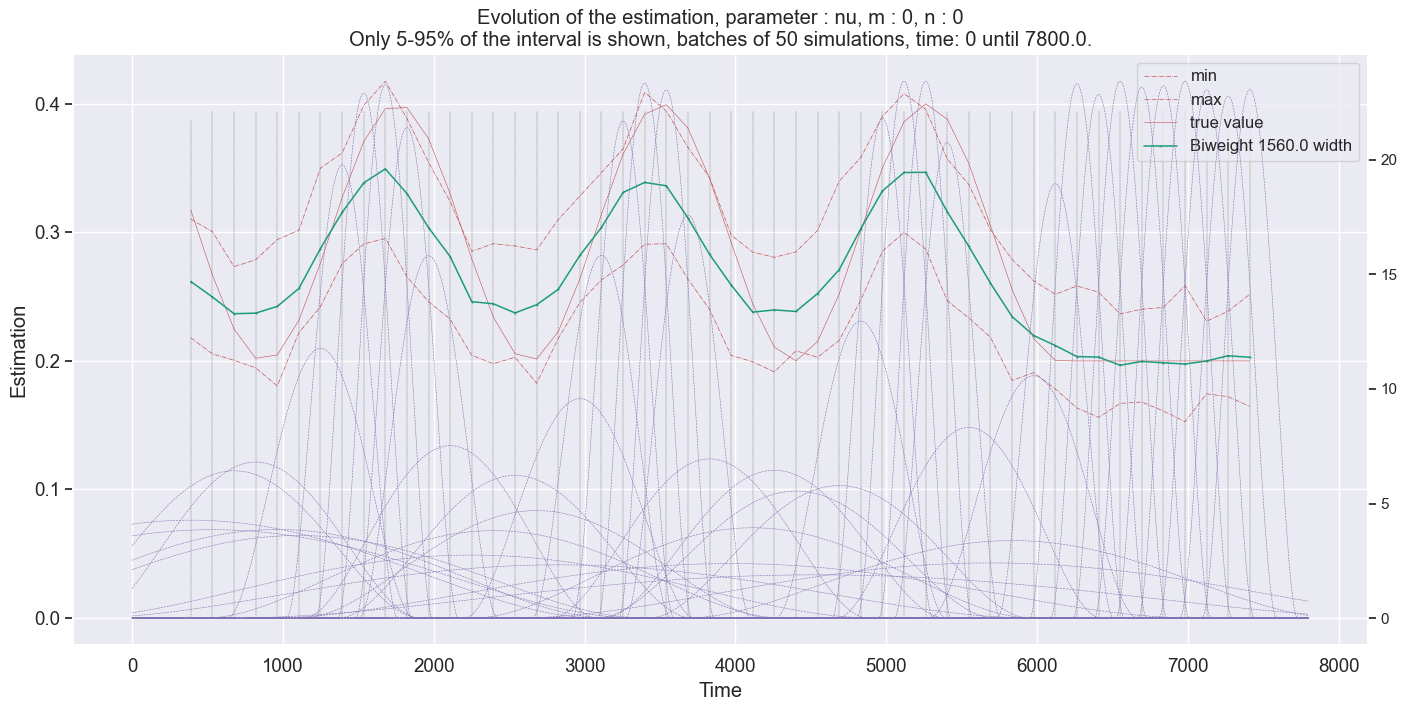
\includegraphics[width = 0.90 \textwidth]{../imag/chap3/IMPACT_G/sin_all_kernels.png}
\caption{TO WRITE.}
\label{fig:impact_g_sin}
\end{figure}




\section{Second approach}
We learnt that the first width is crucial in the result of the second estimate. We also learnt that depending on the first width, $l$ should change. 







\section{Exploration of Adjustable Parameters}
\label{section:exploration}


I don't know about this...
































\section{Other Fancy Methods}
\subsection{Radial Basis Function}

I won't have time for that. There was the topic of radial basis function as well as the truncated kernels I saw in Wand. 


\willmuchlater{Need to read about method. \newline and write about it. \newline. Perhaps I wont have the time.}

\willmuchlater{ I also want to look at the truncated kernels. Notamment, sait-on si il y a un jump ou non?}






\chapter{Change Point Analysis}
\label{chap:change_point}

We are going to study the functions from \ref{fig:evol_functions}.

PACKAGE RUPTURE.



\willmuchlater{write chapter about change point analysis.}











































\cleardoublepage% le corps du document est terminé

\appendix
\pagestyle{back}




\part{Appendix}
\chapter{Background of methods in order to simulate Hawkes Processes}
\label{appendix_simulate}


\section{Methods for simulating a Hawkes Process}
\label{section:definition_algo}
We describe a few algorithms for simulating Hawkes processes. We will give a particular attention to the following criteria:

\begin{itemize}
\setlength{\itemindent}{2 cm}
\item Exact (without resorting to approximation)
We refer to subsection \ref{subsection:edge} for more details about edge effect. One also defines exact as a method of drawing an unbiased associated estimator throughout the entire simulation process. \willprecise{Not sure about the meaning of exact. It would have to be checked.}
\item Efficient (no wastage, not using the rejection sampling)

\begin{definition}[Rejection Sampling]
Rejection Sampling is a basic technique used to generate observations from a distribution. One uses another distribution on a wider set $\mathcal Y$ in order to simulate values inside $\mathcal X \subset \mathcal Y$. A classic example is using a uniform distribution over a rectangle in order to create one on a circle, by rejecting all points outside the circle. 
\end{definition}

An algorithm that uses rejection sampling method is called non-efficient. 

\item Flexible (all parameters in $\Theta$ as defined previously: $ \Theta = ( \nu, \alpha, \beta ) $ )
\item Followable (source triggering the event is known)
\item Perfect (take past history into account, i.e. no "edge effect")
\item Markable (jumps can be marked; marked Hawkes process)
\item Multivariate (the algorithm supports multi-variate Hawkes process)
The criteria flexible and followable do make sense if and only if the multivariate version of the algorithm is available.
\end{itemize}


By the fact that a Hawkes process can be seen either as a non-homogeneous Poisson process or a branching process, there exists two essentials classes of simulating methods respectively: intensity based and cluster-based simulation. Intensity based methods have been studied for a long time, and many methods exists. We are going to talk about the ones that have been applied and consensual accepted in the literature. They gather into three categories: inversion, order-statistics methods and rejection sampling. We refer to \cite{gen_nonhomo_poisson} for a detailed description of the categories (a dozen algorithms are also proposed).



\subsection{Intensity based simulation}
\label{subsection:thinning}
Hawkes process generation can be viewed as the simulation of an inhomogeneous Poisson process. Indeed, the intensity is globally random, with deterministic segments in between jumps ( $\forall k \in \N, ]t_k, t_{k+1}]$ is a deterministic segment). For that reason, one can use the classic thinning algorithm (also referred to as the Lewis-Shedler thinning algorithm) whose pseudo-code can be found in \cite{lewis} and whose simplest version is well described in \cite{socialhawkes} eq. (1.18). 

Lewis' algorithm works well enough in the settings of fixed intensity functions, its main drawback is the need for a bound on the intensity that holds over an interval for all histories of the process. This, is a tremendeous flaw for applications to processes with random conditional intensities (as Hawkes processes). This difficulty has been overcomed with Ogata, whose algorithm requires only a local boundedness condition on the conditional intensity.
It is readable in \cite{Ogata} (the so called Ogata's modified thinning algorithm). 


A clear sum-up is available at the end of \cite{simullaub}. One can also find a very clear and detailed review of intensity-based algorithms in \cite{daley}, section 7.5. In particular, they mention in algorithm 7.5.II. the Lewis algorithm; algorithm 7.5.IV the Ogata's polishing and at 7.5.V. the thinning algorithm for marked point processes. 

Thinning methods fall into the category of Acceptance-Rejection methods and are not described as efficient for the reason that for $N$ events, they usually impose a complexity of $o(N^2)$. This is due to the rejection sampling method they rely on.


We write down one version of a thinning algorithm, which, as explained allows to simulate any non-homogeneous Poisson process, by knowing its deterministic intensity function:

\begin{algorithm}[H]
\label{algo:thinning_algo}
\SetAlgoLined
$t_0 = 0$,

$r_0 = 0$,

$j = 0$ and $i = 0$,

$\overline{ \lambda } = \sup_t \lambda( t ) $,

\While {$r_j < T$}
				{Sample $u \sim \text{uniform}(0,1)$, 
				
				Sample $a \sim \exp( \overline{ \lambda } )$,
				
				Set $r_{j+1} = r_j + a$,
				
				D $\sim \text{uniform}(0,1)$,
				
				\If{$ D \leq \lambda( r_{j+1} ) / \overline{\lambda} $ }
					{$t_{i+1} = r_{j+1}$,
				
					$i = i+1$,
					}
				$j = j+1$,
				}
\eIf{ $t_i \leq T$}{ return $\{t_k\}_{k = 1, \cdots, i}$. }
{ return $\{t_k\}_{k = 1, \cdots, i-1}$. }


\caption{Thinning algorithm for non-homogeneous Poisson process.}
\end{algorithm}

\begin{remarque}
Notice that instead of the condition:

\begin{align*}
D & \sim \text{uniform}(0,1) \\
\text{if } & D \leq \frac {\lambda( r_{j+1} ) } { \overline{\lambda} } 
\end{align*}


one could use equivalently:

\begin{align*}
D & \sim \text{uniform}(0, \overline{\lambda}) \\
\text{if } & D \leq \lambda( r_{j+1} ) 
\end{align*}


\end{remarque}


\begin{remarque}
Thinning algorithm relies on the idea of supremum for the intensity. For that reason, as noticed in \cite{daley}, a condition for applying such algorithm is that 

"there exists functions $M(t \mid \mathcal F_{t^-} )$ and $L(t \mid \mathcal F_{t^-} )$, such that $\forall t \in [0, \infty [$ and all list-history, the conditional intensity functions $\lambda$ of the process satisfy:

$$ 0 \leq u < L(t \mid \mathcal F_{t^-} ), \qquad  \lambda( t + u  \mid \mathcal F_{t^-} )  \leq M( t \mid \mathcal F_{t^-} )  $$

Then for any marked simple point process, the difficulty is reduced to find such functions $M,L$."


\end{remarque}

\subsection{Superposition based simulation}
Another interesting method for simulating Poisson processes is based upon the immigration-birth representation. The idea is to first simulate the immigrants as a Poisson process. Conditional on the number of immigrants, the time at which the immigrants appear is an order statistics, identically and independently uniformly distributed over the segment\footnote{One can find a proof of that in Cox-Lewis 1962, and quoted in \cite{gen_nonhomo_poisson} as theorem 2.}. The descendants then form an inhomogeneous Poisson process, which can be simulated thanks to another trick. Since we know that the branching representation of the Hawkes process has $\alpha / \beta $ births in average, we simulate the number of descendant with a Poisson law with parameter $\alpha / \beta$ and then add the new jumps by computing the inter-arrival time, immigrant-son, of an homogeneous Poisson process with parameter $\beta$.

The algorithm can be found in \cite{simullaub}. We would like however, to point-out that the algorithm is incomplete. The algorithm generates the immigrants as well as the first generation of the offspring and then stops. What should be added is a for-loop on the next generations until no new offspring is generated.




\subsection{Other Used Methods in the Literrature}
We highlight the algorithm proposed by Møller and Rasmussen \cite{rasmussen}, which is a perfect method in the sense of our definition at the beginning of the section.

An interesting evolution of thinning has been given in \cite{simuldassios}, where the authors are using superposition as well as thinning in order to reduce the complexity of the algorithm. The methods are vulgarized in \cite{socialhawkes} eq. (1.19). Basically, the authors used the Markov property of Hawkes process (granted by the exponential kernel). They also include in the algorithm the possibility of having a different starting intensity than the asymptotic underlying intensity (as previously mentioned in section \ref{section:dassios}. 

\willprecise{ exponential kernel implies markov. Mettre une référence à une section ou j'en parle mieux?}


The biggest flaw of that algorithm is that in the multivariate case, all the decays need to be identical. There is however, another algorithm that generalize \cite{simuldassios}'s one (in the sense they are also using thinning and superposition) but they did manage to get the desired flexibility. The algorithm is very well stated inside \cite{my_algo_simul}. Also, usually only cluster-based algorithm conveys information regarding the source that triggers the event times. For that reason, \cite{my_algo_simul} is an interesting algorithm on the innovative perspective.



All the previously mentioned algorithm are summed-up in the table \ref{table:methods_HP}.


\section{Pitfalls of Simulation}
\subsection{Burn-In}
\label{subsection:burn}
We want to simulate Hawkes processes over finite time windows. Unfortunately, the described methods are partially failing, as the past of the process is not known and cannot be simulated, at least not completely.

Burn-in period: for non-exact methods, a burn-in period shall be introduced to the process in order for it to reach a stationary state. Then, the effects of any transients from the initial conditions become negligible. Finding the optimal length of such period is an important question that we have not delved into.


For the sake of demonstration, we show in fig. \ref{fig:burn-in} how the burn-in impacts the process. One sees that the intensity at the beginning of the process becomes random. It is important to not include the burn-in period inside the data used for estimation. 

\begin{remarque}
Skipping the burn-in period is never recommended, though the results between the estimation given either by processes including a burn-in period or without weren't different in any significative manner.
\end{remarque}

In particular, for time-dependent parameters, the burn-in period doesn't seem to be sufficient. It was intended for reaching stationarity, though the process isn't. For that reason, in the case of time-dependent parameters, one should not change the process' parameters too quickly, or otherwise the simulation might lead to false results.

\begin{figure}
\centering
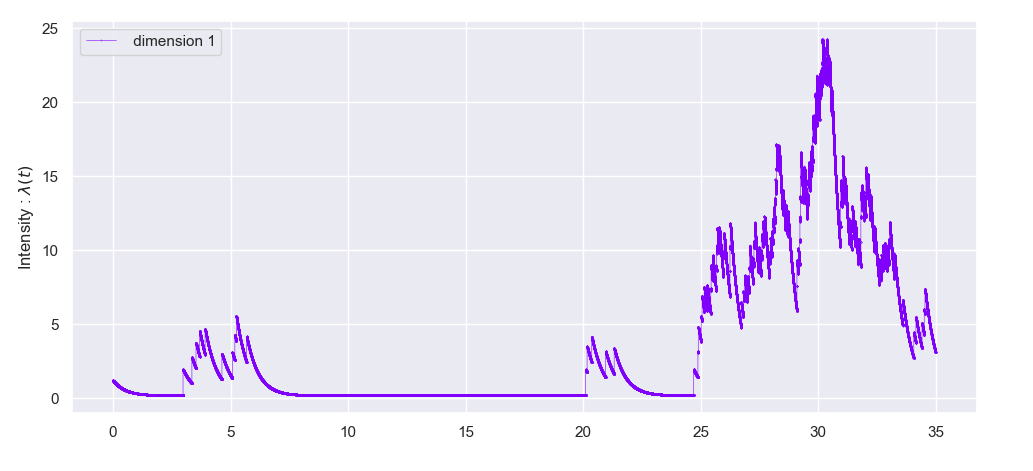
\includegraphics[width = 0.99 \textwidth]{../imag/burnin.png}
\caption{Univariate Hawkes Process with burn-in. One notices the tail of an unobserved event at the beginning of the intensity.}
\label{fig:burn-in}
\end{figure}









\begin{sidewaystable}
\begin{center}
\begin{tabular}{  | m{3.8 cm} || m{1.5 cm} |  >{\centering}m{1.7 cm}  
|| >{\centering}m{1.2 cm}  | >{\centering}m{1.52 cm}  |  >{\centering}m{1.25 cm}  |  >{\centering}m{1.6 cm}  |   >{\centering}m{2.1 cm} |  >{\centering}m{1.4 cm}  | >{\centering\arraybackslash} m{1.8 cm} | } 
\hline
Name of the Method  & Type & Author 
& Exact & Efficient 
& Perfect &  Markable & Multivariate  & Flexible & Followable  \\ 
\hline
\hline
Ozaki's Algorithm & Intensity & \cite{Ozaki} 
& $\times$ & $\checkmark$ 
& $\times$ & $\times$ & $\times$ & $-$ & $-$  \\
\hline
Thinning Algorithm & Intensity &  \cite{lewis}, \cite{simulchen}
& \checkmark & $\times $ 
& $\times$ & $\times$ & $\times$ & $-$ & $-$ \\
\hline
Ogata's Modified Thinning Algorithm & Intensity &\cite{Ogata}, \cite{simulchen}, \cite{multihawkes}
& $\checkmark$ & $\times$ 
& $\times$ & $\times$ & $\checkmark$ & \checkmark & $\times$ \\
\hline
Algorithm 7.5. Daley; & Intensity &\cite{daley}
& $\checkmark$ & $\times$ 
& $\times$ & $\checkmark$ & $\times$ & $-$ & $-$ \\
\hline
Perfect simulation & Cluster & \cite{rasmussen} 
& $\checkmark $ & $\checkmark$ 
& $\checkmark$ & $\checkmark $ & $\times$ & $-$ & $-$ \\
\hline
Exact simulation & Mixed & \cite{simuldassios} 
& $\checkmark $ & $\checkmark$ 
& $\times$ & $\checkmark $ & $\checkmark$  & $\times$ & $\times$\\
\hline
Laub's Cluster algorithm & Cluster &\cite{simullaub} 
& $\checkmark $ & $\checkmark$ 
& $\times$ & $\times$ & $\times$ & $-$ & $-$ \\
\hline
Superposed exact simulation
& Mixed & \cite{my_algo_simul} 
& $\checkmark $ & $\checkmark$ 
& $\times$ & $\checkmark $ & $\checkmark$ & $\checkmark$ & $\checkmark$ \\
\hline
\end{tabular}
\caption{Overview of a few different methods for Hawkes process simulation.}
\label{table:methods_HP}
\end{center}
\end{sidewaystable}
\chapter{Numerical Analysis: Results of Simulations}


\section{First Attempt of the Adaptive Algorithm}


\willdo{changer le nom du 10. et suivants.}
\begin{figure}
\centering
\subfloat{{
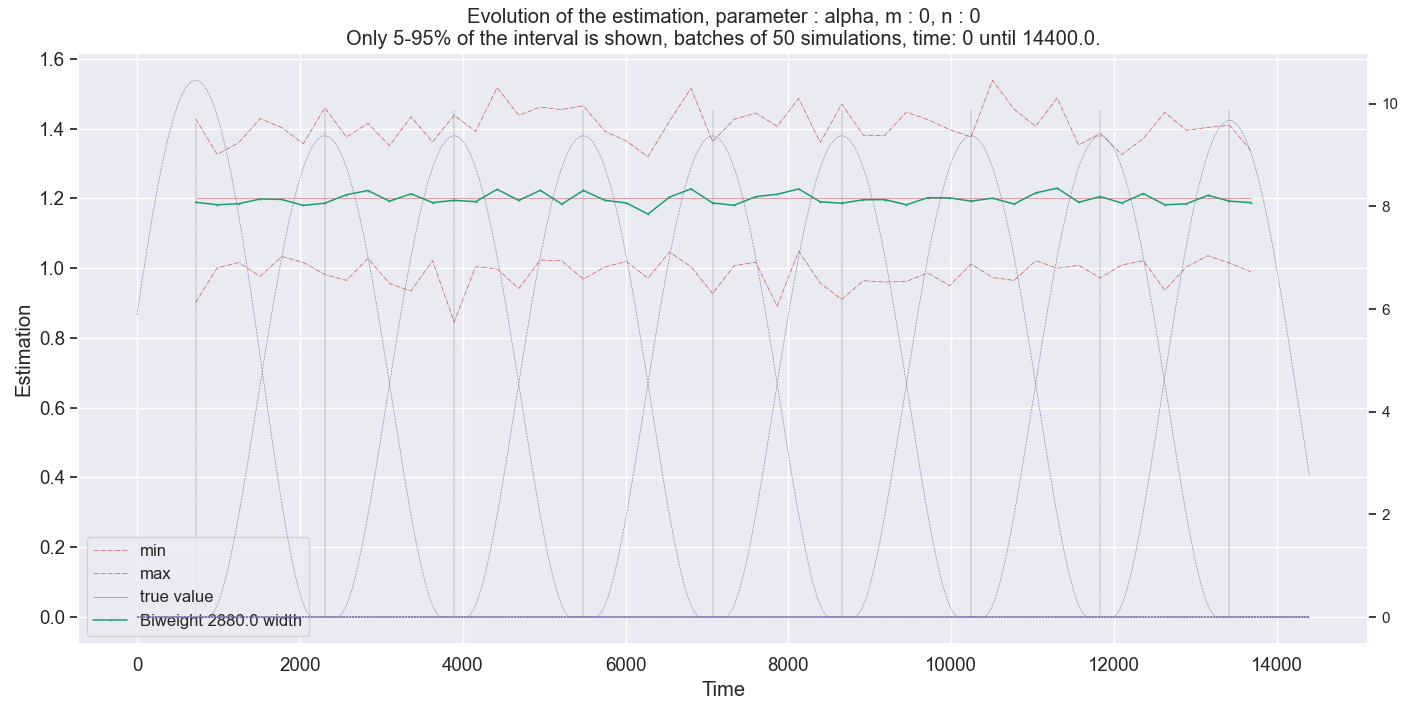
\includegraphics[width = 0.48 \textwidth]{../imag/chap3/0/Figure_2.png}
}} 
\subfloat{{
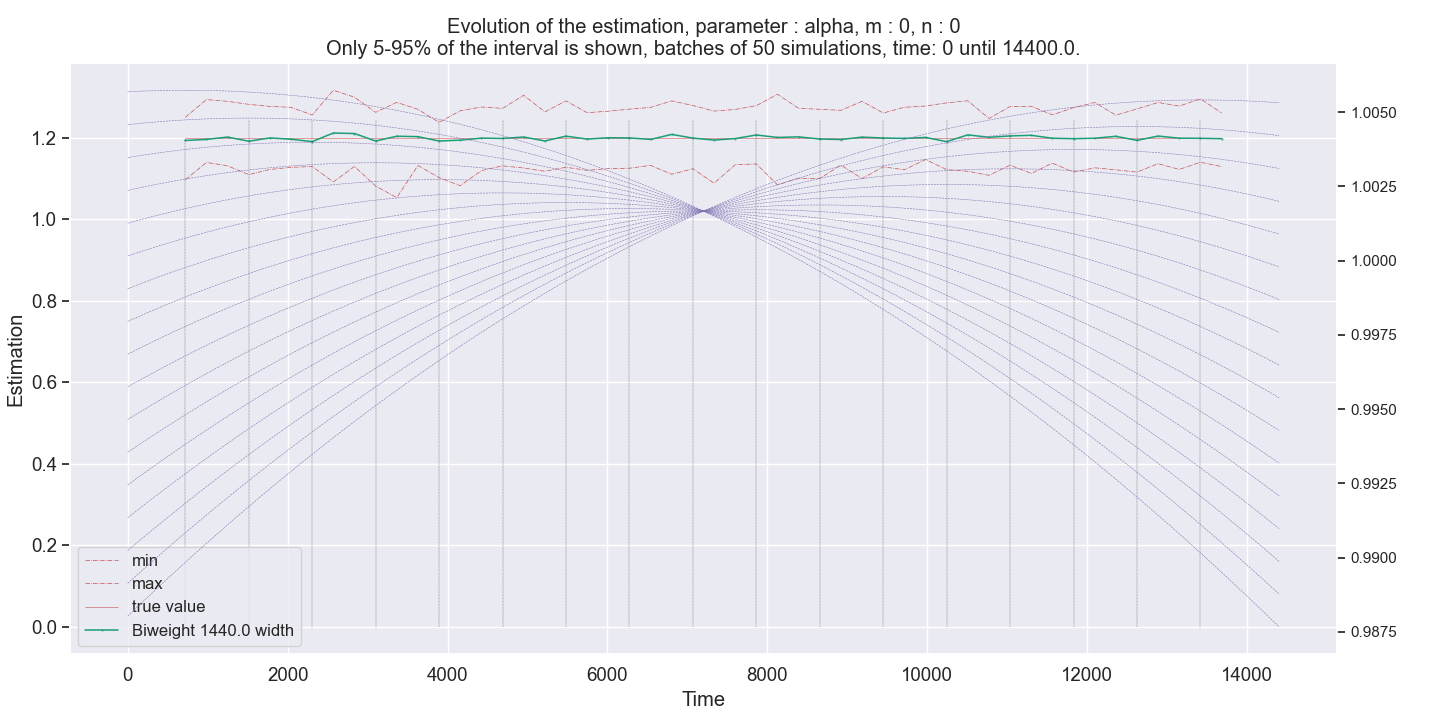
\includegraphics[width = 0.48 \textwidth]{../imag/chap3/0/Figure_10.png}
}}
\caption{TO WRITE. OBSERVATION TWO KERNELS}
\label{fig:TEST}
\end{figure}


\begin{figure}
\centering
\includegraphics[width = 0.90 \textwidth]{../imag/chap3/0/A.png}
\caption{TO WRITE.}
\label{fig:first_estimate_0_alpha}
\end{figure}

\begin{figure}
\centering
\includegraphics[width = 0.90 \textwidth]{../imag/chap3/0/B.png}
\caption{TO WRITE.}
\label{fig:first_estimate_0_beta}
\end{figure}

\begin{figure}
\centering
\includegraphics[width = 0.90 \textwidth]{../imag/chap3/0/C.png}
\caption{TO WRITE.}
\label{fig:first_estimate_0_nu}
\end{figure}











\willdo{le nom...}
\begin{figure}
\centering
\subfloat{{
\includegraphics[width = 0.48 \textwidth]{../imag/chap3/1/Figure_2.png}
}} 
\subfloat{{
\includegraphics[width = 0.48 \textwidth]{../imag/chap3/1/Figure_10.png}
}}
\caption{TO WRITE. OBSERVATION TWO KERNELS}
\label{fig:TEST}
\end{figure}

\begin{figure}
\centering
\includegraphics[width = 0.90 \textwidth]{../imag/chap3/1/D.png}
\caption{TO WRITE.}
\label{fig:first_estimate_1_alpha}
\end{figure}

\begin{figure}
\centering
\includegraphics[width = 0.90 \textwidth]{../imag/chap3/1/E.png}
\caption{TO WRITE.}
\label{fig:first_estimate_1_beta}
\end{figure}

\begin{figure}
\centering
\includegraphics[width = 0.90 \textwidth]{../imag/chap3/1/F.png}
\caption{TO WRITE.}
\label{fig:first_estimate_1_nu}
\end{figure}

















\begin{figure}
\centering
\subfloat{{
\includegraphics[width = 0.48 \textwidth]{../imag/chap3/2/Figure_2.png}
}} 
\subfloat{{
\includegraphics[width = 0.48 \textwidth]{../imag/chap3/2/Figure_10.png}
}}
\caption{TO WRITE. OBSERVATION TWO KERNELS}
\label{fig:TEST}
\end{figure}

\begin{figure}
\centering
\includegraphics[width = 0.90 \textwidth]{../imag/chap3/2/Figure_2.png}
\caption{TO WRITE.}
\label{fig:first_estimate_2_alpha}
\end{figure}

\begin{figure}
\centering
\includegraphics[width = 0.90 \textwidth]{../imag/chap3/2/Figure_3.png}
\caption{TO WRITE.}
\label{fig:first_estimate_2_beta}
\end{figure}

\begin{figure}
\centering
\includegraphics[width = 0.90 \textwidth]{../imag/chap3/2/Figure_4.png}
\caption{TO WRITE.}
\label{fig:first_estimate_2_nu}
\end{figure}



















\begin{figure}
\centering
\subfloat{{
\includegraphics[width = 0.48 \textwidth]{../imag/chap3/3/Figure_2.png}
}} 
\subfloat{{
\includegraphics[width = 0.48 \textwidth]{../imag/chap3/3/Figure_10.png}
}}
\caption{TO WRITE. OBSERVATION TWO KERNELS}
\label{fig:TEST}
\end{figure}

\begin{figure}
\centering
\includegraphics[width = 0.90 \textwidth]{../imag/chap3/3/J.png}
\caption{TO WRITE.}
\label{fig:first_estimate_3_alpha}
\end{figure}

\begin{figure}
\centering
\includegraphics[width = 0.90 \textwidth]{../imag/chap3/3/K.png}
\caption{TO WRITE.}
\label{fig:first_estimate_3_beta}
\end{figure}

\begin{figure}
\centering
\includegraphics[width = 0.90 \textwidth]{../imag/chap3/3/L.png}
\caption{TO WRITE.}
\label{fig:first_estimate_3_nu}
\end{figure}















\begin{figure}
\centering
\subfloat{{
\includegraphics[width = 0.48 \textwidth]{../imag/chap3/4/Figure_2.png}
}} 
\subfloat{{
\includegraphics[width = 0.48 \textwidth]{../imag/chap3/4/Figure_10.png}
}}
\caption{TO WRITE. OBSERVATION TWO KERNELS}
\label{fig:TEST}
\end{figure}

\begin{figure}
\centering
\includegraphics[width = 0.90 \textwidth]{../imag/chap3/4/M.png}
\caption{TO WRITE.}
\label{fig:first_estimate_4_alpha}
\end{figure}

\begin{figure}
\centering
\includegraphics[width = 0.90 \textwidth]{../imag/chap3/4/N.png}
\caption{TO WRITE.}
\label{fig:first_estimate_4_beta}
\end{figure}

\begin{figure}
\centering
\includegraphics[width = 0.90 \textwidth]{../imag/chap3/4/O.png}
\caption{TO WRITE.}
\label{fig:first_estimate_4_nu}
\end{figure}






































\newpage
\section{Second Attempt of the Adaptive Algorithm}



\begin{figure}
\centering
\includegraphics[width = 0.90 \textwidth]{../imag/chap3/4/M.png}
\caption{TO WRITE.}
\label{fig:first_estimate_4_alpha}
\end{figure}

\begin{figure}
\centering
\includegraphics[width = 0.90 \textwidth]{../imag/chap3/4/N.png}
\caption{TO WRITE.}
\label{fig:first_estimate_4_beta}
\end{figure}

\begin{figure}
\centering
\includegraphics[width = 0.90 \textwidth]{../imag/chap3/4/O.png}
\caption{TO WRITE.}
\label{fig:first_estimate_4_nu}
\end{figure}










\chapter{Package}
That work is mostly empirical as well as turned upon numerical simulations/estimations. For that reason, we built an array of tools for working on Hawkes process. We describe these here; some of them are re-usable for other project, and we include them in the personal library of the author, while the rest is specialized for Hawkes processes.

\section{CSV Files for simulations}
\label{section:files_csv}


\section{Personal Libraries}
\label{personal_lib}
With that project, I started writing my own libraries. Here is the link to my github in order to download them if anyone needs them. 

\href{https://github.com/Code-Cornelius/libraries}{https://github.com/Code-Cornelius/libraries}


\section{Architecture of my Python's Code}
\label{csv-files}
The main code is available here: 
\href{https://github.com/Code-Cornelius/Hawkes-Proccesses-with-Cohen}{https://github.com/Code-Cornelius/Hawkes-Proccesses-with-Cohen}. As a complement, let me explain some implementations choices in here.




\backmatter

\printbibliography
\nocite{*}

\addcontentsline{toc}{chapter}{References}

%\listoffigures
%\addcontentsline{toc}{chapter}{Table des figures}

\tableofcontents%table des matières plus complète
\addcontentsline{toc}{chapter}{Table of content}%ajout de la table des matières dans la table des matières !



\end{document}
